% Sumber LaTeX untuk buku ``Metode Aljabar'' dalam bahasa Mandarin
% Hak Cipta 2018  Wen-Wei Li.
% Izin diberikan untuk menyalin, mendistribusikan, dan/atau memodifikasi
% dokumen ini berdasarkan ketentuan Creative Commons
% Attribution 4.0 International (CC BY 4.0)
% http://creativecommons.org/licenses/by/4.0/

% Untuk disertakan
\chapter{Valuasi Medan}
Jika dipandang dari sudut pengetahuan yang kita miliki sekarang, valuasi merupakan objek yang alami dalam teori medan, misalnya:
\begin{itemize}
	\item Untuk suatu bilangan prima $p$, bagi setiap unsur $x \neq 0$ dari medan $\Q$ kita dapat mempertimbangkan banyaknya kemunculan $p$ dalam faktorisasi primanya, yaitu $v_p(x)$, dan menetapkan pula $v_p(0)=\infty$;
	\item Demikian pula, untuk suatu titik $x$ pada permukaan Riemann $X$ dan fungsi meromorfik $f$ pada $X$, kita dapat mempertimbangkan orde lenyap $f$ di $x$, yaitu $v_x(f) \in \Z \sqcup \{\infty\}$.
\end{itemize}
Secara lebih umum, teori valuasi mempelajari fungsi $v: A \to \Gamma \sqcup \{\infty\}$ yang memenuhi syarat-syarat tertentu, dengan $A$ suatu gelanggang komutatif dan $\Gamma$ suatu grup komutatif terurut total (misalnya grup aditif $\Z$ atau $\R$). Gagasan untuk memperbolehkan grup komutatif terurut total yang umum berasal dari Krull, sedangkan kasus yang paling lazim, $\Gamma \subset \R$, disebut valuasi peringkat $1$. Valuasi secara alami mengarah pada struktur topologis, limit, dan kelengkapan; sebagai contoh, medan bilangan $p$-adik $\Q_p$ tepat merupakan pelengkapan $\Q$ terhadap $v_p$. Pelengkapan menyediakan serangkaian alat analitis bagi kajian teori medan, seperti Lema Hensel (Teorema \ref{prop:Hensel-lemma}) yang digunakan untuk mencari akar polinomial. Konsep-konsep ini muncul secara wajar dalam teori bilangan aljabar dan geometri aljabar; buku ini hanya memberikan pengantar singkat.

Konsep yang mencakup valuasi peringkat $1$ dan sedikit lebih umum adalah nilai mutlak. Sebagai contoh, pada $\Q$ kita dapat mengambil $|\cdot|_p := p^{-v_p(\cdot)}$ (dengan $p$ prima) atau nilai mutlak biasa $|\cdot|_\infty$; teorema klasifikasi yang terkait sangat indah sekaligus cerdik.

Vektor Witt, yang diperkenalkan pada akhir bab ini, merupakan alat ampuh untuk mengangkat medan sempurna berkarakteristik $p > 0$ ke karakteristik $0$. Penerapannya mencakup, antara lain, teori kohomologi varietas aljabar berkarakteristik $p$ dalam geometri aljabar. Gagasan awalnya sangat alami: bagaimana memahami struktur aljabar $\Q_p$ dan perluasan tak-teramifikasinya melalui ekspansi $p$-adik? E.\ Witt memberikan jawaban yang elementer sekaligus cemerlang.

\begin{wenxintishi}
	Mula-mula, \S\ref{sec:filters} memuat sejumlah pengetahuan pendahuluan dan definisi tentang topologi. Bagian ini dapat dilewati apabila pembaca telah menguasai pelengkapan dengan baik, meskipun kesempatan mempelajari bahasa filter Cartan juga bermanfaat. Dalam \S\ref{sec:Krull-valuation} dan \S\ref{sec:valued-field}, kita membahas valuasi yang mengambil nilai dalam grup komutatif terurut total umum $\Gamma$, yakni valuasi Krull; namun, dalam banyak penerapan hanya kasus peringkat $1$ yang diperlukan.
	
	Tujuan \S\ref{sec:absolute-value} adalah membahas nilai mutlak beserta klasifikasinya. Selanjutnya, \S\ref{sec:closed-unit-disc} mengalihkan perhatian kepada gelanggang $K^\circ \lrangle{t}$, atau, dari sudut pandang geometris, cakram satuan tertutup. Ini merupakan model dasar bagi geometri analitik non-Archimedes sekaligus contoh menarik untuk melihat wujud teori valuasi.

	Pembahasan mengenai perluasan valuasi (\S\ref{sec:valuation-ext-1} dan \S\ref{sec:valuation-ext-2}) cukup panjang dan memerlukan sejumlah kiat, terutama dalam kasus tak lengkap, meskipun hasil akhirnya sederhana. Teori terkait kerap dijumpai dalam buku teks teori bilangan aljabar, misalnya \cite{Lai16}; kita tetap mengkajinya di sini terutama karena menganggapnya sebagai alur pemikiran yang alami. Pembaca dipersilakan menimbangnya menurut minat dan waktu yang tersedia. Pembahasan ini mengikuti pendekatan \cite[Chapter XII]{Lang02} dan \cite[Chapter II]{Neu99}.
\end{wenxintishi}

\section{Filter}\label{sec:filters}
Konsep filter dipelopori oleh H.\ Cartan; uraian terperinci dapat dilihat dalam \cite{Bou-Top1}. Filter menyediakan bahasa yang sangat ringkas untuk mengkaji konvergensi dan pelengkapan, serta memiliki banyak penerapan dalam logika matematika. Bagian ini memerlukan sejumlah pengetahuan dasar tentang topologi himpunan-titik.

\begin{definition}\index{luzi@filter (filter)}
	Sebuah \emph{filter} pada himpunan tak kosong $X$ adalah keluarga himpunan bagian $\mathfrak{F} \subset P(X)$, $\mathfrak{F} \neq \emptyset$, yang memenuhi syarat-syarat berikut:
	\begin{enumerate}[\bfseries {F}.1]
		\item Jika $A, B \in \mathfrak{F}$, maka $A \cap B \in \mathfrak{F}$ (ketertutupan ke bawah);
		\item Jika $A \in \mathfrak{F}$ dan $X \supset A' \supset A$, maka $A' \in \mathfrak{F}$ (ketertutupan ke atas);
		\item $\emptyset \notin \mathfrak{F}$.
	\end{enumerate}
	Jika keluarga himpunan bagian $\mathfrak{B} \neq \emptyset$ hanya memenuhi syarat-syarat yang lebih lemah berikut, maka $\mathfrak{B}$ disebut \emph{basis filter} pada $X$:
	\begin{enumerate}[\bfseries {FB}.1]
		\item Jika $A, B \in \mathfrak{B}$, maka terdapat $C \in \mathfrak{B}$ sedemikian sehingga $C \subset A \cap B$,
		\item $\emptyset \notin \mathfrak{B}$.
	\end{enumerate}
	Untuk suatu basis filter $\mathfrak{B}$, filter $\mathfrak{F} := \{ F \subset X: \exists B \in \mathfrak{B},\; F \supset B \}$ disebut filter yang dibangkitkan oleh $\mathfrak{B}$, dan $\mathfrak{B}$ disebut suatu basis bagi $\mathfrak{F}$. Jika $\mathfrak{F} \subset \mathfrak{F}'$ keduanya merupakan filter pada $X$, maka $\mathfrak{F}'$ disebut \emph{penghalusan} dari $\mathfrak{F}$.
\end{definition}

\begin{example}\label{eg:sequence-as-filter}
	Misalkan $(x_k)_{k=1}^\infty$ suatu barisan dalam $X$. Definisikan $\mathfrak{F}$ sebagai himpunan semua himpunan bagian $E \subset X$ yang memenuhi syarat berikut:
	\[ \exists N \geq 1, \quad k \geq N \implies x_k \in E . \]
	Syarat-syarat filter mudah diperiksa untuk $\mathfrak{F}$; semua himpunan bagian berbentuk $\{ x_k, x_{k+1}, \ldots\}$ ($k \geq N$ dapat dipilih sembarang, dengan $N \geq 1$ suatu bilangan bulat yang telah ditetapkan) membentuk suatu basis bagi $\mathfrak{F}$.
\end{example}

\begin{example}\label{eg:nbd-filter}
	Misalkan $X$ suatu ruang topologis. Untuk setiap $x \in X$, ambil $\mathfrak{N}_x$ sebagai himpunan semua lingkungan $x$: ingat bahwa $E \subset X$ merupakan lingkungan $x$ tepat ketika terdapat himpunan terbuka $U$ sedemikian sehingga $x \in U \subset E$. Jelas bahwa $\mathfrak{N}_x$ membentuk filter pada $X$. Apa yang disebut basis lingkungan $x$ dalam topologi himpunan-titik (lihat \cite[Definisi 2.6.3]{Xiong}) tidak lain adalah basis bagi filter $\mathfrak{N}_x$.

	Sesungguhnya, $\{ \mathfrak{N}_x : x \in X \}$ menentukan sepenuhnya struktur topologis $X$, sebab $V \subset X$ terbuka jika dan hanya jika $V$ merupakan lingkungan bagi setiap titiknya. Bahkan dapat dibuktikan bahwa pemberian suatu topologi pada $X$ setara dengan pemberian keluarga filter $\{ \mathfrak{N}_x  : x \in X\}$ sedemikian sehingga, untuk setiap $x$,
	\begin{compactitem}
		\item jika $E \in \mathfrak{N}_x$, maka $x \in E$;
		\item jika $E \in \mathfrak{N}_x$, maka terdapat $F \in \mathfrak{N}_x$ sedemikian sehingga $F \subset E$ dan $y \in F \implies F \in \mathfrak{N}_y$.
	\end{compactitem}
	Korespondensi tersebut dicirikan oleh $\mathfrak{N}_x = \{E : x\; \text{memiliki lingkungan }E\}$. Lihat \cite[Teorema 2.3.3]{Xiong} untuk rinciannya. Dengan demikian, struktur topologis juga dapat dirumuskan dalam bahasa filter. Kita akan segera melihat keunggulan pendekatan ini.
\end{example}

Ingat kembali grup topologis yang dibahas dalam Definisi \ref{def:topological-group}. Pada bagian ini kita hanya mempertimbangkan grup topologis komutatif Hausdorff, dengan operasi grup ditulis secara aditif. Grup-grup ini membentuk kategori $\cate{TopAb}$, yang morfismenya adalah homomorfisme grup kontinu. Dengan cara yang sama diperoleh kategori gelanggang topologis Hausdorff $\cate{TopRing}$ dan kategori medan topologis Hausdorff $\cate{TopField}$; untuk medan topologis, kita mensyaratkan bahwa inversi perkalian $K^\times \to K^\times$ juga kontinu. Lebih lanjut, kita dapat pula membicarakan modul topologis di atas gelanggang topologis. \index{tuopuhuan} \index[sym1]{TopAb@$\cate{TopAb}$, $\cate{TopRing}$, $\cate{TopField}$} \index{tuopuqun}

Selanjutnya tetapkan suatu ruang topologis $X$, dan tetap tuliskan filter lingkungan yang bersesuaian sebagai $\mathfrak{N}_x$, $x \in X$. Berdasarkan Contoh \ref{eg:sequence-as-filter}, setiap barisan $(x_k)_{k=1}^\infty$ membangkitkan filter pada $X$, sedangkan filter pada $X$ dapat dipandang sebagai suatu perumuman barisan.
\begin{description}
	\item[Konvergensi] Suatu basis filter $\mathfrak{F}$ pada $X$ dikatakan konvergen ke $x \in X$ jika setiap lingkungan $x$ memuat suatu $F \in \mathfrak{F}$, dan ditulis $\mathfrak{F} \to x$; apabila $\mathfrak{F}$ merupakan filter, ini setara dengan mengatakan bahwa $\mathfrak{F}$ adalah penghalusan dari $\mathfrak{N}_x$. Dalam keadaan ini, \textbf{FB.1} menyiratkan bahwa $x$ termasuk dalam penutupan setiap $F \in \mathfrak{F}$. Pembaca dipersilakan memeriksa bahwa semua ini sesuai dengan kasus barisan.
	\item[Pemisahan] Ruang $X$ merupakan ruang Hausdorff jika dan hanya jika setiap filter konvergen ke paling banyak satu titik.
	\item[Kontinuitas] Untuk fungsi $f: X \to Y$ dan filter $\mathfrak{F}$ pada $X$, tetapkan
		\[ f\mathfrak{F} := \left\{ F \subset Y: \exists E \in \mathfrak{F},\; F \supset f(E) \right\}, \]
		yang merupakan filter pada $Y$ (alasannya: $f(A) \cap f(B) \supset f(A \cap B)$). Faktanya, $f$ kontinu jika dan hanya jika untuk setiap $x \in X$ berlaku $(\mathfrak{F} \to x) \implies (f\mathfrak{F} \to f(x))$.
	\item[Filter Cauchy] Misalkan $(A, +)$ suatu grup topologis komutatif Hausdorff. Dalam hal ini \index{luzi!Cauchy}
		\[ \mathfrak{N}_0 + x = \mathfrak{N}_x = x + \mathfrak{N}_0, \quad -\mathfrak{N}_0 = \mathfrak{N}_0. \]
		Suatu filter $\mathfrak{F}$ pada $A$ disebut \emph{filter Cauchy} jika untuk setiap lingkungan $U \in \mathfrak{N}_0$ terdapat $E \in \mathfrak{F}$ sedemikian sehingga
		\[ E-E := \left\{x-y: x,y \in E \right\} \subset U. \]
		Basis filter Cauchy didefinisikan dengan sifat yang sama; basis-basis tersebut membangkitkan filter Cauchy.
		\begin{compactenum}[(a)]
			\item Langsung dari definisi terlihat bahwa setiap penghalusan filter Cauchy tetap merupakan filter Cauchy.
			\item Untuk setiap $x \in A$, keluarga lingkungan $\mathfrak{N}_x$ merupakan filter Cauchy: memang, dari kontinuitas operasi grup, untuk $U$ yang diberikan dapat dipilih $E_0 \in \mathfrak{N}_0$ sedemikian sehingga $E_0 - E_0 \subset U$; dengan demikian $E := x + E_0 \in \mathfrak{N}_x$ memenuhi $E-E = E_0 - E_0 \subset U$.
			\item Jadi, setiap filter konvergen $\mathfrak{F}$ pasti merupakan filter Cauchy, sebab dalam hal ini $\mathfrak{F}$ adalah penghalusan dari suatu $\mathfrak{N}_x$.
		\end{compactenum}
		Selain itu, homomorfisme kontinu antarkelompok topologis $f: A \to B$ memetakan setiap filter Cauchy $\mathfrak{F}$ ke filter Cauchy $f\mathfrak{F}$: untuk suatu lingkungan $V$ dari $0 \in B$, kontinuitas $f$ memungkinkan kita memilih lingkungan $U$ dari $0 \in A$ sedemikian sehingga $f(U) \subset V$; kemudian pilih $E \in \mathfrak{F}$ sehingga $E-E \subset U$. Maka $F := f(E) \in f\mathfrak{F}$ memenuhi
		\[ F - F = f(E-E) \subset f(U) \subset V. \]
		Dengan cara yang sama, pembaca dipersilakan memeriksa bahwa semua ini sesuai dengan konsep klasik barisan Cauchy.
	\item[Kelengkapan] Jika setiap filter Cauchy dalam grup topologis komutatif $A$ konvergen, maka $A$ disebut \emph{lengkap}. Kelengkapan pada umumnya hanya dibahas untuk ruang Hausdorff.
\end{description}

Jika untuk setiap $x \in X$ filter $\mathfrak{N}_x$ mempunyai basis terhitung, maka $X$ dikatakan memenuhi aksioma keterhitungan pertama. Contohnya mencakup ruang metrik biasa $(X, d)$, sebab semua bola terbuka berpusat di $x$ dengan jari-jari-$d$ sebesar $\frac{1}{2}, \frac{1}{3}, \ldots$ memberikan suatu basis terhitung. Di bawah aksioma keterhitungan pertama, barisan dapat menggantikan filter dalam pencirian sifat-sifat topologis di atas; ini merupakan pengetahuan standar dalam topologi himpunan-titik, lihat \cite[\S 5.1]{Xiong}.

Untuk grup topologis komutatif Hausdorff $A$, suatu \emph{pelengkapan} adalah morfisme $\iota: A \to \hat{A}$ dalam kategori $\cate{TopAb}$ yang memenuhi \index{wanbeihua}
\begin{compactenum}[(\bfseries {CO}.1)]
	\item $\iota: A \to \iota(A)$ merupakan homeomorfisme,
	\item $\iota(A) \subset \hat{A}$ rapat,
	\item $\hat{A}$ lengkap dalam pengertian filter Cauchy.
\end{compactenum}
Proposisi \ref{prop:completion-ring-characterization} akan membuktikan bahwa sifat-sifat ini mencirikan $(\hat{A}, \iota)$ secara tunggal. Konstruksi keberadaannya telah diuraikan dalam \S\ref{sec:group-limit}; di bawah ini kita akan menanganinya menggunakan filter, pada dasarnya mengikuti pendekatan \cite[\S 8]{Str06}. Pembaca juga dapat merujuk ke \cite[Chapitre III]{Bou-Top1}. Karena keterbatasan ruang dan cakupan pembahasan, verifikasi yang panjang akan dihilangkan.

\begin{asparaenum}
	\item Pertama, untuk setiap basis filter $\mathfrak{B}$ pada $A$, definisikan
	\begin{gather}\label{eqn:min-Cauchy-filter}
		\hat{\mathfrak{B}} := \text{filter yang dibangkitkan oleh basis filter}\; \left\{ B+U: B \in \mathfrak{B},\; U \ni 0: \text{lingkungan terbuka} \right\} \;\text{.}
	\end{gather}
	Jika $\mathfrak{B}$ merupakan basis bagi filter Cauchy $\mathfrak{F}$, maka $\hat{\mathfrak{B}}$ memberikan filter Cauchy terkecil yang termuat dalam $\mathfrak{F}$; filter yang diperoleh dengan cara ini dapat disebut \emph{filter Cauchy minimal}.

	\item Mengambil kasus khusus $\mathfrak{B} = \{\{x\}\}$ menghasilkan $\hat{\mathfrak{B}} = \mathfrak{N}_x$, sehingga semua $\mathfrak{N}_x$ merupakan filter Cauchy minimal. Sekarang definisikan
	\begin{align*}
		\iota: A & \longrightarrow \hat{A} := \left\{ \mathfrak{F}: A\; \text{memiliki filter Cauchy minimal }\mathfrak{F} \right\} \\
		x & \longmapsto \hat{x} = \mathfrak{N}_x.
	\end{align*}
	Untuk filter Cauchy minimal $\mathfrak{F}, \mathfrak{G}$, kita dapat membentuk basis filter Cauchy $\{ F+G : F \in \mathfrak{F}, G \in \mathfrak{G} \}$ dan $\{ -F: F \in \mathfrak{F} \}$; kemudian ambil filter Cauchy minimal yang bersesuaian melalui \eqref{eqn:min-Cauchy-filter}. Dengan demikian diperoleh struktur grup komutatif pada $\hat{A}$. Struktur ini menjadikan $\iota$ suatu homomorfisme grup. Karena $A$ merupakan ruang Hausdorff, $\iota$ injektif. Mudah diperiksa bahwa $\hat{0} := \mathfrak{N}_0$ merupakan unsur identitas dari $(\hat{A}, +)$.

	\item Berikan topologi berikut pada $\hat{A}$. Untuk filter $\hat{x} \in \hat{A}$ dan setiap $U \in \hat{x}$, definisikan
	\begin{gather}\label{eqn:filter-dagger}
		U^\dagger := \left\{ \mathfrak{F} \in \hat{A} : U \in \mathfrak{F} \right\}, \quad \mathfrak{N}_{\hat{x}} := \{ U^\dagger: U \in \hat{x} \};
	\end{gather}
	Ketertutupan ke atas menunjukkan bahwa $U \subset V \implies U^\dagger \subset V^\dagger$. Ini menentukan struktur grup topologis pada $\hat{A}$ sedemikian sehingga $\mathfrak{N}_{\hat{x}}$ memberikan basis lingkungan bagi $\hat{x}$. Selain itu, karena filter Cauchy dalam $\hat{A}$ bersifat minimal, kita mempunyai $\bigcap_{U \in \mathfrak{N}_0} U^\dagger = \left\{ \mathfrak{F} \in \hat{A}: \mathfrak{F} \supset \mathfrak{N}_0 \right\} = \{\hat{0}\}$; maka \eqref{eqn:top-group-Hausdorff} segera menunjukkan bahwa $\hat{A}$ merupakan ruang Hausdorff.
	
	\item Kita harus memeriksa bahwa $\iota$ memberikan homeomorfisme $A \rightiso \iota(A)$. Pertimbangkan suatu lingkungan terbuka $U \in \hat{x} = \mathfrak{N}_x$ dari $x \in X$; jelas bahwa $\iota^{-1}(U^\dagger) = \{y: U \in \mathfrak{N}_y \} = U$, sehingga $\iota$ merupakan homeomorfisme. Selanjutnya, kerapatan $\iota(A)$ dibuktikan sebagai berikut. Tetapkan basis filter Cauchy $\mathfrak{B}$, bentuk $\hat{\mathfrak{B}}$, dan pertimbangkan lingkungannya $U^\dagger$ ($U \in \hat{\mathfrak{B}}$); kita harus membuktikan $U^\dagger \cap \iota(A) \neq \emptyset$. Kita boleh mengandaikan $U = B+V$, dengan $B \in \mathfrak{B}$ dan $V \ni 0$ suatu lingkungan dalam $A$. Untuk setiap $b \in B$, dari $b+V \subset U$ diperoleh $U \in \mathfrak{N}_b$, yakni $\iota(b) \in U^\dagger$.

	\item Terakhir, mengenai kelengkapan: misalkan $\hat{\mathfrak{F}}$ suatu filter Cauchy pada $\hat{A}$, dan tetapkan
	\[ \mathfrak{G}_0 := \left\{ U \subset A : U \neq \emptyset, \; U^\dagger \in \hat{\mathfrak{F}} \right\}, \qquad \text{lihat \eqref{eqn:filter-dagger}. } \]
	Dapat dibuktikan bahwa $\mathfrak{G}_0$ merupakan basis filter Cauchy pada $A$, dan bahwa $\hat{\mathfrak{F}}$ konvergen ke filter Cauchy minimal yang bersesuaian, $\mathfrak{G} \in \hat{A}$.
\end{asparaenum}

Selanjutnya andaikan $A$ suatu gelanggang topologis, dan tuliskan pemetaan perkaliannya sebagai $m$. Dalam keadaan ini, struktur gelanggang topologis dapat diperluas ke $\hat{A}$, dan $A$ komutatif jika dan hanya jika $\hat{A}$ komutatif. Pokoknya ialah membuktikan bahwa jika $\mathfrak{F}, \mathfrak{G}$ merupakan basis filter Cauchy pada $A$, maka citranya $m(\mathfrak{F}, \mathfrak{G})$ juga demikian. Perhatikan persamaan
\begin{gather*}
	x'y' - xy = (x'-x)y_1 + x_1 (y'-y) + (x' - x)(y' - y_1) + (x - x_1)(y'-y).
\end{gather*}
Untuk lingkungan $0 \in W \subset A$ yang cukup kecil, selama $x,x'$ (atau $y,y'$) diambil dari suatu himpunan bagian $F$ (atau $G$) yang cukup kecil dalam $\mathfrak{F}$ (atau $\mathfrak{G}$), dapat dipastikan bahwa $(x'-x)(y'-y) \in W$. Pilih pula $(x_1, y_1) \in F \times G$; maka $(x' - x)(y' - y_1) + (x - x_1)(y'-y) \in W + W$. Sekarang tetapkan $(x_1, y_1)$. Dengan menggunakan kontinuitas perkalian, kita dapat memilih $F \supset F^\dagger \in \mathfrak{F}$ dan $G \supset G^\dagger \in \mathfrak{G}$ sedemikian sehingga, apabila $x,x' \in F^\dagger$ dan $y,y' \in G^\dagger$, berlaku $(x'-x)y_1 \in W$ dan $x_1(y'-y) \in W$. Jadi, $x'y' - xy \in 4 W$, yang menunjukkan bahwa $m(\mathfrak{F}, \mathfrak{G})$ merupakan basis filter Cauchy.

\begin{proposition}\label{prop:completion-ring-characterization}
	Pelengkapan $\iota: A \to \hat{A}$ mempunyai sifat universal berikut: untuk setiap grup topologis komutatif Hausdorff lengkap $B$ dan morfisme $f: A \to B$ dalam $\cate{TopAb}$, terdapat tepat satu morfisme $\hat{f}: \hat{A} \to B$ yang membuat diagram berikut komutatif:
	\[\begin{tikzcd}
	A \arrow[r, "\iota"] \arrow[rd, "f"'] & \hat{A} \arrow[d, "\exists! \;\hat{f}"] \\
	& B
	\end{tikzcd}\]
	Apabila $A$ diberikan, data $(\hat{A}, \iota)$ dengan demikian tunggal hingga isomorfisme tunggal, dan disebut \emph{pelengkapan} $A$. Pernyataan ini tetap berlaku untuk kategori $\cate{TopRing}$.
\end{proposition}
\begin{proof}
	Di bawah ini kita hanya menggunakan sifat \textbf{CO.1} --- \textbf{CO.3}, tanpa bergantung pada konstruksi khusus $(\hat{A}, \iota)$. Ketunggalan $(\hat{A}, \iota)$ merupakan prinsip umum teori kategori; lihat \S\ref{sec:cat-universals}. Untuk suatu $\hat{x} \in \hat{A}$, syarat-syarat pada $\iota$ menjamin bahwa $\{\iota^{-1}(U): U \in \mathfrak{N}_{\hat{x}} \}$ membangkitkan filter Cauchy $\mathfrak{N}^\flat_{\hat{x}}$ pada $A$. Karena $B$ lengkap dan Hausdorff serta $f$ kontinu, $f\mathfrak{N}^\flat_{\hat{x}}$ mempunyai limit tunggal $\hat{f}(\hat{x})$; juga mudah dilihat bahwa $\hat{f}\iota = f$. Dari konstruksi ini kita sekaligus memperoleh bahwa $\hat{f}(\hat{x})$ termasuk dalam penutupan $f(\iota^{-1}(U))$ di $B$ untuk setiap $U \in \mathfrak{N}_{\hat{x}}$.

	Selanjutnya kita tunjukkan bahwa $\hat{f}$ yang didefinisikan di atas kontinu; ketunggalan $\hat{f}$ merupakan akibat langsung dari kerapatan. Misalkan $V$ suatu lingkungan dari $y := \hat{f}(\hat{x})$. Paragraf sebelumnya menunjukkan bahwa terdapat $U \in \mathfrak{N}_{\hat{x}}$ yang terbuka sedemikian sehingga $f(\iota^{-1}(U)) \subset V$; kita ingin membuktikan $\hat{f}(U) \subset V$. Karena $U$ merupakan lingkungan bagi setiap unsurnya, paragraf sebelumnya memberikan bahwa $\hat{f}(U)$ termuat dalam penutupan $f(\iota^{-1}(U))$, sehingga termuat dalam penutupan $V$.	Akan tetapi, Lema \ref{prop:top-group-separation} menyatakan bahwa $y$ mempunyai basis lingkungan tertutup, dan ini membuktikan klaim tersebut.
\end{proof}
Secara khusus, jika $f: A \to B$ merupakan morfisme dalam $\cate{TopAb}$ atau $\cate{TopRing}$, dengan menerapkan sifat universal pada morfisme komposit $A \xrightarrow{f} B \to \hat{B}$ segera diperoleh tepat satu $\hat{f}$ yang membuat diagram
$\begin{tikzcd}[row sep=small, column sep=small]
	A \arrow[r, "f"] \arrow[d] & B \arrow[d] \\
	\hat{A} \arrow[r, "\hat{f}"'] & \hat{B}
\end{tikzcd}$
komutatif. Ini disebut kefunktoran pelengkapan: sebagai contoh, dalam kasus grup komutatif, $A \mapsto \hat{A}$ menentukan suatu funktor dari $\cate{TopAb}$ ke subkategori penuh $\cate{ComTopAb}$ yang terdiri atas grup-grup lengkap.

Secara umum, pelengkapan $\hat{K}$ dari medan topologis $K$ sebagai gelanggang belum tentu merupakan medan; lihat \cite[Example 8.59]{Str06} untuk suatu contoh tandingan. Syarat perlu yang jelas agar $\hat{K}$ menjadi medan topologis ialah
\begin{equation}\label{eqn:field-completion}
	\begin{tikzcd}[row sep=tiny, column sep=small]
		K^\times \arrow[r, "\sim"] & K^\times \\
		x \arrow[mapsto, r] \arrow[sloped, phantom, u, "\in" description] & x^{-1} \arrow[sloped, phantom, u, "\in" description]
	\end{tikzcd}
	 \quad\text{diperluas secara kontinu menjadi}\quad \hat{K} \smallsetminus \{0\} \to \hat{K} \smallsetminus \{0\}.
\end{equation}
Syarat ini juga cukup, sebab persamaan $x^{-1}x=1=xx^{-1}$ meluas ke $\hat{K}$ berkat kontinuitas; lihat pula \cite[III.6, Proposition 7]{Bou-Top1}. Apabila struktur topologis berasal dari valuasi atau nilai mutlak, \eqref{eqn:field-completion} selalu terpenuhi; inilah pokok bahasan \S\ref{sec:valued-field} dan \S\ref{sec:absolute-value}.

\section{Valuasi Krull dan Pelengkapan}\label{sec:Krull-valuation}
Semua gelanggang yang dibahas pada bagian ini adalah gelanggang komutatif tak nol. Kita mulai dengan meninjau garis besar valuasi melalui dua kasus dalam Contoh \ref{eg:field-basic-examples}.

\begin{example}[Bilangan $p$-adik]\label{eg:p-adic-valuation} \index{bilangan $p$-adik ($p$-adic numbers)}\index[sym1]{$v_p$}\index[sym1]{Z_p}
	Topologi biasa pada medan $\Q$ berasal dari metrik yang diberikan oleh fungsi nilai mutlak, yang dalam teori bilangan sering ditulis $|\cdot|_\infty$: dua bilangan rasional $x,y$ berdekatan berarti $|x-y|_\infty \ll 1$. Secara umum, nilai mutlak pada $\Q$ adalah fungsi bernilai riil yang memenuhi
	\begin{inparaenum}[(a)]
		\item $|x| \geq 0$ dan $|x|=0 \iff x=0$,
		\item $|xy|=|x| |y|$,
		\item ketaksamaan segitiga $|x+y| \leq |x|+|y|$
	\end{inparaenum}
	Dari suatu nilai mutlak diturunkan metrik $d(x,y)=|y-x|$ pada $\Q$, sehingga $\Q$ memperoleh topologi. Sekarang, untuk suatu bilangan prima $p$, kita ingin mendefinisikan nilai mutlak lain $x \mapsto |x|_p \in \R_{\geq 0}$ pada $\Q$ sedemikian sehingga
	\[ x \;\text{``dekat dengan''}\; y \iff |x-y|_p \ll 1 \iff x-y \in  p^n \cdot \frac{r}{s}, \quad n \gg 0, \; (p,s)=1. \]
	Untuk itu, definisikan valuasi $p$-adik setiap $a \in \Z$ sebagai
	\[ v_p(a) := \sup \left\{n \in \Z: a \in p^n \Z  \right\},\quad v_p(0) = \infty. \]
	Tidak ada masalah jika kita menetapkan $x + \infty = \infty$; dengan demikian $v_p(ab) = v_p(a) + v_p(b)$, dan persamaan ini memperluas $v_p$ secara alami ke $\Q \to \Z \sqcup \{\infty\}$. Ini memberikan nilai mutlak $p$-adik
	\[ |x|_p := p^{-v_p(x)}, \quad |0|_p = p^{-\infty} := 0. \]
	Tidak sulit memeriksa bahwa $v_p(x+y) \geq \min\{v_p(x), v_p(y)\}$, atau secara bersesuaian $|x+y|_p \leq \max\{|x|_p , |y|_p\} \leq |x|_p + |y|_p$; ini disebut ketaksamaan segitiga kuat. Jadi, $|\cdot|_p$ memang merupakan nilai mutlak pada $\Q$, atau dengan kata lain memberikan suatu ukuran ``jarak''. Secara khusus, konsep barisan Cauchy dalam analisis tetap berlaku bagi $|\cdot|_p$; dengan meniru cara membangun $\R$ dari $\Q$, kita dapat mengambil pelengkapan
	\begin{gather*}
		\Z \leadsto \Z_p, \quad	\Q \leadsto \Q_p.
	\end{gather*}
	Keduanya masing-masing tetap memiliki struktur gelanggang dan medan, dan $v_p$ (atau $|\cdot|_p$) juga tetap terdefinisi. Sebagai contoh, $\lim_{k \to \infty} p^k = 0$, sedangkan barisan $1 + p + \cdots + p^n = \frac{1 - p^{n+1}}{1 - p}$ konvergen ke $(1-p)^{-1}$ dalam $\Z_p$.

	Dengan menelaah konstruksi di atas secara saksama (lihat Proposisi \ref{prop:invert-pi}), kita mendapati bahwa $\Z_p$ tepat merupakan gelanggang bilangan bulat $p$-adik yang dibangun dalam bahasa teori gelanggang pada Contoh \ref{eg:Z_p}, sedangkan $\Q_p$ sama dengan medan pecahan $\Z_p$; sesungguhnya $\Z_p = \{x \in \Q_p: v_p(x) \geq 0 \}$. Gagasan ini pertama kali dikemukakan oleh K.\ Hensel pada tahun 1897. Untuk perluasan hingga dari $\Q$, penggantian bilangan prima dengan ideal prima menghasilkan pernyataan serupa. Istilah bilangan $p$-adik akan memperoleh penjelasan yang wajar dalam \S\ref{sec:Witt-vector}.
\end{example}

\begin{example}\label{eg:function-field-valuation} \index[sym1]{$v_x$}\index{hanshuyu}
	Sekarang pertimbangkan medan fungsi rasional satu variabel $\CC(t)$. Perkenalkan ruang projektif kompleks berdimensi satu $\mathbb{P}^1 := \CC \sqcup \{\text{titik di tak hingga}\}$, atau bola Riemann, yang merupakan arena dasar teori fungsi kompleks. Untuk setiap $x \in \mathbb{P}^1$, definisikan valuasi $f \mapsto v_x(f)$ sebagai orde lenyap $f \in \CC(t)$ di $x$, yaitu
	\[ f(t) = a_k (t - x)^k + \text{suku berderajat lebih tinggi}, \quad k = v_x(f), \; a_k \in \CC \smallsetminus \{0\}. \]
	Jika $x$ adalah titik di tak hingga, definisikan $v_x(f/g) = \deg g - \deg f$ (renungkanlah). Dengan demikian, $v_x: \CC(t) \to \Z \sqcup \{\infty\}$ juga memiliki sifat-sifat yang serupa dengan valuasi $p$-adik di atas. Ambil saja $x=0$; pelengkapan terhadap nilai mutlak $|\cdot|_x := e^{-v_x(\cdot)}$ menghasilkan
	\[ \CC(t) \leadsto \text{gelanggang deret Laurent}\;\CC(\!(t)\!), \quad \CC[t] \leadsto \text{gelanggang deret pangkat formal}\;\CC\llbracket t \rrbracket. \]
	Secara lebih umum, pertimbangkan medan fungsi meromorfik $\CC(X)$ dari sebarang permukaan Riemann kompak $X$, beserta orde lenyapnya di $x \in X$ (yang didefinisikan dalam koordinat lokal); teori serupa tetap berlaku.
\end{example}

Sekarang kita definisikan valuasi secara umum. Pertama-tama, ``nilai'' yang diberikan harus terletak dalam suatu grup komutatif terurut total $\Gamma$. Dalam bab ini, operasi biner pada $\Gamma$ biasanya ditulis secara aditif; contoh standarnya adalah $\R$ beserta subgrup-subgrup aditifnya.
\begin{definition}\index{quanxujiaohuanqun@grup komutatif terurut total (totally ordered abelian group)}
	Grup komutatif terurut total adalah suatu grup komutatif $(\Gamma, +)$ yang dilengkapi dengan himpunan bagian $P \subset \Gamma$ dan memenuhi
	\begin{compactitem}
		\item $\Gamma = P \sqcup \{0\} \sqcup (-P)$,
		\item $P + P \subset P$.
	\end{compactitem}
	Data ini menentukan urutan total pada $\Gamma$: $x < y \iff y-x \in P$, dan $P = \{x \in \Gamma: x > 0 \}$. Jadi, memberikan $(\Gamma, P)$ setara dengan memberikan $(\Gamma, \leq)$.
\end{definition}
Semua grup komutatif terurut total membentuk suatu kategori terhadap homomorfisme yang mempertahankan urutan. Dengan demikian kita dapat membicarakan isomorfisme, penyisipan, dan sebagainya untuk grup komutatif terurut total. Sifat-sifat berikut berlaku bagi setiap grup komutatif terurut total $\Gamma$:
\begin{compactitem}
	\item $x \leq x'$, $y \leq y'$ menyiratkan $x+y \leq x'+y'$;
	\item $x \leq 0 \iff (-x) \geq 0$;
	\item $\Gamma$ bebas torsi: $(n \in \Z_{\geq 1}) \wedge (nx=0) \implies x=0$, sebab $x > 0$ (atau $x < 0$) akan mengakibatkan $nx > 0$ (atau $nx < 0$).
\end{compactitem}

Demi kemudahan penulisan, kita lazim memperluas $\Gamma$ menjadi himpunan terurut total $\Gamma \sqcup \{\infty\}$ sedemikian sehingga $\forall x \in \Gamma,\; x < \infty$, dan memperluas penjumlahan pada $\Gamma$ dengan menetapkan $\forall x,\; x + \infty = \infty$.

\begin{definition}[W.\ Krull]\label{def:Krull-valuation}\index{fuzhi@valuasi (valuation)}
	Misalkan $A$ suatu gelanggang dan $(\Gamma, \leq)$ suatu grup komutatif terurut total. Suatu \emph{valuasi} pada gelanggang $A$ dengan \emph{grup nilai} $\Gamma$ adalah pemetaan $v: A \to \Gamma \sqcup \{\infty\}$ yang memenuhi sifat-sifat berikut:
	\begin{gather}
		v(xy) = v(x) + v(y), \quad x,y \in A, \label{eqn:valuation-homo} \\
		v(x+y) \geq \min\left\{ v(x), v(y) \right\}, \label{eqn:valuation-ineq} \\
		v(1) = 0, \quad v(0)=\infty \label{eqn:valuation-calibration}.
	\end{gather}
	Selain itu, kita mensyaratkan bahwa $v(A) \smallsetminus \{\infty\}$ membangkitkan grup $\Gamma$. Jika terdapat penyisipan grup komutatif terurut total $\Gamma \hookrightarrow \R$, maka $v$ disebut \emph{valuasi peringkat $1$}.
\end{definition}
Istilah peringkat $1$ berkaitan dengan peringkat grup nilai; hal ini akan dijelaskan dalam latihan.

Periksalah bahwa $v_p: \Q \to \Z \sqcup \{\infty\}$ dalam Contoh \ref{eg:p-adic-valuation} memang memenuhi syarat-syarat valuasi. Dalam kasus valuasi peringkat $1$, kita dapat memilih $q \in \R_{>1}$ dan mendefinisikan $|\cdot| := q^{-v(\cdot)}$, sehingga definisi valuasi diterjemahkan menjadi $|xy|=|x| |y|$, $|1|=1$, $|0|=0$, dan ketaksamaan segitiga kuat $|x+y| \leq \max\{|x|, |y|\}$. Sudut pandang ini akan dibahas secara terperinci dalam \S\ref{sec:absolute-value}; lihat Proposisi \ref{prop:abs-equivalence}.

Tentu saja, hasil serupa diperoleh jika operasi grup pada $\Gamma$ ditulis secara multiplikatif, urutannya dibalik, dan simbol $0$ dipakai menggantikan $\infty$; banyak pustaka menggunakan perumusan ini. Namun, perubahan tersebut hanya menyangkut notasi; yang penting adalah struktur grup nilainya.

\begin{lemma}\label{prop:valuation-generalities}
	Misalkan $v: A \to \Gamma \sqcup \{\infty\}$ suatu valuasi.
	\begin{enumerate}[(i)]
		\item Jika $x \in A^\times$, maka $v(x^{-1}) = -v(x) \in \Gamma$;
		\item Valuasi akar satuan selalu nol: jika $y^n = 1$ ($n \geq 1$), maka $v(y)=0$; khususnya, $v(-1)=0$;
		\item $v^{-1}(\infty) = \{x \in A: v(x) = \infty \} \subsetneq A$ merupakan ideal prima;
	\end{enumerate}
\end{lemma}
\begin{proof}
	Untuk (i), terapkan $v(x^{-1})+v(x) = v(1)=0$. Untuk (ii), gunakan bahwa $\Gamma$ bebas torsi. Sifat $x+\infty=\infty$, \eqref{eqn:valuation-homo}, dan \eqref{eqn:valuation-ineq} bersama-sama menghasilkan (iii).
\end{proof}
Dengan demikian, $v$ berfaktor melalui $A/v^{-1}(\infty) \xrightarrow{v} \Gamma \sqcup \{\infty\}$; karena itu, ketika mengkaji sifat-sifat umum valuasi, kita sering mengandaikan $v^{-1}(\infty) = \{0\}$.

Ketaksamaan \eqref{eqn:valuation-ineq} sesungguhnya menyiratkan sifat yang lebih kuat.
\begin{lemma}\label{prop:ultrametric}
	Misalkan $v: A \to \Gamma \sqcup \{\infty\}$ suatu valuasi. Untuk setiap $n \geq 1$ berlaku
	\[ v(x_1 + \cdots + x_n) \geq \min\left\{ v(x_1), \ldots, v(x_n)  \right\}, \quad x_1, \ldots, x_n \in A. \]
	Jika terdapat $i$ sedemikian sehingga $j \neq i \implies v(x_j) > v(x_i)$, maka $v(x_1 + \cdots + x_n) = v(x_i)$.
\end{lemma}
\begin{proof}
	Pernyataan pertama mudah diperoleh secara rekursif dari kasus $n=2$. Sekarang andaikan $\left\{v(x_j)\right\}_{j=1}^n$ mencapai nilai minimum hanya pada indeks $i$, dengan $n \geq 2$. Tetapkan $x := x_i$ dan $y := \sum_{j \neq i} x_j$. Maka $v(y) \geq \min\{ v(x_j) : j \neq i \} > v(x)$. Jika $v(x_1 + \cdots + x_n) = v(x+y) > v(x)$, maka dari
	\[ v(x) = v(x+y-y) \geq \min\{v(x+y), v(-y) \} = \min\{ v(x+y), v(y) \} > v(x) \]
	diperoleh suatu kontradiksi.
\end{proof}

Valuasi $v$ menginduksi struktur topologis pada $A$. Dengan membandingkannya dengan contoh pada awal bagian ini, pendekatan yang wajar dimulai dari
\[ U_\epsilon := \{x \in A: v(x) > \epsilon \}, \quad \epsilon \in \Gamma \]
Sifat-sifat dasar $v$ segera memberikan $U_\epsilon + U_\eta \subset U_{\min\{\epsilon, \eta\}}$, $U_\epsilon U_\eta \subset U_{\epsilon+\eta}$, dan $-U_\epsilon = U_\epsilon$. Jadi, $A$ mempunyai struktur topologis sedemikian sehingga
\begin{compactitem}
	\item suatu basis lingkungan di $0$ diberikan oleh semua $U_\epsilon$;
	\item operasi gelanggang $(x,y) \mapsto x+y$, $(x,y) \mapsto xy$, dan $x \mapsto -x$ semuanya merupakan pemetaan kontinu;
	\item $\bigcap_\epsilon U_\epsilon = v^{-1}(\infty)$.
\end{compactitem}
Butir kedua menunjukkan bahwa $A$ memang merupakan gelanggang topologis. Butir ketiga bersama \eqref{eqn:top-group-Hausdorff} menunjukkan bahwa $A$ merupakan ruang Hausdorff jika dan hanya jika $v^{-1}(\infty) = \{0\}$. Selanjutnya kita selalu mengandaikan $v^{-1}(\infty) = \{0\}$.

\begin{lemma}\label{prop:valuation-openness}
	Untuk setiap $\gamma \in \Gamma$, himpunan bagian $\{x \in A: v(x) = \gamma\}$ terbuka; sedangkan $\{x \in A : v(x) \geq \gamma\}$ dan $\{x \in A: v(x) > \gamma\}$ keduanya terbuka sekaligus tertutup.
\end{lemma}
\begin{proof}
	Lema \ref{prop:ultrametric} memberikan $\{x: v(x) = \gamma\} = \bigcup_{x: v(x) = \gamma} (x + U_\gamma)$, sehingga himpunan ini terbuka. Dengan cara yang sama, $\{x: v(x) \geq \gamma\}$ terbuka. Pernyataan kedua langsung diperoleh dari $\{ x : v(x) \geq \gamma \} = A \smallsetminus \bigcup_{\eta < \gamma} \{ x : v(x) = \eta \}$ dan $\{ x : v(x) > \gamma \} = A \smallsetminus \bigcup_{\eta \leq \gamma} \{ x : v(x) = \eta \}$.
\end{proof}

Selanjutnya kita telaah topologi pada $A$ beserta pelengkapannya. Jika $\Gamma \subset \R$ (valuasi peringkat $1$), maka $|\cdot| := e^{-v(\cdot)}$ memberi $A$ struktur ruang metrik $d(x,y) = |x-y|$. Secara khusus, $A$ memenuhi aksioma keterhitungan pertama dalam topologi, sifat-sifat topologisnya dapat dinyatakan melalui konvergensi barisan, dan teori pelengkapan yang lazim dapat diterapkan secara langsung.

Di bawah ini kita menggunakan teori filter yang diperkenalkan dalam \S\ref{sec:filters} untuk beralih ke kasus umum. Pertama, Proposisi \ref{prop:completion-ring-characterization} digunakan untuk membentuk pelengkapan $\iota: A \hookrightarrow \hat{A}$ dalam kategori $\cate{TopRing}$. Langkah kedua adalah memperluas $v: A \to \Gamma \sqcup \{\infty\}$ menjadi valuasi $\hat{v}: \hat{A} \to \Gamma \sqcup \{\infty\}$; untuk itu diperlukan lema berikut.

\begin{lemma}\label{prop:valuation-of-Cauchy-filter}
	Misalkan $\mathfrak{F}$ suatu filter Cauchy pada $A$. Tepat satu dari dua keadaan berikut pasti terjadi:
	\begin{compactenum}[(i)]
		\item Terdapat $F \in \mathfrak{F}$ dan $\gamma \in \Gamma$ sedemikian sehingga $x \in F \implies v(x) = \gamma$;
		\item Untuk setiap $\gamma \in \Gamma$, selalu terdapat $F \in \mathfrak{F}$ sedemikian sehingga $F \subset U_\gamma$.
	\end{compactenum}
	Nilai $\gamma$ dalam keadaan (i) bersifat tunggal. Keadaan (ii) terjadi jika dan hanya jika $\mathfrak{F} \to 0$.
\end{lemma}
\begin{proof}
	Pertama andaikan bahwa untuk setiap $(\gamma, F) \in \Gamma \times \mathfrak{F}$ terdapat $x \in F$ yang memenuhi $v(x) > \gamma$. Menurut definisi filter Cauchy, tetapkan dahulu $\gamma$, kemudian pilih $F$ cukup kecil agar $F-F \subset U_\gamma$. Berdasarkan Lema \ref{prop:ultrametric}, untuk setiap $y \in F$ berlaku $v(y) \geq \min\{v(x), v(y-x) \} > \gamma$; inilah keadaan (ii). Jelas bahwa (ii) setara dengan $\mathfrak{F} \to 0$.

	Jika pengandaian sebelumnya tidak berlaku, terdapat $(\eta, F)$ sedemikian sehingga $x \in F \implies v(x) \leq \eta$. Kita dapat kembali memperkecil $F$ agar $F-F \subset U_\eta$. Maka, untuk setiap $x,y \in F$, berlaku $v(x) = \min\{v(y), v(x-y) \} = v(y)$. Tuliskan nilai ini sebagai $\gamma$; inilah keadaan (i). Karena definisi menjamin bahwa irisan setiap $F, F' \in \mathfrak{F}$ tidak kosong, $\gamma$ bersifat tunggal.
\end{proof}

Oleh karena itu, bagi suatu filter Cauchy $\mathfrak{F}$ kita dapat secara wajar mendefinisikan
\[ \hat{v}(\mathfrak{F}) := \begin{cases}
	\gamma, & \text{dalam keadaan (i)}, \\
	\infty, & \text{dalam keadaan (ii)}.
\end{cases}\]
Ingat kembali konstruksi pelengkapan $(\hat{A}, \iota)$. Melalui beberapa argumen yang panjang tetapi tidak sulit, dari sini dapat diperoleh
\begin{compactitem}
	\item $\hat{v} \circ \iota = v$;
	\item $\hat{v}: \hat{A} \to \Gamma \sqcup \{\infty\}$ merupakan valuasi;
	\item $\hat{v}$ menginduksi topologi yang telah ada pada $\hat{A}$.
\end{compactitem}

\begin{proposition}\label{prop:completion-valued-field}
	Misalkan $v: K \to \Gamma \sqcup \{\infty\}$ suatu valuasi pada medan $K$. Maka $K$ dengan valuasi ini merupakan medan topologis. Pemetaan invers $x \mapsto x^{-1}$ dapat diperluas secara kontinu ke $\hat{K} \smallsetminus \{0\}$, dan perluasan ini menjadikan $\hat{K}$ medan topologis.
\end{proposition}
\begin{proof}
	Karena $x^{-1} - y^{-1} = (xy)^{-1}(y-x)$, pemetaan invers kontinu pada setiap himpunan terbuka $\{x \in K: v(x)=\gamma \}$. Lema \ref{prop:valuation-of-Cauchy-filter} menyatakan bahwa jika filter Cauchy $\mathfrak{F}$ pada $K$ tidak konvergen ke $0$, maka $\mathfrak{F}$ memuat suatu basis filter yang terletak dalam salah satu $\{x: v(x) = \gamma \}$. Dengan ini, syarat \eqref{eqn:field-completion} terverifikasi dan $\hat{K}$ merupakan medan topologis.
\end{proof}

Demi kemudahan, kita sering menghilangkan $\iota: A \hookrightarrow \hat{A}$ dari notasi dan menuliskan $\hat{v}$ sebagai $v$.
\begin{remark}
	Jika $v(A) \geq 0$, sifat-sifat valuasi menjamin bahwa untuk setiap $\epsilon > 0$, himpunan bagian $U_\epsilon$ merupakan ideal $A$. Jika $\epsilon < \eta$, terdapat homomorfisme hasil bagi alami $A/U_\eta \twoheadrightarrow A/U_\epsilon$; karena itu, gelanggang $\varprojlim_{\epsilon \in \Gamma} A/U_\epsilon$ dapat didefinisikan (lihat \S\ref{sec:ring-limits}). Bandingkan pembahasan tentang topologi adik dan pelengkapan dalam Catatan \ref{rem:ring-completion} dengan keadaan pada Proposisi \ref{prop:completion-ring-characterization}; terlihat bahwa terdapat diagram komutatif alami dalam $\cate{TopRing}$:
	\begin{equation}\label{eqn:completion-ring-via-ideals} \begin{tikzcd}[row sep=small]
		\varprojlim_\epsilon A/U_\epsilon \arrow[rr, "\sim"] & & \hat{A} \\
		{} & A \arrow[lu] \arrow[ru, "\iota"'] &
	\end{tikzcd}\end{equation}
\end{remark}

Topologi yang diinduksi oleh valuasi memiliki banyak sifat yang tidak dijumpai dalam analisis klasik, semuanya bersumber dari \eqref{eqn:valuation-ineq}. Sebagai contoh, Lema \ref{prop:valuation-openness} menyiratkan bahwa $A$ merupakan ruang tak terhubung total; berikut adalah sifat khas lainnya.
\begin{proposition}\label{prop:ultrametric-series}
	Misalkan gelanggang $A$ lengkap terhadap valuasi $v$. Deret tak hingga $\sum_{i=1}^\infty a_i$ konvergen dalam $A$ jika dan hanya jika $\lim_{i \to \infty} a_i = 0$.
\end{proposition}
\begin{proof}
	Definisikan $A_n := \sum_{i=1}^n a_i$. Jika limit $\displaystyle\lim_{n \to \infty} A_n$ ada, maka $a_i = A_{i+1} - A_i \xrightarrow{i \to \infty} 0$; hal ini berlaku dalam setiap grup topologis komutatif. Sebaliknya, andaikan $\displaystyle\lim_{i \to \infty} a_i = 0$. Untuk $\epsilon \in \Gamma$ yang diberikan, pilih $N$ sedemikian sehingga $i \geq N \implies v(a_i) > \epsilon$. Maka, apabila $i \geq j \geq N$,
	\[ v(A_i - A_j) \geq \min\left\{ v(a_k) : j < k \leq i \right\} > \epsilon. \]
	Jadi, $(A_i)_{i=1}^\infty$ merupakan barisan Cauchy, dan pernyataan pun terbukti.
\end{proof}

\section{Valuasi pada Medan}\label{sec:valued-field}
Sekarang kita beralih ke suatu medan $K$ dan valuasi $v: K \to \Gamma \sqcup \{\infty\}$. Berdasarkan Lema \ref{prop:valuation-generalities} dan sifat aljabar suatu medan, secara otomatis berlaku $v^{-1}(\infty)=\{0\}$ dan $v(K^\times) = \Gamma$.

\begin{definition-theorem}\label{def:valuation-field} \index{fuzhihuan@gelanggang valuasi (valuation ring)}\index{shengyuleiyu@medan residu (residue class field)} \index[sym1]{$K^\circ$, $K^{\circ\circ}$}
	Pertimbangkan suatu medan $K$ dan valuasi $v: K \to \Gamma \sqcup \{\infty\}$.
	\begin{enumerate}[(i)]
		\item $K^\circ := \left\{x \in K: v(x) \geq 0 \right\}$ merupakan subgelanggang $K$, yang disebut \emph{gelanggang valuasi}-nya;
		\item $(K^\circ)^\times = \{x \in K^\circ: v(x)=0 \}$;
		\item Untuk setiap $\alpha \in \Gamma_{\geq 0}$, himpunan bagian $v^{-1}(\Gamma_{> \alpha}) = \left\{ x \in K : v(x) > \alpha \right\}$ merupakan ideal sejati dari $K^\circ$, sedangkan $K^{\circ\circ} := v^{-1}(\Gamma_{>0})$ merupakan satu-satunya ideal maksimal dalam $K^\circ$. Medan $\kappa := K^\circ/K^{\circ\circ}$ disebut \emph{medan residu} yang bersesuaian;
		\item Jika $(\Gamma, \leq) \simeq (\Z, \leq)$, maka $v$ disebut \emph{valuasi diskret} (dan karenanya berperingkat $1$). Dalam hal ini, $K^\circ$ merupakan gelanggang ideal utama, dan semua idealnya berbentuk $v^{-1}(\Gamma_{\geq \alpha})$, dengan $\alpha \geq 0$. \index{fuzhi!diskret (discrete)}
	\end{enumerate}
	Terhadap topologi yang diinduksi oleh $v$, $K^\circ$ dan ideal-ideal yang didefinisikan di atas terbuka sekaligus tertutup dalam $A$.
\end{definition-theorem}
\begin{proof}
	Sifat (i) langsung diperoleh dari definisi dasar valuasi, dan sekaligus terlihat bahwa untuk $\alpha \in \Gamma_{\geq 0}$, $v^{-1}(\Gamma_{> \alpha})$ merupakan ideal sejati dari $K^\circ$. Sifat (ii) mengikuti dari $v(x^{-1}) = -v(x)$. Karena $K^\circ \smallsetminus K^{\circ\circ} = v^{-1}(0)$ terdiri atas unsur-unsur yang invertibel dalam $K^\circ$, segera diperoleh bahwa $K^{\circ\circ}$ merupakan satu-satunya ideal maksimal; inilah (iii).
	
	Untuk (iv), andaikan $(\Gamma, \leq) = (\Z, \leq)$. Bagi sebarang ideal tak nol $\mathfrak{a} \subset K^\circ$, pilih $a \in \mathfrak{a}$ sedemikian sehingga $\alpha := v(a) \in \Z_{\geq 0}$ minimal. Maka, untuk setiap $x \in \mathfrak{a}$, berlaku $xa^{-1} \in K^\circ = v^{-1}(\Gamma_{\geq 0})$, yakni $\mathfrak{a} = (a) = v^{-1}(\Gamma_{\geq \alpha})$. Pernyataan terakhir mengenai sifat topologis merupakan akibat langsung dari Lema \ref{prop:valuation-openness}.
\end{proof}
Jadi, $v$ berfaktor melalui $K^\times/(K^\circ)^\times \rightiso \Gamma$, dan $v(x) \geq v(y) \iff x/y \in K^\circ$. Dengan demikian, hingga isomorfisme, gelanggang valuasi $K^\circ \subset K$ menentukan $v$ sepenuhnya. Hal ini membuktikan definisi berikut.

\begin{definition}\label{def:valuation-equiv}\index{fuzhi!ekuivalen}
	Misalkan $v, w$ valuasi-valuasi pada $K$. Valuasi $v$ dan $w$ disebut ekuivalen apabila salah satu dari syarat-syarat ekuivalen berikut terpenuhi:
	\begin{itemize}
		\item Terdapat isomorfisme grup yang mempertahankan urutan $\gamma: v(K^\times) \rightiso w(K^\times)$ sedemikian sehingga $\gamma \circ v = w$;
		\item $v$ dan $w$ memberikan gelanggang valuasi $K^\circ$ yang sama.
	\end{itemize}
\end{definition}
Valuasi-valuasi yang ekuivalen menentukan struktur medan topologis yang sama; kebalikannya tidak selalu benar. Kasus valuasi peringkat $1$ akan ditangani dalam Proposisi \ref{prop:abs-valuation}.

%Hasil berikut seharusnya sudah jelas.
%\begin{proposition}\label{prop:topological-nilpotent}
%	Untuk medan bervaluasi $(K,v)$, kita mempunyai $K^{\circ\circ} = \{ x \in K: \lim_{k \to \infty} x^k = 0 \}$, dengan topologi yang diinduksi oleh $v$. Dengan kata lain, unsur-unsur $K^{\circ\circ}$ tidak lain adalah ``unsur nilpoten topologis'' dalam $K$.
%\end{proposition}

Untuk setiap unsur tak nol $x$ dalam medan bervaluasi $K$, pasti berlaku $x \in K^\circ$ atau $x^{-1} \in K^\circ$. Karena itu, $K$ dapat diidentifikasi dengan medan pecahan $K^\circ$; lihat \S\ref{sec:comm-ring-intro} untuk teori terkait. Dalam banyak keadaan, $K$ diperoleh hanya dengan menambahkan satu invers ke $K^\circ$.

\begin{lemma}\label{prop:valuation-localization}
	Untuk $(K, v)$ seperti di atas, misalkan $\varpi \in K^\circ \smallsetminus \{0\}$ dan $\gamma := v(\varpi)$ sedemikian sehingga $\{ k\gamma : k=0,1,2,\ldots \}$ tidak terbatas di atas dalam $\Gamma$. Maka terdapat isomorfisme alami $K = K^\circ[\frac{1}{\varpi}]$; di sini $K^\circ[\frac{1}{\varpi}]$ menyatakan lokalisasi domain integral $K^\circ$ terhadap himpunan multiplikatif $\varpi^{\Z_{\geq 0}}$; lihat \S\ref{sec:comm-ring-intro}.
\end{lemma}
\begin{proof}
	Karena $K$ merupakan medan pecahan $K^\circ$, $K^\circ[\frac{1}{\varpi}]$ dapat disisipkan ke $K$. Untuk setiap $x \in K$, pilih $k \geq 0$ sedemikian sehingga $k\gamma \geq -v(x)$. Maka $x \varpi^k \in K^\circ$, yakni $x \in K^\circ[\frac{1}{\varpi}]$. Selesai.
\end{proof}
Isomorfisme ini juga menentukan topologi $K$ dari $K^\circ$: nyatakan $K^\circ[\frac{1}{\varpi}]$ sebagai gabungan menaik $\bigcup_{k \geq 0} \varpi^{-k} K^\circ$. Setiap himpunan bagian $\varpi^{-k} K^\circ$ terbuka sekaligus tertutup, dan homeomorfik dengan $K^\circ$ melalui $x \mapsto \varpi^k x$.

Sekarang kita beralih ke pelengkapan. Proposisi \ref{prop:completion-ring-characterization} memberikan $K \hookrightarrow \hat{K}$ dan $K^\circ \hookrightarrow \widehat{K^\circ}$, sedangkan Proposisi \ref{prop:completion-valued-field} memperluas $v$ menjadi valuasi pada $\hat{K}$, yang tetap ditulis $v$. Di bawah ini kita menunjukkan bahwa $(\hat{K})^\circ = \{ x \in \hat{K}: v(x) \geq 0 \} $ dapat diidentifikasi dengan $\widehat{K^\circ}$.

\begin{proposition}\label{prop:K-circ-completion}
	Terdapat isomorfisme gelanggang topologis $\Xi: \widehat{K^\circ} \rightiso (\hat{K})^\circ$ yang membuat diagram berikut komutatif:
	\[ \begin{tikzcd}[row sep=small]
		\widehat{K^\circ} \arrow[r, "\Xi", "\sim"'] & (\hat{K})^\circ \arrow[hookrightarrow, r] & \hat{K} \\
		K^\circ \arrow[hookrightarrow, u] \arrow[hookrightarrow, rr] & & K \arrow[hookrightarrow, u]
	\end{tikzcd}\]
	Selain itu, $\Xi$ menginduksi isomorfisme medan residu $K^\circ/K^{\circ\circ} \rightiso \hat{K}^\circ/\hat{K}^{\circ\circ}$.
\end{proposition}
\begin{proof}
	Tuliskan homomorfisme komposit $K^\circ \to K \to \hat{K}$ sebagai $\iota$; dengan meninjau valuasinya, kita memperoleh $\iota(K^\circ) \subset (\hat{K})^\circ$. Pertama-tama, perhatikan bahwa $\iota: K^\circ \to (\hat{K})^\circ$ merupakan suatu pelengkapan; dengan kata lain, $K^\circ \to \iota(K^\circ)$ adalah homeomorfisme dan citranya rapat dalam $\hat{K}^\circ$. Ini karena $\iota$ merupakan bagian dari $K \to \hat{K}$ yang dipotong oleh syarat $v \geq 0$, sedangkan syarat $v \geq 0$ memotong suatu subgelanggang yang terbuka sekaligus tertutup. Proposisi \ref{prop:completion-ring-characterization} kemudian memberikan diagram komutatif dalam $\cate{TopRing}$:
	\[\begin{tikzcd}[column sep=small, row sep=small]
		\widehat{K^\circ} \arrow[rr, "{\exists!\; \Xi}", "\sim"'] & & (\hat{K})^\circ \\
		& K^\circ \arrow[hookrightarrow, lu] \arrow[hookrightarrow, ru, "\iota"'] &
	\end{tikzcd}\]
	Inilah pernyataan pertama. Selanjutnya, perluasan valuasi memberikan $\hat{K}^{\circ\circ} \cap K = K^{\circ\circ}$, sehingga $\Xi|_{K^\circ}$ menginduksi homomorfisme injektif $K^\circ/K^{\circ\circ} \to \hat{K}^\circ/\hat{K}^{\circ\circ}$. Karena $\iota(K^\circ)$ rapat dalam $(\hat{K})^\circ$ dan $\hat{K}^{\circ\circ}$ merupakan ideal terbuka, diagram di atas menunjukkan bahwa homomorfisme ini surjektif.
\end{proof}

\begin{proposition}\label{prop:invert-pi}
	Misalkan ideal $\mathfrak{a} \subset K^\circ$ memberikan basis lingkungan $\{ \mathfrak{a}^k \}_{k \geq 1}$ bagi $0$, dan $\varpi \in K^\circ \smallsetminus \{0\}$ memenuhi bahwa $\{kv(\varpi) : k \geq 1\}$ tidak terbatas di atas dalam $\Gamma$. Maka pelengkapan $\hat{K}$ dari medan $K$ terhadap $v$ dapat diidentifikasi dengan
	\[ \widehat{K^\circ}\left[\frac{1}{\varpi} \right] = \left( \varprojlim_{k \geq 1} K^\circ/\mathfrak{a}^k \right)\left[ \frac{1}{\varpi} \right]. \]
	Sebagai contoh, apabila $v: K \to \Z \sqcup \{\infty\}$ merupakan valuasi diskret, kita dapat memilih $\varpi$ sedemikian sehingga $v(\varpi)=1$, dan $\mathfrak{a} := (\varpi) = K^{\circ\circ}$.
\end{proposition}
\begin{proof}
	Pelengkapan $\hat{K}$ dan $K$ mempunyai grup nilai $\Gamma$ yang sama. Pandang $\varpi$ sebagai unsur $\hat{K}$; Lema \ref{prop:valuation-localization} lalu menyiratkan $\hat{K} = \hat{K}^\circ[\frac{1}{\varpi}]$. Dengan menerapkan hasil sebelumnya dan \eqref{eqn:completion-ring-via-ideals}, diperoleh $\hat{K}^\circ = \widehat{K^\circ} \simeq \varprojlim_{k \geq 1} K^\circ/\mathfrak{a}^k$.
\end{proof}

Dengan menerapkannya pada $v_p: \Q \to \Z \sqcup \{\infty\}$, segera diperoleh $\Q_p = \Z_p[\frac{1}{p}]$; inilah persis konstruksi medan bilangan $p$-adik dalam \S\ref{sec:ring-limits}.

Sekarang pertimbangkan medan $K$ yang lengkap terhadap valuasi peringkat $1$, $v$. Dengan meniru peralihan dari $\R$ ke $\CC$ dalam analisis, kita juga ingin beralih dari $K$ ke suatu medan yang sekaligus lengkap dan tertutup secara aljabar. Korolari \ref{prop:valuation-ext-complete-alg} akan menunjukkan bahwa $v$ dapat diperluas secara tunggal ke penutup aljabar $\overline{K}$. Akan tetapi, $\overline{K}$ pada umumnya tidak lengkap; untuk $K = \Q_p$, lihat pembahasan dalam \cite[Proposition 5.1]{Was97}. Untuk mengembangkan analisis, kita perlu selanjutnya mempertimbangkan pelengkapan $\overline{K}$, yaitu $\widehat{\overline{K}}$. Pengulangan proses ini menghasilkan
\[ K \hookrightarrow \overline{K} \hookrightarrow \widehat{\overline{K}} \hookrightarrow \overline{\widehat{\overline{K}}} \hookrightarrow \cdots \]
yang seolah-olah tidak berujung. Untungnya, Korolari \ref{prop:complete-alg-closed}, yang akan dibuktikan kemudian, menunjukkan bahwa $\widehat{\overline{K}}$ selalu merupakan medan tertutup secara aljabar. Jika $K = \Q_p$, biasanya ditulis $\widehat{\overline{K}} = \CC_p$; medan ini merupakan landasan yang wajar untuk mengembangkan analisis $p$-adik, meskipun sama sekali bukan titik akhirnya. \index[sym1]{C_p@$\CC_p$}

\section{Nilai Mutlak, Medan Lokal, dan Medan Global}\label{sec:absolute-value}
Contoh \ref{eg:p-adic-valuation} telah menyinggung secara singkat dua macam ``nilai mutlak'' pada medan bilangan rasional $\Q$: nilai mutlak biasa $|\cdot|_\infty$ dan nilai mutlak $p$-adik $|\cdot|_p = p^{-v_p(\cdot)}$, dengan $p$ suatu bilangan prima; $v_p$ dalam kasus kedua mengantar kita pada konsep valuasi Krull. Pada bagian ini kita kembali membahas nilai mutlak pada medan.

\begin{definition}[Nilai mutlak]\index{jueduizhi@nilai mutlak (absolute value)}
	Suatu \emph{nilai mutlak} pada medan $K$ adalah fungsi $|\cdot|: K \to \R_{\geq 0}$ yang memenuhi syarat-syarat berikut:
	\begin{compactenum}[(i)]
		\item $|x|=0 \iff x=0$,
		\item $|xy|=|x| |y|$,
		\item $|x+y| \leq |x|+|y|$ (ketaksamaan segitiga).
	\end{compactenum}
	Nilai mutlak $|\cdot|$ menginduksi struktur ruang metrik pada $K$ melalui $d(x,y) := |x-y|$, sehingga menjadikan $K$ medan topologis Hausdorff. Jika dua nilai mutlak $|\cdot|$, $|\cdot|'$ pada $K$ menginduksi struktur topologis yang sama, keduanya disebut \emph{ekuivalen}.
\end{definition}
Perhatikan bahwa (i) dan (ii) menyiratkan $|1|=1$ dan $|-x|=|x|$. Contoh trivial diperoleh dengan menetapkan $x \neq 0 \implies |x|=1$, yang menghasilkan topologi diskret pada $K$; selanjutnya kita mengecualikan kasus ini.

\begin{lemma}\label{prop:abs-equivalence}
	Untuk dua nilai mutlak $|\cdot|$, $|\cdot|'$ pada medan $K$, sifat-sifat berikut ekuivalen:
	\begin{compactenum}[(i)]
		\item $|\cdot|$ ekuivalen dengan $|\cdot|'$;
		\item $|x| < 1 \implies |x|' < 1$;
		\item Terdapat $t \in \R_{> 0}$ sedemikian sehingga $|\cdot| = (|\cdot|')^t$.
	\end{compactenum}
\end{lemma}
\begin{proof}
	(i) $\implies$ (ii): untuk setiap nilai mutlak $|\cdot|$ dan topologi yang bersesuaian, berlaku $|x| < 1 \iff \lim_{n \to \infty} x^n = 0$. Jadi, syarat (i) menyiratkan $|x| < 1 \iff |x|' < 1$.
	
	Sekarang kita buktikan (ii) $\implies$ (iii). Dengan mengambil $x^{-1}$ dalam syarat (ii), terlihat bahwa $|x| > 1 \implies |x|' > 1$. Tetapkan $y \in K^\times$ sedemikian sehingga $|y|>1$. Maka, untuk setiap $x \in K^\times$, terdapat $r(x) \in \R$ sedemikian sehingga $|x|=|y|^{r(x)}$; berdasarkan kesepakatan, $r(x) \neq 0$. Ambil barisan bilangan rasional
	\[ \frac{m_i}{n_i} > r(x), \quad n_i > 0, \quad \lim_{i \to \infty} \frac{m_i}{n_i} = r(x). \]
	Maka $|x| < |y|^{m_i/n_i}$, sehingga
	\[ \left| \frac{x^{n_i}}{y^{m_i}} \right| < 1, \quad \text{dan karenanya}\; \left| \frac{x^{n_i}}{y^{m_i}} \right|' < 1, \quad |x|' < (|y|')^{\frac{m_i}{n_i}}. \]
	Dengan mengambil limit, diperoleh $|x|' \leq (|y|')^{r(x)}$. Jika sebagai gantinya digunakan barisan bilangan rasional $\frac{m_i}{n_i} < r(x)$ yang mendekati $r(x)$, kita memperoleh $|x|' \geq (|y|')^{r(x)}$. Jadi, $|x|' = (|y|')^{r(x)}$. Dengan demikian, untuk setiap $x \in K^\times$ berlaku
	\[ \frac{\log|x|}{\log|x|'} = \frac{r(x) \log|y|}{r(x) \log|y|'} = \frac{\log|y|}{\log|y|'} =: t. \]
	Karena $|y| > 1 \implies |y|' > 1$, kita memperoleh konstanta $t \in \R_{>0}$ dalam pernyataan (iii). Terakhir, (iii) $\implies$ (i) sudah jelas.
\end{proof}

\begin{definition}
	Untuk suatu nilai mutlak $|\cdot|: K \to \R_{\geq 0}$, jika $\{ |n|: n \in \Z\} \subset \R_{\geq 0}$ tidak terbatas, maka $|\cdot|$ disebut \emph{Archimedes}; jika terbatas, nilai mutlak tersebut disebut \emph{non-Archimedes}.
\end{definition}
Istilah ini berasal dari sifat Archimedes bilangan riil: untuk setiap $\alpha,\beta \in \R_{> 0}$, selalu terdapat bilangan bulat positif $n$ sedemikian sehingga $n\alpha > \beta$.

\begin{proposition}\label{prop:abs-valuation}
	Nilai mutlak $|\cdot|: K \to \R_{\geq 0}$ bersifat non-Archimedes jika dan hanya jika terdapat valuasi $v: K \to \Gamma \sqcup \{\infty\}$ dalam pengertian Definisi \ref{def:Krull-valuation} sedemikian sehingga $(\Gamma, \leq) \subset (\R, \leq)$ (sebagai grup komutatif terurut total) dan $e^{-v(\cdot)} = |\cdot|$; di sini kita menetapkan $e^{-\infty}=0$. Dalam keadaan ini berlaku ketaksamaan segitiga kuat
	\[ |x+y| \leq \max\{ |x|, |y| \}, \quad |x|>|y| \implies |x+y|=|x|. \]
	Selain itu, dua valuasi $v_1, v_2$ pada $K$ ekuivalen jika dan hanya jika nilai mutlak yang bersesuaian dengannya ekuivalen.
\end{proposition}
\begin{proof}
	Untuk suatu valuasi peringkat $1$, $v: K \to \Gamma \sqcup\{\infty\}$ (yakni $(\Gamma, \leq) \subset (\R, \leq)$), tetapkan $|\cdot| := e^{-v(\cdot)}$. Karena $x \mapsto e^x$ memberikan isomorfisme yang mempertahankan urutan $(\R, +) \rightiso (\R_{>0}, \times)$, sifat $|xy|=|x| \cdot |y|$ dan $|x+y| \leq \max\{|x|,|y|\}$ masing-masing bersesuaian dengan \eqref{eqn:valuation-homo} dan \eqref{eqn:valuation-ineq}, sedangkan $v^{-1}(\infty)=\{0\}$ (karena $K$ suatu medan) bersesuaian dengan $x \neq 0 \implies |x| > 0$. Jadi, valuasi peringkat $1$, $v: K \to \Gamma \sqcup \{\infty\}$, berkorespondensi satu-satu dengan nilai mutlak $|\cdot|: K \to \R_{\geq 0}$ yang memenuhi ketaksamaan segitiga kuat. Rumus $|x|>|y| \implies |x+y|=|x|$ tidak lain adalah terjemahan Lema \ref{prop:ultrametric}. Dalam keadaan ini, $|n| = |1+ \cdots + 1| \leq |1|$.
	
	Sebaliknya, andaikan terdapat $N$ sedemikian sehingga $\forall n \in \Z_{\geq 1}, \; |n| \leq N$. Untuk setiap $x,y \in K$,
	\begin{gather*}
		|x+y|^n \leq \sum_{k=0}^n \left| \binom{n}{k}  \right| \cdot |x|^k |y|^{n-k} \leq (n+1)N \cdot \max\{|x|,|y|\}^n.
	\end{gather*}
	Dengan mengambil akar ke-$n$ pada kedua ruas lalu membiarkan $n \to \infty$, diperoleh ketaksamaan segitiga kuat $|x+y| \leq \max\{|x|,|y|\}$. Terakhir, pernyataan tentang ekuivalensi valuasi merupakan akibat langsung dari Lema \ref{prop:abs-equivalence} (iii).
\end{proof}

\begin{theorem}[Teorema Aproksimasi Artin--Whaples]\label{prop:AW-approx}
	Misalkan $|\cdot|_i$ suatu keluarga nilai mutlak yang saling tak ekuivalen pada medan $K$ ($i=1,\ldots,n$). Untuk $x_1, \ldots, x_n \in K$ dan $\epsilon > 0$, terdapat $x \in K$ sedemikian sehingga
	\[ |x-x_i|_i  < \epsilon, \quad i=1,\ldots,n. \]
\end{theorem}
\begin{proof}
	Kita mengklaim bahwa terdapat $z \in K$ sedemikian sehingga $|z|_1 > 1$ dan $2 \leq j \leq n \implies |z|_j < 1$. Mulailah dengan kasus $n=2$. Lema \ref{prop:abs-equivalence} menyiratkan bahwa terdapat $\alpha, \beta \in K^\times$ sedemikian sehingga
	\[ |\alpha|_1, |\beta|_2 < 1, \quad |\alpha|_2, |\beta|_1 \geq 1. \]
	Jadi, $z := \beta/\alpha$ memenuhi $|z|_1 > 1$ dan $|z|_2 < 1$. Secara rekursif, andaikan $n \geq 3$ dan telah diperoleh $w \in K$ sedemikian sehingga $|w|_1 > 1$ serta $2 \leq j \leq n-1 \implies |w|_j < 1$. Dari kasus $n=2$, kita juga dapat memilih $y$ yang memenuhi $|y|_1 > 1$ dan $|y|_n < 1$.
	\begin{itemize}
		\item Jika $|w|_n \leq 1 $, maka $w^m y$ untuk $m \gg 0$ adalah unsur yang dicari.
		\item Jika $|w|_n > 1$, maka ketika $m \to \infty$, nilai $w^m/(1+w^m)$ terhadap $|\cdot|_1$ dan $|\cdot|_n$ mendekati $1$, sedangkan nilainya terhadap $|\cdot|_{i \neq 1,n}$ mendekati $0$. Karena itu, ambil
			\[ \frac{w^m}{1+w^m} \cdot y, \quad m \gg 0\]
			sebagai unsur yang dicari.
	\end{itemize}
	Tetapkan $z_1(m) := \frac{z^m}{1+z^m} \in K$. Untuk $1 \leq k \leq n$, kita mempunyai
	\[ \lim_{m \to +\infty} z_1(m) = \begin{cases}
		1, & k = 1, \\
		0, & k \neq 1.
	\end{cases} \quad \text{(terhadap $|\cdot|_k$)}. \]
	Dengan konstruksi yang sama bagi $|\cdot|_2, \ldots, |\cdot|_n$, diperoleh $z_2(m), \ldots, z_n(m)$. Terakhir, cukup ambil $x = z_1(m) x_1 + \cdots + z_n(m) x_n$ dengan $m \gg 0$.
\end{proof}

\begin{theorem}[A.\ Ostrowski]\label{prop:abs-Q}
	Hingga ekuivalensi, nilai mutlak pada $\Q$ hanyalah nilai mutlak $p$-adik $|\cdot|_p$, dengan $p$ menjelajahi semua bilangan prima, dan nilai mutlak biasa $|\cdot|_\infty$. Semua nilai mutlak ini saling tak ekuivalen.
\end{theorem}
\begin{proof}
	Pertama andaikan $|\cdot|: \Q \to \R_{\geq 0}$ non-Archimedes. Untuk setiap $n \in \Z_{\geq 1}$, berlaku $|n| = |1 + \cdots + 1| \leq |1|=1$. Harus terdapat bilangan prima $p$ sedemikian sehingga $|p|<1$; jika tidak, faktorisasi prima bilangan bulat akan menyiratkan $|\cdot|=1$. Ketaksamaan segitiga kuat menyiratkan bahwa $\{n \in \Z: |n| < 1 \}$ merupakan ideal prima dari $\Z$, sehingga sama dengan suatu $p\Z$. Tuliskan setiap $\alpha \in \Q^\times$ sebagai $\alpha = p^k \cdot \frac{a}{b}$, dengan bilangan bulat $a, b$ keduanya relatif prima terhadap $p$. Maka
	\[ |\alpha| < 1 \iff |p|^k < 1 \iff k > 0 \iff |\alpha|_p < 1.\]
	Jadi, Lema \ref{prop:abs-equivalence} menyiratkan bahwa $|\cdot|$ ekuivalen dengan $|\cdot|_p$.
	
	Selanjutnya kita tangani kasus ketika $|\cdot|$ merupakan nilai mutlak Archimedes. Pertimbangkan bilangan bulat $n, m > 1$. Mula-mula ekspansikan $m$ dalam basis $n$ sebagai $m = a_0 + a_1 n^1 + \cdots + a_k n^k$, dengan $0 \leq a_i < n$ bilangan bulat. Maka
	\[ k \leq \frac{\log m}{\log n}, \qquad |a_i| \leq a_i \cdot |1| = a_i < n. \]
	Oleh karena itu, ketaksamaan segitiga menyiratkan
	\begin{gather*}
		|m| \leq \sum_{i=0}^k |a_i| \cdot |n|^i \leq \sum_{i=0}^k n |n|^i;
	\end{gather*}
	Dari langkah ini terlihat bahwa $|n| \geq 1$; jika tidak, $|m| \leq n \sum_{i=0}^\infty |n|^i = n/(1-|n|)$ akan bertentangan dengan asumsi Archimedes. Selanjutnya,
	\begin{gather*}
		|m| \leq (1+k) n \cdot |n|^k \leq \left( 1 + \frac{\log m}{\log n} \right) \cdot n \cdot |n|^{\log m/\log n}.
	\end{gather*}
	Gantikan $m$ dengan $m^t$ dalam ketaksamaan tersebut, dengan $t \in \Z_{\geq 1}$. Kita memperoleh $|m|^t \leq \left( 1 + t \cdot \frac{\log m}{\log n} \right) n |n|^{t \log m/\log n}$. Dengan mengambil akar ke-$t$ pada kedua ruas lalu membiarkan $t \to \infty$, setelah disusun kembali diperoleh
	\[ |m|^{\frac{1}{\log m}} \leq |n|^{\frac{1}{\log n}}. \]
	Dari simetri diperoleh $|m|^{1/\log m} = |n|^{1/\log n}$; tuliskan konstanta ini sebagai $e^s$. Karena untuk setiap $n \in \Z_{\geq 1}$ berlaku $|n|=e^{s \log n} = |n|_\infty^s$, segera diperoleh $|\cdot| = |\cdot|_\infty^s$ dan $s > 0$. Terakhir, dengan menerapkan Lema \ref{prop:abs-equivalence} (ii), mudah dilihat bahwa nilai-nilai mutlak $|\cdot|_v$ saling tak ekuivalen ($v$ menjelajahi semua bilangan prima dan $\infty$).
\end{proof}

Kembali ke kasus umum. Mengingat pembahasan dalam \S\ref{sec:filters}, pelengkapan medan topologis $(K, |\cdot|)$ menghasilkan gelanggang topologis lengkap $\hat{K}$. Sifat-sifat berikut berlaku:
\begin{compactitem}
	\item $\hat{K}$ tetap merupakan medan topologis,
	\item nilai mutlak pada $K$ meluas secara kontinu menjadi $|\cdot|: \hat{K} \to \R_{\geq 0}$.
\end{compactitem}
Karena ruang metrik selalu memenuhi aksioma keterbilangan pertama, $\hat{K}$ dapat dibangun baik dari filter Cauchy minimal maupun, dengan meniru konstruksi $\R$ dari $\Q$, sebagai kelas-kelas ekuivalensi barisan Cauchy (lihat \cite[\S 8.1]{Xiong}); di sini kita tetap menggunakan bahasa filter. Andaikan $\hat{x}$ adalah filter Cauchy pada $K$. Maka, untuk setiap $\epsilon > 0$, selalu ada $E \in \hat{x}$ sehingga $|E-E| < \epsilon$; dari $\left| |x| - |y| \right|_\R \leq  |x - y|$ diketahui bahwa $\{ |E|: E \in \hat{x} \}$ membentuk basis filter Cauchy pada $\R_{\geq 0}$, sehingga memiliki limit $|\hat{x}| \in \R_{\geq 0}$; inilah cara memperluas $|\cdot|$. Karena $|x^{-1} - y^{-1}| = |xy|^{-1} \cdot |y-x|$, operasi invers dapat diperluas secara kontinu ke filter Cauchy minimal yang tidak berlimit $0$. Dari \eqref{eqn:field-completion} disimpulkan bahwa $\hat{K}$ tetap merupakan medan topologis.

Pelengkapan medan terhadap nilai mutlak bersifat funktorial: misalkan $\iota: K_1 \hookrightarrow K_2$ suatu pembenaman medan, dan nilai mutlak yang diberikan pada $K_1, K_2$ memenuhi $|\iota(x)|_2 = |x|_1$. Maka $\iota$ meluas secara kontinu menjadi pembenaman medan $\hat{K}_1 \hookrightarrow \hat{K}_2$. Dengan memperhitungkan Proposisi \ref{prop:abs-valuation}, untuk nilai mutlak non-Archimedes semua ini selaras dengan konstruksi kita dalam \S\ref{sec:valued-field}.

Kita memerlukan definisi standar berikut.
\begin{definition}[Norma]\index{fanshu}
	Diberikan $(K, |\cdot|)$, ruang vektor $K$ bernorma adalah data $(E, \|\cdot\|)$, dengan $E$ suatu ruang vektor $K$ dan pemetaan $\|\cdot\|: E \to \R_{\geq 0}$ (disebut norma) yang memenuhi sifat-sifat berikut.
	\begin{enumerate}[\bfseries {NM}.1]
		\item $\|v\| = 0 \iff v =0$;
		\item $\|tv\| = |t| \cdot \|v\|$, dengan $t \in K$;
		\item $\|v+w\| \leq \|v\| + \|w\|$ (ketaksamaan segitiga).
	\end{enumerate}
	Dua norma $\|\cdot\|$, $\|\cdot\|'$ pada $E$ disebut ekuivalen apabila terdapat konstanta $c_1, c_2 \in \R_{>0}$ sehingga $c_1 \|\cdot\| \leq \|\cdot\|' \leq c_2 \|\cdot\|$.
\end{definition}
Norma menjadikan $E$ suatu ruang vektor $K$ topologis: topologinya ditentukan oleh metrik $d(x,y) = \|x-y\|$; khususnya, topologi $E$ dicirikan oleh kekonvergenan barisan. Sifat berikut juga dikenal luas; lihat \cite[Korolari 1.4.17]{Zh1}.
\begin{lemma}
	Dua norma ekuivalen jika dan hanya jika keduanya menginduksi topologi yang sama.
\end{lemma}

\begin{proposition}\label{prop:finite-dim-norm}
	Misalkan $(K, |\cdot|)$ lengkap dan $E$ suatu ruang vektor $K$ berdimensi hingga. Maka:
	\begin{compactenum}[(i)]
		\item jika $E=K^n$, maka $\sup\text{-}\|(x_1, \ldots, x_n)\| := \sup\{|x_1|, \ldots, |x_n|\}$ mendefinisikan norma pada $K^n$, dan topologi yang bersesuaian adalah topologi produk pada $K^n$;
		\item semua norma pada $E$ saling ekuivalen;
		\item $E$ lengkap terhadap setiap norma;
		\item misalkan $|\cdot|_1, |\cdot|_2: K \to \R_{\geq 0}$ adalah nilai mutlak ekuivalen yang terhadapnya $K$ lengkap, dan $(E_i, \|\cdot\|_i)$ adalah ruang vektor bernorma berdimensi hingga relatif terhadap $(K, |\cdot|_i)$ ($i=1,2$). Maka setiap pemetaan $K$-linear $E_1 \to E_2$ kontinu.
	\end{compactenum}
\end{proposition}
\begin{proof}
	Verifikasi (i) mudah, dan kelengkapan $K$ juga mengakibatkan $K^n$ lengkap terhadap $\sup\text{-}\|\cdot\|$; perinciannya diserahkan kepada pembaca. Pokoknya adalah membuktikan (ii). Ambil suatu basis $v_1, \ldots, v_n$ dari $E$, yang memberikan isomorfisme $E \simeq K^n$. Dengan isomorfisme ini, $\sup\text{-}\|\cdot\|$ pada $K^n$ ditarik balik ke $E$. Kita harus membuktikan bahwa setiap norma $\|\cdot\|$ pada $E$ ekuivalen dengan norma tarik-balik ini; dengan demikian $E \simeq K^n$ merupakan homeomorfisme, sehingga $E$ juga lengkap, dan sekaligus diperoleh (iii). Definisi norma langsung memberikan estimasi dalam satu arah
	\[ \| a_1 v_1 + \cdots + a_n v_n \| \leq \left( \sum_{i=1}^n \|v_i\| \right) \sup\{|a_i|: i=1, \ldots, n\}. \]
	Untuk $n=1$, ini bahkan merupakan persamaan. Selanjutnya kita lakukan induksi pada $n$: misalkan $n \geq 2$, dan untuk setiap $i=1, \ldots, n$ tetapkan $E_i := \bigoplus_{j \neq i} K v_j$. Menurut hipotesis induksi, $E_i$ lengkap, sehingga merupakan subruang tertutup dari $E$; karena itu $\bigcup_{i=1}^n (E_i + v_i)$ adalah himpunan tertutup di $E$ yang tidak memuat $0$. Maka
	\[ \exists \eta \in \R_{>0}, \; \inf_{x \in E_i} \|x + v_i \| \geq \eta, \quad i=1, \ldots, n. \]
	Untuk $(a_1, \ldots, a_n) \in K^n \smallsetminus \{0\}$, jika $\sup_i |a_i| = |a_k|$, maka
	\begin{align*}
		\| a_1 v_1 + \cdots + a_n v_n \| & = |a_k| \cdot \left\| \frac{a_1}{a_k} v_1 + \cdots + v_k + \cdots + \frac{a_n}{a_k} v_n \right\| \\
		& \geq |a_k| \eta = \eta \cdot \sup\{|a_i|: i=1, \ldots, n \}.
	\end{align*}
	Rumus di atas juga berlaku ketika $(a_1, \ldots, a_n)=(0, \ldots, 0)$, sehingga memberikan estimasi dalam arah sebaliknya.

	Sifat (iv) mereduksi pada pernyataan berikut: setiap pemetaan linear $K^n \to K^m$ kontinu terhadap topologi produk pada $K^n, K^m$ (yang diinduksi oleh $|\cdot|_1$ atau $|\cdot|_2$). Setelah dikomposisikan dengan $m$ proyeksi koordinat $K^m \to K$, masalahnya lebih lanjut mereduksi pada pembuktian bahwa setiap pemetaan linear $K^n \to K$ kontinu, yang juga mudah.
\end{proof}
\begin{remark}
	Hasil yang sama berlaku bagi ruang vektor topologis di atas medan topologis lengkap umum $K$ (selalu diasumsikan Hausdorff, dan $K$ nondiskret): ruang vektor $K$ berdimensi hingga $E$ memiliki struktur topologis tunggal, yang lengkap, dan pemetaan linear di antaranya otomatis kontinu. Pembuktiannya agak berliku; untuk kasus $K=\R$ atau $\CC$, silakan merujuk buku-buku analisis fungsional.
\end{remark}

Contoh khas nilai mutlak Archimedes adalah $K=\R, \CC$ dengan nilai mutlak standar $|\cdot|_\infty$, dan tentu saja keduanya lengkap. Yang mengejutkan, hanya dua inilah medan lengkap Archimedes.
\begin{theorem}[A.\ Ostrowski]\label{prop:archimedean-complete-field}
	Jika $K$ lengkap terhadap nilai mutlak Archimedes $|\cdot|$, maka terdapat isomorfisme medan $\sigma$ dari $K$ ke $\R$ atau $\CC$, serta $t \in \R_{>0}$, sehingga
	\[ |\sigma(x)|_\infty = |x|^t, \quad x \in K. \]
\end{theorem}
\begin{proof}
	Syarat Archimedes mengakibatkan $\text{char}(K)=0$. Menurut Teorema \ref{prop:abs-Q}, kelengkapan mengakibatkan $K$ memuat pelengkapan $\R$ dari $\Q$ terhadap nilai mutlak Archimedes tunggal $|\cdot|_\infty$. Strategi berikut adalah membuktikan
	\begin{gather}\label{eqn:Ostrowski-proof}
		\text{Setiap $x \in K$ merupakan akar suatu $Q_x \in \R[X]$ dengan $\deg Q_x = 2$.}
	\end{gather}
	Jika demikian, maka $K=\R$, atau terdapat pembenaman aljabar-$\R$ $\CC \hookrightarrow K$; dalam kasus kedua, karena $Q_x$ terurai menjadi faktor-faktor linear di atas $\CC$, setiap $x$ berada dalam citra $\CC$. Jadi terdapat isomorfisme aljabar-$\R$ $\sigma: K \rightiso \R$ atau $\CC$. Ini juga dapat dipandang sebagai korolari Teorema Frobenius \ref{prop:division-R-algebra}, tetapi kasus di sini jauh lebih sederhana. Terakhir, Proposisi \ref{prop:finite-dim-norm} (iv) mengakibatkan bahwa $\sigma$ juga merupakan homeomorfisme, sehingga nilai mutlak $|\sigma(\cdot)|_\infty$ ekuivalen dengan $|\cdot|$.

	Untuk membuktikan \eqref{eqn:Ostrowski-proof}, tetapkan $x \in K$ dan perhatikan fungsi kontinu
	\begin{align*}
		f: \CC & \longrightarrow \R_{\geq 0} \\
		z & \longmapsto \left| x^2 - (z + \bar{z}) x + z\bar{z} \right|.
	\end{align*}
	Jelas bahwa ketika $|z|_\infty \to \infty$, $f$ juga menuju tak hingga, sehingga $f$ mencapai nilai minimum $m \in \R_{\geq 0}$. Cukup dibuktikan bahwa $m=0$. Tetapkan $S := f^{-1}(m)$; ini merupakan himpunan tertutup dan terbatas dalam $\CC$, jadi kompak. Ambil $w \in S$ dengan $|w|_\infty$ maksimum. Andaikan $m > 0$. Pilih $\epsilon \in \R_{>0} \hookrightarrow K$ yang cukup dekat ke $0$ sehingga $|\epsilon| < m$; dengan meninjau diskriminannya, diketahui bahwa $g(X) := X^2 - (w+\bar{w})X +w\bar{w} + \epsilon \in \R[X]$ memiliki akar $\alpha \neq \bar{\alpha}$. Dari $\alpha\bar{\alpha} = w\bar{w}+\epsilon$ diperoleh $|\alpha|_\infty > |w|_\infty$, sehingga $\alpha \notin S$ dan $f(\alpha) > m$.
	
	Sekarang tetapkan $n$ dan tinjau $G(X) = (g(X)-\epsilon)^n - (-\epsilon)^n \in \R[X]$. Misalkan akar-akarnya adalah $\alpha_1, \ldots, \alpha_{2n} \in \CC$ (dengan pengulangan diperbolehkan), dan tanpa mengurangi keumuman ambil $\alpha_1 = \alpha$. Karena konjugasi kompleks menginduksi permutasi akar-akarnya, kita memperoleh
	\begin{align*}
		G(X)^2 & = \prod_{i=1}^{2n} (X - \alpha_i)(X - \overline{\alpha}_i) = \prod_{i=1}^{2n} \left( X^2 - (\alpha_i + \overline{\alpha_i})X + \alpha_i \overline{\alpha_i} \right), \\
		|G(x)|^2 & = |G(x)^2| = \prod_{i=1}^{2n} |f(\alpha_i)| \geq f(\alpha) m^{2n-1}.
	\end{align*}
	Di lain pihak,
	\[ |G(x)| \leq \left| x^2 - (w+\bar{w})x + w\bar{w} \right|^n + |-\epsilon|^n = f(w)^n + |\epsilon|^n = m^n + |\epsilon|^n. \]
	Dengan menggabungkan keduanya diperoleh
	\[ \sqrt{\frac{f(\alpha)}{m}} \leq 1 + \left(\frac{|\epsilon|}{m}\right)^n; \]
	dengan mengambil limit $n \to +\infty$, diperoleh $f(\alpha) \leq m$, bertentangan dengan $f(\alpha) > m$ yang telah diturunkan sebelumnya.
\end{proof}
Melalui pelengkapan, klasifikasi nilai mutlak Archimedes menjadi sepenuhnya jelas: hingga ekuivalensi, semua $(K, |\cdot|)$ Archimedes berasal dari pembenaman medan $\iota: K \hookrightarrow \CC$ dan $|\cdot| = |\iota(\cdot)|_\infty$.

Kesimpulannya, setidaknya pada tataran teknis, kajian sifat-sifat nilai mutlak sering dapat direduksi ke kasus non-Archimedes, lalu dialihkan ke kajian valuasi peringkat $1$. Ini tidak berarti bahwa kajian $|\cdot|_\infty$ sederhana atau tidak penting: dalam teori bilangan, kesulitan mendasarnya sering justru terletak pada pencarian suatu teori alami yang memberi $|\cdot|_2, |\cdot|_3, \ldots, |\cdot|_\infty$ tempat yang sewajarnya masing-masing.

\begin{definition}\index{yu!lokal (local)}
	Medan $K$ bersama nilai mutlaknya $|\cdot|: K \to \R_{\geq 0}$ disebut \emph{medan lokal} jika
	\begin{inparaenum}[(a)]
		\item $K$ lengkap terhadap $|\cdot|$,
		\item $K$ sebagai ruang topologis bersifat kompak lokal.
	\end{inparaenum}
\end{definition}
Ingat definisi kompak lokal \cite[\S 7.6]{Xiong}: setiap $x \in K$ memiliki lingkungan kompak (lihat Contoh \ref{eg:nbd-filter}); karena $(K,+)$ merupakan grup, cukup memeriksanya untuk $x=0$. Dalam kasus Archimedes, jelas bahwa topologi $K=\R, \CC$ bersifat kompak lokal; menurut Teorema \ref{prop:archimedean-complete-field}, ini mencakup semua medan lokal Archimedes.

Pada medan lokal dan struktur-struktur terkait seperti grup $\GL(n,K)$ beserta ruang homogennya, dan seterusnya, dapat dikembangkan kajian analisis harmonik; ini merupakan komponen penting program Langlands. Untuk medan lokal Archimedes, inilah teori klasik grup Lie dan analisis harmonik nonkomutatif. Untuk pengantar lebih lanjut, lihat \cite{FL14}.

Lokal berlawanan dengan global. \emph{Medan global} didefinisikan sebagai perluasan hingga dari $\Q$ atau $\F_q(t)$; di sini $\F_q$ menyatakan medan hingga dengan $q$ unsur, dan $t$ adalah peubah medan fungsi rasional. Klasifikasi medan lokal telah diketahui: tepatnya, medan-medan itu adalah pelengkapan suatu medan global terhadap suatu nilai mutlak; lihat \cite[II. (5.2)]{Neu99}. Untuk kasus $\F_q(t)$, makna geometris lokal dan global cukup terang: dengan membandingkannya dengan kasus di atas medan kompleks, kita dapat memandang $\F_q(t)$ sebagai seluruh fungsi rasional pada ruang proyektif satu dimensi $\mathbb{P}^1_{\F_q}$ di atas $\F_q$. Tinjau nilai mutlaknya $|\cdot|_0 := q^{-v_0(\cdot)}$, dengan $v_0$ menyatakan orde lenyap fungsi di $t=0$ (bandingkan Contoh \ref{eg:function-field-valuation}); maka pelengkapan $\F_q(\!(t)\!)$ tidak lain ialah mengambil ekspansi Laurent fungsi-fungsi tersebut di sekitar $t=0$, sehingga mencerminkan sifat lokal $\mathbb{P}^1_{\F_q}$ pada sebuah titik. \index{yu!global (global)}

\section{Studi Kasus: Cakram Satuan Tertutup}\label{sec:closed-unit-disc}
Sekarang tetapkan medan $K$ beserta nilai mutlak non-Archimedes $|\cdot|: K \to \R_{\geq 0}$, dan andaikan $K$ lengkap terhadap $|\cdot|$; valuasi yang bersesuaian ditulis $v: K \to \R \sqcup \{\infty\}$. Selanjutnya kita akan beralih antara $v$ dan $|\cdot|$ tanpa penjelasan tambahan. Di bawah ini, simbol $t$ selalu menyatakan peubah dalam gelanggang deret pangkat di atas $K$ atau dalam suatu subgelanggangnya.

\begin{definition}\label{def:strictly-convergent-series}\index[sym1]{$K\lrangle{t}$}
	Definisikan
	\[ K\lrangle{t} := \left\{ f = \sum_{n \geq 0} c_n t^n \in K\llbracket t\rrbracket : \lim_{n \to \infty}|c_n| = 0 \right\},  \]
	dan untuk $f \in K\lrangle{t}$ seperti di atas, definisikan
	\[ \|f\| := \sup_{n \geq 0} |c_n|, \]
	yang disebut norma Gauss pada $K\lrangle{t}$; perhatikan bahwa $|c_n| \to 0$ mengakibatkan supremum $\sup_{n \geq 0} |c_n|$ memang dicapai oleh suatu $|c_n|$. \index{fanshu!Gauss}
\end{definition}
Ada dua tugas di hadapan kita: pertama, memeriksa bahwa $K\lrangle{t}$ adalah subaljabar-$K$ dari $K\llbracket t\rrbracket$; kedua, menetapkan sifat-sifat norma dari $\|\cdot\|$.

\begin{lemma}\label{prop:strictly-convergent-series-1}
	Himpunan $K\lrangle{t}$ yang didefinisikan di atas merupakan subaljabar dari $K\llbracket t\rrbracket$, dan $\|\cdot\|$ memenuhi sifat-sifat berikut:
	\begin{gather*}
		\|f\| = 0 \iff f=0, \\
		\|f+g\| \leq \max\{\|f\|, \|g\| \}, \\
		\|cf\| = |c| \cdot \|f\|, \quad c \in K, \\
		\|fg\| = \|f\| \cdot \|g\|.
	\end{gather*}
\end{lemma}
Norma yang memenuhi $\|fg\| = \|f\| \cdot \|g\|$ juga disebut norma multiplikatif.
\begin{proof}
	Dari sifat-sifat $(K, |\cdot|)$ mudah diturunkan bahwa $K\lrangle{t}$ tertutup terhadap penjumlahan dan perkalian skalar oleh $K$, sedangkan tiga sifat pertama $\|\cdot\|$ juga jelas. Pokok persoalannya adalah perkalian. Misalkan $f = \sum_n a_n t^n$ dan $g = \sum_n b_n t^n$ merupakan unsur $K\lrangle{t}$. Koefisien deret pangkat $fg = \sum_n c_n t^n$ memenuhi
	\begin{align*}
		|c_n| & = \left| \sum_{i+j=n} a_i b_j \right| \leq \max\{ |a_i| \cdot |b_j| : i+j=n \} \\
		& \leq \max\left\{ |a_i| \cdot \|g\|, \; \|f\| \cdot |b_j| : i,j \geq \frac{n}{2} \right\}
	\end{align*}
	Suku terakhir konvergen ke $0$ ketika $n \to \infty$. Jadi $K\lrangle{t}$ tertutup terhadap perkalian, dan sekaligus kita telah memperoleh $\|fg\| \leq \|f\| \cdot \|g\|$. Untuk menunjukkan bahwa persamaan berlaku, ingat bahwa terdapat $c,d \in K$ sehingga $|c|=\|f\|$, $|d|=\|g\|$, dan
	\[ \|fg\| = |cd| \cdot \left\| \frac{f}{c} \cdot \frac{g}{d} \right\| \]
	Jadi masalahnya mereduksi pada pembuktian $\|f\|=\|g\|=1 \implies \|fg\|=1$. Argumen berikut serupa dengan pembuktian Lema Gauss \ref{prop:Gauss-lemma}: kuncinya adalah menunjukkan bahwa $fg$ memiliki suatu koefisien yang tidak termasuk $K^{\circ\circ} = \{x: |x| < 1 \}$. Tinjau homomorfisme kuosien $K^\circ \to \kappa := K^\circ/K^{\circ\circ}$: karena semua koefisien $f,g \in K^\circ\llbracket t\rrbracket$ menuju $0$, citra $\bar{f}, \bar{g}$ (yang tak nol) dan $\overline{fg}$ di bawah homomorfisme kuosien itu sesungguhnya terletak dalam $\kappa[t]$. Karena $\kappa[t]$ merupakan domain integral, $\overline{fg} = \bar{f} \cdot \bar{g} \neq 0$, sehingga $fg$ pasti memiliki suatu koefisien yang tidak termasuk $K^{\circ\circ}$. Selesai.
\end{proof}

Perhatikan bahwa $-\log \|\cdot\|$ juga memberikan valuasi peringkat $1$ pada gelanggang $K\lrangle{t}$, yang memperluas $v: K \to \R \sqcup \{\infty\}$. Baik menggunakan bahasa norma maupun valuasi, $K\lrangle{t}$ memiliki struktur alami aljabar-$K$ topologis.

\begin{lemma}\label{prop:strictly-convergent-series-2}
	Aljabar-$K$ topologis $K\lrangle{t}$ lengkap.
\end{lemma}
\begin{proof}
	Cukup dibuktikan bahwa setiap barisan Cauchy $(a_k)_{k=1}^\infty$ konvergen. Tetapkan $a_0 := 0$ dan $f_k := a_{k+1}-a_k$; masalahnya mereduksi pada pembuktian bahwa deret tak hingga $\sum_{k=0}^\infty f_k$ konvergen dalam $K\lrangle{t}$ ke suatu $f$.
	
	Tuliskan $f_k = \sum_{h \geq 0} c_{k,h} t^h$. Karena $\lim_{k \to \infty} \|f_k\| = 0$, jumlah $c_h := \sum_{k \geq 0} c_{k,h}$ ada. Kita menyatakan bahwa $f := \sum_{h \geq 0} c_h t^h \in K\lrangle{t}$ dan memberikan $\sum_{k=0}^\infty f_k$.
	
	Untuk setiap $\epsilon > 0$, ambil $M$ cukup besar sehingga $k \geq M \implies \|f_k\| < \epsilon$, lalu ambil $N$ sehingga $|c_{k,h}| < \epsilon$ apabila $0 \leq k < M$ dan $h \geq N$. Maka
	\[ h \geq N \implies \left( \forall k \geq 0, \; |c_{k,h}| \leq \epsilon \right) \implies |c_h| \leq \epsilon, \]
	sehingga $f := \sum_{h \geq 0} c_h t^h \in K\lrangle{t}$. Selanjutnya, dalam $K\lrangle{t}$ berlaku persamaan
	\[ f - \sum_{k=0}^M f_k = \sum_{h \geq 0} \left( c_h - \sum_{k=0}^M c_{k,h} \right) t^h = \sum_{h \geq 0} \underbracket{ \left( \sum_{k > M} c_{k,h} \right)}_{|\cdot| \leq \epsilon} t^h , \]
	dan dengan demikian $f = \sum_{k=0}^\infty f_k$.
\end{proof}

\begin{remark}
	Berdasarkan Proposisi \ref{prop:ultrametric-series}, untuk setiap $x \in K$ dan $f = \sum_{k \geq 0} c_k t^k \in K\llbracket t \rrbracket$, syarat perlu dan cukup agar $f$ dapat dievaluasi pada $t=x$ melalui suatu deret tak hingga konvergen adalah
	\[ \lim_{k \to \infty} |c_k| \cdot |x|^k = 0. \]
	Ketika $x$ merentang semua unsur ``cakram satuan tertutup'' $K^\circ = \{x : |x| \leq 1 \}$, syarat yang wajar agar evaluasi bermakna ialah $\lim_{k \to \infty} |c_k| = 0$, yakni $f \in K\lrangle{t}$. Pembaca dipersilakan merenungkan persamaan dan perbedaannya dengan kasus di atas $\CC$.
	
	Salah satu wawasan mendasar matematika modern adalah menelusuri geometri melalui fungsi-fungsinya: untuk mengkaji atau menyatakan sifat suatu objek geometris $X$, kita dapat bertolak dari seluruh fungsi pada $X$, atau lebih tepatnya dari ``berkas'' $\mathcal{O}_X$ yang dibentuk oleh fungsi-fungsi tersebut. Bila diterapkan pada $X = K^\circ$, geometri yang bersesuaian dapat dibayangkan sebagai suatu geometri analitik non-Archimedes di atas $K$, sedangkan $K\lrangle{t}$ merupakan perwujudan aljabar dari cakram satuan tertutup; geometri ini disebut analitik karena kita mengandalkan deret pangkat konvergen untuk menyelidiki atau mengungkapkan sifat-sifat terkait. Kita segera akan melihat bahwa selain norma Gauss, banyak norma lain, bahkan valuasi berperingkat $> 1$, muncul secara alami. \index{jiexijihe@geometri analitik}\index{danweibiyuanpab@cakram satuan tertutup (closed unit disc)}
\end{remark}

Mari kita sketsakan dengan cepat beberapa valuasi pada $K\lrangle{T}$; dalam teori ruang adik Huber, valuasi-valuasi itu bersama-sama mendeskripsikan geometri analitik $K^\circ$. Untuk memperoleh hasil yang bersih, di bawah ini kita andaikan bahwa $K$ bukan hanya lengkap, melainkan juga tertutup secara aljabar. Untuk setiap $x \in K$ dan $r \in \R_{\geq 0}$, definisikan cakram tertutup $B(x,r) := \{ y \in K: |y-x| \leq r \}$.

\begin{enumerate}[I.]
	\item Titik klasik: untuk setiap $x \in K^\circ$, pemetaan $f \mapsto |f|_x := |f(x)|$ memberikan norma multiplikatif pada $K\lrangle{t}$; dengan demikian $w_x: f \mapsto -\log|f|_x$ memberikan valuasi peringkat $1$ pada $K\lrangle{t}$. Dapat dibuktikan bahwa $x=y \iff w_x \;\text{ekuivalen dengan}\; w_y$, dan $w_x^{-1}(\infty) = \mathfrak{m}_x := \{f: f(x)=0\}$.
	\item Cakram tertutup $B := B(x,r)$ berjari-jari $0 \leq r \leq 1$, berpusat di $x \in K^\circ$, dan dengan $r \in |K|$: untuk $f = \sum_{n \geq 0} c_n (t-x)^n \in K\lrangle{t}$, norma multiplikatif yang bersesuaian adalah $|f|_B := \sup_{n \geq 0} |c_n| r^n$. Kita tetap dapat mendefinisikan valuasi peringkat $1$ yang bersesuaian
		\[ w_B = -\log|\cdot|_B = \inf\left\{ v(c_n) - n \log r : n=0,1,2,\ldots \right\}. \]
		\begin{compactitem}
			\item $r=0 \implies |f|_B = |f|_x$, kembali ke kasus I;
			\item $r=1 \implies |f|_B = \|f\|$, kembali ke norma Gauss.
		\end{compactitem}
	\item Seperti di atas, tetapi dengan jari-jari $r \notin |K|$. Dapat dibuktikan bahwa, terlepas dari apakah $r$ termasuk $|K|$, selalu berlaku $|f|_B = \sup_{x \in B} |f(x)|$. Jadi $|\cdot|_B$ memang hanya bergantung pada cakram tertutup $B$, bukan pada pilihan pusat $x$. 
	\item Titik ujung: misalkan $B_1 \supset B_2 \supset \ldots$ adalah barisan cakram tertutup dalam $K^\circ$, dengan $\bigcap_{k \geq 1} B_k = \emptyset$. Definisikan norma multiplikatif $|f|_{(B_k)_{k \geq 1}} := \inf_{k \geq 1} |f|_{B_k}$; demikian pula, kita memiliki valuasi peringkat $1$ yang bersesuaian $w_{(B_k)_{k \geq 1}}$. Perhatikan bahwa cakram-cakram tertutup bersarang $B_1 \supset B_2 \supset \cdots$ dalam $\CC$ pasti beririsan, sedangkan di sini belum tentu.
	\item Bekali $\Gamma := \R \oplus \Z\alpha$ dengan struktur grup abelian terurut total ($\alpha$ hanyalah simbol yang memudahkan), sedemikian sehingga
		\[ r > 0 \implies r > \alpha > 0; \]
		gagasannya adalah bahwa $\alpha$ merupakan ``infinitesimal positif''. Sekarang, untuk $x \in K^\circ$ dan $0 < r \leq 1$, definisikan valuasi
		\begin{align*}
			w_{x,-}: K\lrangle{t} & \longrightarrow \Gamma \sqcup\{\infty\} \\
			f = \sum_{n \geq 0} c_n (t-x)^n & \longmapsto \inf\left\{ v(c_n) - n \log r + n\alpha : n=0,1,2, \ldots \right\}.
		\end{align*}
		Kita dapat membayangkannya bersesuaian dengan $B(x, re^{-\alpha})$, yang jari-jarinya lebih kecil daripada, tetapi dekat secara infinitesimal dengan, $r$. Dapat dibuktikan bahwa $w_{x,-}$ hanya bergantung pada cakram terbuka $\{y: |y-x| < r\}$. Ketika $r \notin |K|$, $w_{x,-}$ ekuivalen dengan $w_{B(x,r)} = -\log|\cdot|_{B(x,r)}$ dari III; sedangkan ketika $r \in |K|$, $w_{x,-}$ tidak ekuivalen dengan satu pun valuasi di atas.
		
		Serupa dengan itu, untuk kasus $0 < r < 1$, masukkan infinitesimal negatif $-\alpha$ untuk memperoleh valuasi $w_{x,+}$; valuasi ini hanya bergantung pada $B(x,r)$, dan ketika $r \in |K|$ tidak ekuivalen dengan valuasi-valuasi sebelumnya.
\end{enumerate}

Salah satu sifat bersama valuasi-valuasi ini ialah bahwa pembatasannya pada $K^\circ\lrangle{t} = K\lrangle{t} \cap K^\circ\llbracket t\rrbracket$ semuanya bernilai $\geq 0$. Titik tipe I di atas mudah dipahami: titik-titik itu tepat merupakan unsur $K^\circ$. Akan tetapi, ruang topologis yang dibentuk oleh titik-titik tipe I ``tak terhubung total'' (lihat \cite[Definisi 1.7.3]{FL14}), sehingga geometri yang diperoleh dengan menyalin metode klasik tidak banyak memberikan hasil. Di sisi lain, titik tipe II dan III dapat disamakan dengan ``titik generik'' yang lazim dalam geometri aljabar. Ketika $r \in [0,1]$ dari titik tipe II dan III berubah secara kontinu, dalam topologi yang sesuai valuasi-valuasi (atau titik-titik) ini menggambarkan sebuah pohon bercabang tak hingga:
\begin{compactitem}
	\item pohon itu berakar pada norma Gauss ($r=1$),
	\item titik tipe I dan IV merupakan ujung-ujungnya,
	\item titik tipe II merupakan tempat percabangan, yang dikelilingi sekumpulan titik tipe V yang dekat secara infinitesimal.
\end{compactitem}
Kita hanya dapat menggambarkannya secara skematis; berikut ini titik tipe V digambar sebagai \begin{tikzpicture}[baseline] \fill[pattern=dots] (0,0) circle[radius=0.3]; \end{tikzpicture}.
\begin{center}\begin{tikzpicture}[scale=2, every node/.style={outer sep=3pt}]
	\draw (0,0) -- (3,0);
	\draw (2,0) -- (10:3);
	\draw (1,0) -- coordinate[midway] (m) (20:3);
	\draw[dashed] (3,0) arc(0:25:3) node [above] {$r=0$};  \draw[dashed] (3,0) arc(0:-5:3);
	\draw (m) -- ++(0, 0.2) -- ++(0.1,0.1) -- ++(0.1,0.1) node[fill,circle,inner sep=1] {} node [above] {IV};

	\node at (0,0) [below] {Gauss};  \node at (0,0) [above] {$r=1$};
	\node at (3,0) [below right] {I};   \node at (10:3) [right] {I};  \node at (20:3) [right] {I};
	\node at (2,0) [below] {II};  \node at (1,0) [below] {II};  \node at (m) [above left] {II};
	\draw[fill] (1.5,0) circle[radius=0.02]; \node at (1.5,0) [below] {III};

	\foreach \x in {(0,0), (1,0), (m), (2,0)}
		\fill[nearly opaque, pattern=dots] \x circle[radius=0.12];
\end{tikzpicture}\end{center}

Seluruh titik tipe I---IV membentuk \emph{ruang Berkovich}\index{ruang Berkovich} yang bersesuaian dengan cakram satuan tertutup. Titik tipe V yang tersisa bersesuaian dengan valuasi berperingkat $> 1$; gambaran geometrisnya lebih samar, tetapi secara teknis berguna dan memiliki asal-usul konseptual tersendiri: dibandingkan dengan geometri aljabar, inilah suatu variasi dari \emph{ruang Zariski--Riemann} klasik dalam teori singularitas. Ruang-ruang valuasi semacam ini banyak digunakan dalam teori bilangan, geometri aljabar, dan kajian sistem dinamik. Kita cukup berhenti sampai di sini.

\section{Valuasi pada Perluasan Medan Umum}\label{sec:valuation-ext-1}
Langkah pertama adalah memberikan deskripsi valuasi pada medan yang berlandaskan teori gelanggang.

\begin{proposition}\label{prop:valuation-ring}
	Misalkan $K^\circ$ suatu domain integral dan $K := \mathrm{Frac}(K^\circ)$ medan pecahannya. Jika untuk setiap $x \in K^\times$ berlaku $x \in K^\circ$ atau $x^{-1} \in K^\circ$, maka terdapat valuasi $v: K \to \Gamma$ sedemikian sehingga $K^\circ$ adalah gelanggang valuasi yang bersesuaian; selain itu, $v$ tunggal hingga ekuivalensi (Definisi \ref{def:valuation-equiv}).
\end{proposition}
\begin{proof}
	Ketunggalan telah dibahas sebelum Definisi \ref{def:valuation-equiv}. Berikut ini kita konstruksikan $v$. Ambil $\Gamma := K^\times/K^{\circ\times}$ (sebagai grup perkalian), dan definisikan struktur urutan dengan $x K^{\circ\times} \leq y K^{\circ\times} \iff x^{-1}y \in K^\circ$. Dari syarat tersebut mudah dilihat bahwa $(\Gamma, \leq)$ adalah grup abelian terurut total. Ambil $v: K^\times \to \Gamma$ sebagai homomorfisme kuosien. Pokoknya adalah memeriksa \eqref{eqn:valuation-ineq}. Misalkan $x,y \in K^\times$, $\alpha := xy^{-1}$, dan tanpa mengurangi keumuman andaikan $x+y \neq 0$. Kita memiliki
	\[ v(x+y) < v(y) \iff \frac{x+y}{y} = \alpha + 1 \notin K^\circ \iff \alpha \notin K^\circ. \]
	Demikian pula, $v(x+y) < v(x) \iff \alpha^{-1} \notin K^\circ$. Kedua hal ini tidak mungkin berlaku sekaligus.
\end{proof}

\begin{definition}\label{def:valuation-ring}\index{fuzhihuan}\index{fuzhihuan!diskret (discrete)}
	Domain integral $K^\circ$ yang memenuhi syarat dalam Proposisi \ref{prop:valuation-ring} disebut \emph{gelanggang valuasi}. Jika valuasi yang bersesuaian diskret, maka $K^\circ$ disebut \emph{gelanggang valuasi diskret}. 
\end{definition}
Menurut Proposisi \ref{prop:valuation-ring}, definisi ini bukan saja tidak mengandaikan teori dalam \S\ref{sec:valued-field}, tetapi sebaliknya menentukan medan pecahan $K = \text{Frac}(K^\circ)$ beserta valuasi $v$ padanya. Gelanggang komutatif yang memiliki ideal maksimal tunggal disebut \emph{gelanggang lokal}; Definisi--Teorema \ref{def:valuation-field} menyatakan bahwa gelanggang valuasi selalu merupakan gelanggang lokal. \index{huan!lokal (local)}

Perangkat utama untuk memperluas valuasi adalah teorema berikut tentang gelanggang komutatif.
\begin{theorem}[C.\ Chevalley]\label{prop:Chevalley-extension}
	Misalkan $L$ suatu medan, $R \subset L$ suatu subgelanggang, dan $\mathfrak{p}$ suatu ideal prima dari $R$. Maka terdapat gelanggang valuasi $\mathfrak{o}$ dengan medan pecahan $L$, sedemikian sehingga $\mathfrak{o} \supset R$ dan ideal maksimalnya $\mathfrak{m}$ memenuhi $\mathfrak{m} \cap R = \mathfrak{p}$.
\end{theorem}
\begin{proof}
	Ingat \S\ref{sec:comm-ring-intro}: karena $\mathfrak{p} \subset R$ adalah ideal prima, $S := R \smallsetminus \mathfrak{p}$ merupakan subhimpunan multiplikatif, sehingga dapat didefinisikan lokalisasi $R_{\mathfrak{p}} := R[S^{-1}]$. Proposisi \ref{prop:localization-ideals} menjamin bahwa $R_{\mathfrak{p}}$ adalah gelanggang lokal: ia hanya memiliki satu ideal maksimal, yaitu $\mathfrak{p}[S^{-1}] = \mathfrak{p} R_{\mathfrak{p}}$. Sekarang tinjau semua data $(A, \mathfrak{a})$ yang memenuhi syarat berikut:
	\[ R_{\mathfrak{p}} \subset A \subset L: \text{subgelanggang}, \quad \mathfrak{a} \subsetneq A: \text{ideal sejati}, \; \mathfrak{a} \supset \mathfrak{p} R_{\mathfrak{p}}. \]
	Seluruh $(A, \mathfrak{a})$ membentuk himpunan tak kosong $\mathcal{P}$ dengan urutan parsial
	\[ (A_1, \mathfrak{a}_1) \leq (A_2, \mathfrak{a}_2) \iff (A_1 \subset A_2) \wedge (\mathfrak{a}_1 \subset \mathfrak{a}_2). \]
	Untuk setiap $(A, \mathfrak{a}) \in \mathcal{P}$, irisan $\mathfrak{a} \cap R_{\mathfrak{p}}$ harus merupakan ideal sejati dari $R_{\mathfrak{p}}$; jika tidak, kita akan memiliki $1 \in \mathfrak{a}$. Jadi $\mathfrak{a} \cap R_{\mathfrak{p}} = \mathfrak{p}R_{\mathfrak{p}}$, dan dengan demikian
	\[ \mathfrak{p} = (\mathfrak{p}R_{\mathfrak{p}} \cap R) = \mathfrak{a} \cap R_{\mathfrak{p}} \cap R = \mathfrak{a} \cap R \]
	(ingat Proposisi \ref{prop:localization-ideals} dan pembahasan sebelumnya). Dengan argumen yang lazim, gunakan Lema Zorn untuk memilih unsur maksimal $(\mathfrak{o}, \mathfrak{m})$ dari $(\mathcal{P}, \leq)$. Perhatikan bahwa kemaksimalan mengakibatkan $\mathfrak{m} \subset \mathfrak{o}$ merupakan ideal maksimal. Jadi cukup dibuktikan bahwa $\mathfrak{o}$ adalah gelanggang valuasi dengan medan pecahan $L$.

	Pertama kita buktikan $\mathfrak{o} \smallsetminus \mathfrak{m} = \mathfrak{o}^\times$. Jika $y \in \mathfrak{o} \smallsetminus \mathfrak{m}$ tetapi $y^{-1} \notin \mathfrak{o}$, kita dapat membentuk perluasan gelanggang $\mathfrak{o}[y^{-1}]$ beserta idealnya $\mathfrak{m}[y^{-1}]$. Jika $\mathfrak{m}[y^{-1}]$ merupakan ideal sejati, ini memberikan unsur yang lebih besar dalam $(\mathcal{P}, \leq)$, suatu kontradiksi. Jika $\mathfrak{m}[y^{-1}] \ni 1$, maka terdapat persamaan $c_0 + c_1 y^{-1} + \cdots + c_k y^{-k} = 1$, dengan koefisien $c_i \in \mathfrak{m}$. Mengalikan kedua ruas dengan $y^k$ memberikan
	\[ c_0 y^k + c_1 y^{k-1} + \cdots + c_k = y^k. \]
	Dari kemaksimalan $(\mathfrak{o}, \mathfrak{m})$, diketahui bahwa $\mathfrak{m}$ adalah ideal maksimal, khususnya juga ideal prima. Jadi ruas kiri termasuk $\mathfrak{m}$, sedangkan ruas kanan tidak, suatu kontradiksi.

	Andaikan $\mathfrak{o}$ bukan gelanggang valuasi dengan medan pecahan $L$. Maka terdapat $x \in L^\times$ sehingga $x^{\pm 1} \notin \mathfrak{o}$, dan karena itu $\mathfrak{o} \subsetneq \mathfrak{o}[x^{\pm 1}] \subset L$. Dari kemaksimalan $(\mathfrak{o}, \mathfrak{m})$ dalam $\mathcal{P}$, harus berlaku $\mathfrak{m} \cdot \mathfrak{o}[x^{\pm 1}] = \mathfrak{o}[x^{\pm 1}]$. Maka terdapat persamaan
	\[ \sum_{i=0}^n a_i x^i= 1 = \sum_{j=0}^m b_j x^{-j}, \quad a_i, b_j \in \mathfrak{m}, \quad a_n, b_m \neq 0. \]
	Di antara persamaan-persamaan seperti ini, pilih yang $n, m$ keduanya sekecil mungkin; dengan menggunakan simetri $x \leftrightarrow x^{-1}$, tanpa mengurangi keumuman andaikan $n \geq m$. Menurut langkah sebelumnya, $1-b_0 \in \mathfrak{o}^\times$, sehingga ruas kanan dapat ditulis ulang sebagai
	\[ 1 = \sum_{j=1}^m c_j x^{-j}, \quad c_j := b_j (1-b_0)^{-1} \in \mathfrak{m}, \]
	dan mengalikan kedua ruas dengan $x^n$ memberikan $x^n = \sum_{j=1}^m c_j x^{n-j}$. Jadi
	\[ 1 = \sum_{i=0}^{n-1} a_i x^i +\sum_{j=1}^m a_n c_j x^{n-j}  \]
	bertentangan dengan keminimalan $n$. Terbuktilah pernyataan yang diinginkan.
\end{proof}

\begin{theorem}\label{prop:valuation-ext}
	Diberikan medan $K$ dan valuasi $v: K \to \Gamma \sqcup \{\infty\}$, untuk setiap perluasan medan $L|K$ terdapat valuasi $w: L \to \Gamma' \sqcup \{\infty\}$, dengan $\Gamma' \supset \Gamma$, sedemikian sehingga $w|_K = v$.
\end{theorem}
\begin{proof}
	Tanpa mengurangi keumuman, andaikan $L \supset K$. Dalam Teorema \ref{prop:Chevalley-extension}, ambil $(R, \mathfrak{p}) = (K^\circ, K^{\circ\circ})$. Maka diperoleh gelanggang valuasi $\mathfrak{o} \supset K^\circ$ dengan medan pecahan $L$, sedemikian sehingga ideal maksimal $\mathfrak{m}$ memenuhi $\mathfrak{m} \cap K^\circ = K^{\circ\circ}$. Kita menyatakan bahwa $K \cap \mathfrak{o} = K^\circ$: telah diketahui bahwa $K \cap \mathfrak{o} \supset K^\circ$. Misalkan $x \in K \cap \mathfrak{o}$; jika $x \notin K^\circ$, maka harus berlaku $x^{-1} \in K^{\circ\circ} \subset \mathfrak{m}$, sehingga $x, x^{-1} \in \mathfrak{o}^\times$. Akan tetapi, gelanggang lokal $\mathfrak{o}$ harus memenuhi $\mathfrak{o}^\times = \mathfrak{o} \smallsetminus \mathfrak{m}$, suatu kontradiksi.

	Menurut Proposisi \ref{prop:valuation-ring}, subgelanggang $\mathfrak{o}$ menentukan valuasi $w: L \to \Gamma' \sqcup \{\infty\}$. Karena $\{x \in K: w(x) \geq 0 \} = K \cap \mathfrak{o}$, dari Definisi \ref{def:valuation-equiv} dan pernyataan di atas segera terlihat bahwa $w|_K$ ekuivalen dengan $v$; hingga ekuivalensi kita dapat mengandaikan $\Gamma' \supset \Gamma$ dan $w|_K = v$.
\end{proof}
Untuk $L|K$, perluasan valuasi seperti ini disingkat $w \mid v$. Kita memiliki pembenaman gelanggang valuasi dan medan residu yang bersesuaian
\[ K^\circ_v \hookrightarrow L^\circ_w, \quad K^{\circ\circ}_v = L^{\circ\circ}_w \cap K^\circ_v, \quad \kappa(v) \hookrightarrow \kappa(w). \]

\begin{definition}
	Untuk perluasan medan $L|K$ dan perluasan valuasi $w \mid v$, definisikan bilangan kardinal
	\begin{align*}
		e(w \mid v) & := ( w(L^\times) : v(K^\times) ), \\
		f(w \mid v) & := [ \kappa(w): \kappa(v) ],
	\end{align*}
	yang masing-masing disebut \emph{indeks ramifikasi} dan \emph{derajat residu} dari $w \mid v$. \index{fenqizhishu@indeks ramifikasi (ramification index)}\index{shengyucishu@derajat residu (residue degree)}\index[sym1]{$e(w \mid v)$}\index[sym1]{$f(w \mid v)$}
\end{definition}

\begin{proposition}\label{prop:ef-completion}
	Dalam situasi di atas, untuk pelengkapan $\hat{L} | \hat{K}$ dan $\hat{w} \mid \hat{v}$ berlaku $e(w \mid v) = e(\hat{w} \mid \hat{v})$ dan $f(w \mid v) = f(\hat{w} \mid \hat{v})$.
\end{proposition}
\begin{proof}
	Menurut konstruksi dalam \S\ref{sec:Krull-valuation}, pelengkapan mempertahankan grup nilai, sedangkan Proposisi \ref{prop:K-circ-completion} menjamin bahwa medan residu juga tidak berubah.
\end{proof}

\begin{proposition}\label{prop:e-f-tower}
	Misalkan $L|M|K$ suatu menara perluasan medan dan $w \mid v \mid u$ perluasan valuasi di atasnya. Maka $e(w \mid u) = e(w \mid v)e(v \mid  u)$ dan $f(w \mid u) = f(w \mid v)f(v \mid u)$.
\end{proposition}
\begin{proof}
	Sebabnya, derajat perluasan medan dan indeks grup sama-sama memiliki sifat menara (Proposisi \ref{prop:Lagrange}, \ref{prop:field-tower-degree}).
\end{proof}

\begin{proposition}\label{prop:fundamental-ineq}
	Untuk perluasan medan hingga $L|K$ dan perluasan valuasi $w \mid v$, selalu berlaku
	\[ e(w \mid v) f(w \mid v) \leq [L:K]. \]
\end{proposition}
\begin{proof}
	Pilih $\{y_i \in L^\times\}_{i=1}^m$, $\{z_j \in L^\circ \}_{j=1}^n$ sedemikian sehingga
	\begin{compactitem}
		\item $w(y_1), \ldots, w(y_m) \bmod v(K^\times)$ saling berbeda,
		\item citra $z_1, \ldots, z_n$ dalam $\kappa(w)$ bebas linear di atas $\kappa(v)$.
	\end{compactitem}
	Cukup dibuktikan bahwa $\left\{ y_i z_j \in L \right\}_{\substack{1 \leq i \leq m \\ 1 \leq j \leq n}}$ bebas linear di atas $K$. Andaikan terdapat
	\[ \sum_{i,j} a_{ij} y_i z_j = 0, \quad a_{ij} \in K\; \text{tidak semuanya nol}. \]
	Tetapkan $A_i := \sum_j a_{ij} z_j$. Kita menyatakan bahwa $A_i \neq 0$ apabila $a_{i1}, \ldots, a_{in}$ tidak semuanya nol. Pilih $1 \leq t \leq n$ sehingga $v(a_{it})$ sekecil mungkin; maka $w\left( a_{it}^{-1} A_i \right) = w\left( \sum_j a_{it}^{-1} a_{ij} z_j \right)$ harus bernilai $0$. Jika tidak, $\sum_j a_{it}^{-1} a_{ij} z_j \in L^{\circ\circ}$ akan mengakibatkan citra $z_1, \ldots, z_m$ dalam $\kappa(w)$ bergantung linear atas $\kappa(v)$. Argumen ini sekaligus menunjukkan bahwa apabila $A_i \neq 0$, dengan memilih $t$ seperti di atas diperoleh
	\[ w(A_i) = v(a_{it}) + w\left( \sum_j a_{it}^{-1} a_{ij} z_j \right) = v(a_{it}) \;\in v(K^\times). \]
	Pembahasan di atas menunjukkan bahwa relasi $\sum_i A_i y_i = 0$ pasti memiliki suku tak nol. Menurut Lema \ref{prop:ultrametric}, terdapat $i \neq k$ sedemikian sehingga $A_i y_i$, $A_k y_k$ keduanya tak nol dan memiliki valuasi-$w$ yang sama; dari sini diperoleh kontradiksi
	\[ w(y_i) = w(y_k) + w(A_k) - w(A_i) \equiv w(y_k) \pmod {v(K^\times)}. \]
	Terbuktilah pernyataan yang diinginkan.
\end{proof}

Hasil di atas memiliki analog bagi perluasan medan transenden, yang disebut ketaksamaan Abhyankar:
\[ \trdeg(\kappa(w)|\kappa(v)) + \rank_{\Q}\left( \left(w(L^\times) / v(K^\times)\right) \dotimes{\Z} \Q \right) \leq \trdeg(L|K); \]
ini merupakan perangkat yang berguna dalam teori resolusi singularitas pada geometri aljabar.

\begin{corollary}\label{prop:value-group-ext}
	Dalam situasi di atas, grup nilai $w(L^\times)$ dapat dibenamkan secara mempertahankan urutan ke dalam $v(K^\times)$. Karena itu, $v$ merupakan valuasi peringkat $1$ (atau valuasi diskret) jika dan hanya jika demikian pula $w$.
\end{corollary}
\begin{proof}
	Grup abelian terurut total pasti bebas torsi. Karena itu, $\gamma \mapsto e(w \mid v) \cdot \gamma$ memberikan endomorfisme satu-satu yang mempertahankan urutan $\Gamma_w \hookrightarrow \Gamma_w$, dengan citranya terletak dalam $\Gamma_v$. Khususnya, $\Gamma_v \subset \R \iff \Gamma_w \subset \R$, dan $\Gamma_v \simeq \Z \iff \Gamma_w \simeq \Z$.
\end{proof}

Pernyataan Proposisi \ref{prop:fundamental-ineq} mungkin tampak cukup lemah, tetapi merupakan batu pijakan untuk memahami cara valuasi meluas dalam perluasan aljabar. Pokok ini menjadi tugas utama bagian berikutnya.

\section{Valuasi pada Perluasan Medan Aljabar}\label{sec:valuation-ext-2}
Kita mulai dengan kasus medan dasar $K$ lengkap.

\begin{theorem}\label{prop:valuation-ext-complete}
	Misalkan medan $K$ lengkap terhadap valuasi peringkat $1$ $v: K \to \R \sqcup \{\infty\}$, dan $L|K$ suatu perluasan hingga. Maka terdapat perluasan tunggal $w \mid v$; valuasi $w$ ini otomatis berperingkat $1$, lengkap, dan memenuhi
	\[ w(x) = \frac{1}{[L:K]} \cdot v\left(\Nm_{L|K}(x)\right), \quad x \in L^\times. \]
\end{theorem}
\begin{proof}
	Tetapkan $n := [L:K]$. Menurut Teorema \ref{prop:valuation-ext} dan Korolari \ref{prop:value-group-ext}, perluasan $w$ yang dicari bukan hanya ada, tetapi grup nilainya juga dapat dibenamkan secara mempertahankan urutan ke dalam $\R$. Valuasi $v$ dan $w$ masing-masing memberikan nilai mutlak non-Archimedes $|\cdot|_v$, $|\cdot|_w$ pada $K$, $L$. Dengan demikian, $(L, |\cdot|_w)$ adalah ruang vektor bernorma berdimensi hingga atas $(K, |\cdot|_v)$. Proposisi \ref{prop:finite-dim-norm} menjamin bahwa $L$ lengkap terhadap $|\cdot|_w$ (atau, dengan kata lain, terhadap $w$); lebih lanjut, jika dipilih suatu basis $x_1, \ldots, x_n \in L$ di atas $K$, maka pemetaan $K^n \rightiso L$ yang bersesuaian merupakan homeomorfisme.

	Cukup dibuktikan bahwa $w(x) = \frac{1}{n} v(\Nm_{L|K}(x)) \in \R$ untuk memperoleh ketunggalan $w$. Untuk itu, gunakan basis $x_1, \ldots, x_n$ untuk memandang $\Nm_{L|K}$ sebagai pemetaan $K^n \simeq L \to K$. Menurut Definisi \ref{def:norm-trace}, $\Nm_{L|K}(x) = \det(m_x: K^n \to K^n)$ sesungguhnya merupakan fungsi polinomial dalam $n$ variabel di atas $K$. Dengan meninjau norma $\sup\text{-}\|\cdot\|$ pada $K^n$, terlihat bahwa semua fungsi polinomial kontinu.
	
	Tetapkan $x \in L^\times$. Tinjau
	\[ y := \frac{\Nm_{L|K}(x)}{x^n}, \quad \Nm_{L|K}(y)=1, \quad w(y) = v \left( \Nm_{L|K}(x) \right) - n w(x). \]
	Andaikan $w(y) > 0$. Maka dalam $L$ berlaku $\lim_{k \to \infty} y^k = 0$, bertentangan dengan $\Nm_{L|K}(y^k) = \Nm_{L|K}(y)^k = 1$ dan kekontinuan $\Nm_{L|K}$. Jika $w(y) < 0$, maka $\lim_{k \to \infty} y^{-k} = 0$ memberikan kontradiksi yang sama. Jadi $w(y)=0$, dan terbuktilah pernyataan yang diinginkan.
\end{proof}

\begin{corollary}\label{prop:valuation-ext-complete-alg}
	Jika medan $K$ lengkap terhadap valuasi peringkat $1$ $v: K \to \R \sqcup \{\infty\}$, maka $v$ meluas secara tunggal menjadi valuasi peringkat $1$ pada setiap perluasan aljabar $L|K$.
\end{corollary}
\begin{proof}
	Menurut Proposisi \ref{prop:alg-ext-dist}, $L|K$ merupakan gabungan subperluasan-subperluasan hingga.
\end{proof}

\begin{corollary}
	Misalkan medan $K$ lengkap terhadap nilai mutlak $|\cdot|_K$, dan $L|K$ suatu perluasan hingga. Maka terdapat nilai mutlak tunggal $|\cdot|$ pada $L$ yang memperluas $|\cdot|_K$, dan nilai mutlak itu diberikan oleh
	\[ |x| = \left| \Nm_{L|K}(x) \right|_K^{1/[L:K]}, \quad x \in L. \]
	Selain itu, $L$ lengkap terhadap nilai mutlak ini. Lebih lanjut, $|\cdot|_K$ meluas secara tunggal ke setiap perluasan aljabar $L|K$.
\end{corollary}
\begin{proof}
	Menurut Proposisi \ref{prop:abs-valuation}, kasus nilai mutlak non-Archimedes mereduksi pada teorema dan korolari sebelumnya; sedangkan kasus Archimedes ditangani oleh Teorema \ref{prop:archimedean-complete-field}.
\end{proof}

\begin{theorem}\label{prop:fundamental-eq-complete}
	Di bawah syarat Teorema \ref{prop:valuation-ext-complete}, andaikan lebih lanjut bahwa $v$ merupakan valuasi diskret. Maka
	\[ e(w \mid v) f(w \mid v) = [L:K]. \]
\end{theorem}
\begin{proof}
	Tuliskan $e := e(w \mid v)$ dan $f := f(w \mid v)$. Proposisi \ref{prop:fundamental-ineq} memberikan $ef \leq [L:K]$.

	Tanpa mengurangi keumuman, andaikan $v(K^\times)=\Z$. Korolari \ref{prop:value-group-ext} menunjukkan bahwa $w$ juga diskret dan $w(L^\times) = \frac{1}{e}\Z$. Tetapkan $\varpi \in K^{\circ\circ}$ dan $\Pi \in L^{\circ\circ}$ sedemikian sehingga $v(\varpi) = 1$, $w(\Pi) = \frac{1}{e}$. Sekarang kita akan membuktikan bahwa $L^\circ$, sebagai modul-$K^\circ$, memiliki $ef$ pembangkit. Jika demikian, karena $v,w$ keduanya valuasi peringkat $1$, Lema \ref{prop:valuation-localization} memberikan
	\[ L = L^\circ\left[ \frac{1}{\varpi} \right] \supset K^\circ\left[ \frac{1}{\varpi} \right] = K, \]
	sehingga $L$, sebagai ruang vektor $K$, juga memiliki $ef$ pembangkit, dan dengan demikian $ef \geq [L:K]$.

	Berikut ini, citra suatu unsur gelanggang valuasi dalam medan residu ditandai dengan garis atas, seperti $z \mapsto \bar{z}$. Pilih $\{z_j \in L^\circ \}_{j=1}^f$ sedemikian sehingga
	\begin{gather*}
		\kappa(w) = \bigoplus_{j=1}^f \kappa(v) \cdot \bar{z}_j.
	\end{gather*}
	Untuk setiap $x \in L^\circ$, terdapat $a_1, \ldots, a_f \in K^\circ$ sehingga $\bar{x} = \sum_j \bar{a}_j \bar{z}_j$; dengan kata lain, $w(x - \sum_j a_j z_j) > 0$. Persamaan ini dapat ditulis lebih lanjut sebagai
	\[ x = \sum_{j=1}^f a_j z_j + \Pi^r \varpi^q \cdot x', \quad x' \in (L^\circ)^\times, \quad 0 \leq r < e, \; q \geq 0, \; q + \frac{r}{e} > 0. \]
	Ulangi operasi tersebut pada $x'$ untuk memperoleh $a'_1, \ldots, a'_f$ sehingga $w(x' - \sum_j a'_j z_j) > 0$; substitusi ke langkah sebelumnya memberikan
	\begin{gather*}
		x = \sum_{j=1}^f \left( a_j + \Pi^r \varpi^q a'_j \right) z_j + \Pi^{r'} \varpi^{q'}x'', \\
		x'' \in (L^\circ)^\times, \quad 0 \leq r' < e, \; q' \geq 0. \quad q'+ \frac{r'}{e} > q + \frac{r}{e}.
	\end{gather*}
	Dengan mengiterasikan proses ini untuk menghampiri $x$, lalu mengelompokkannya menurut pangkat $q$ dari $\varpi$, diperoleh suatu keluarga koefisien $a_j^{(q,r)} \in K^\circ$ sehingga barisan
	\[ x_N := \sum_{j=1}^f \sum_{r=0}^{e-1} \left(\sum_{q=0}^{N-1} a_j^{(q,r)} \varpi^q \right) \Pi^r z_j, \quad N \geq 1 \]
	memenuhi $w(x_N - x) \geq N$. Dari sini diketahui bahwa
	\begin{compactitem}
		\item $\lim_{N \to \infty} x_N = x$;
		\item menurut Proposisi \ref{prop:ultrametric-series} dan kelengkapan $K$, setiap deret tak hingga $\sum_{q=0}^\infty a_j^{(q,r)} \varpi^q$ memiliki limit $a_j^{(r)} \in K^\circ$.
	\end{compactitem}
	Dengan mengambil limit diperoleh $x = \sum_{j=1}^f \sum_{r=0}^{e-1} a_j^{(r)} \Pi^r z_j$. Ini menunjukkan bahwa $L^\circ = \displaystyle\sum_{\substack{1 \leq j \leq f \\ 0 \leq r < e}} K^\circ \cdot \Pi^r z_j$. Selesai.
\end{proof}

Sekarang tinjau valuasi peringkat $1$ $v$ pada $K$, dan tuliskan pelengkapannya sebagai $K_v$, dengan valuasinya tetap ditulis $v$. Misalkan $\overline{K_v}$ suatu penutup aljabar dari $K_v$. Korolari  \ref{prop:valuation-ext-complete-alg} menyatakan bahwa $v$ meluas secara tunggal menjadi valuasi peringkat $1$ $\bar{v}$ pada $\overline{K_v}$.

Sekarang diberikan perluasan aljabar $L|K$. Seperti biasa, tuliskan himpunan seluruh pembenaman-$K$ $L \to \overline{K_v}$ sebagai $\Hom_K(L, \overline{K_v})$. Grup $\Aut_{K_v}(\overline{K_v})$ memiliki aksi kiri alami pada himpunan ini, yaitu $\iota \xmapsto{\sigma} \sigma \circ \iota$. Tinjau semua perluasan $w \mid v$ dari $v$ pada $L$; kita bedakan dua kasus:
\begin{enumerate}
	\item Misalkan $L|K$ hingga, dan tuliskan pelengkapan $L$ terhadap $w$ sebagai $L_w$. Sifat funktorial pelengkapan memberikan diagram medan
	\[\begin{tikzcd}[row sep=tiny, column sep=small]
		& L_w \\
		L \arrow[dash, ru] \arrow[dash, dd] & \\
		& K_v \arrow[dash, uu] \\
		K \arrow[dash, ru] &
	\end{tikzcd}\]
	Dengan demikian, kompositum $LK_v$ dapat dibentuk dalam $L_w$. Namun, $[LK_v : K_v] \leq [L:K]$ hingga, sehingga Teorema \ref{prop:valuation-ext-complete} mengakibatkan $LK_v$ lengkap terhadap $w$; sekaligus, $LK_v$ memuat $L$. Dari sifat pelengkapan $L_w$, diperoleh
	\begin{gather}\label{eqn:LK_v-L_w}
		LK_v = L_w, \quad [L_w:K_v] \leq [L:K].
	\end{gather}
	\item Untuk perluasan aljabar umum $L|K$ dan $w \mid v$, kita ambil
		\[ L_w := \varinjlim_{E|K: \text{hingga}} E_w. \]
		Menurut pembahasan sebelumnya, bagi sembarang dua subperluasan hingga $M \supset E$ dari $L|K$, pelengkapannya memiliki pembenaman alami $E_w \hookrightarrow ME_w = M_w$; karena itu, limit (atau gabungan menaik) di atas terdefinisi dengan baik. Dengan menerapkan \eqref{eqn:LK_v-L_w}, diketahui bahwa $E_w|K_v$ hingga, sehingga $L_w|K_v$ merupakan perluasan aljabar; perluasan tunggal dari valuasi $v$ pada $L_w$ tetap ditulis $w$.
	\item Jika $L|K$ merupakan perluasan Galois, maka $\Gal(L|K)$ juga beraksi kanan secara alami pada semua valuasi $w \mid v$: $w \xmapsto{\tau} w \circ \tau$ (di sini $\tau \in \Gal(L|K)$). Grup $\Stab_{\Gal(L|K)}(w)$ disebut \emph{grup dekomposisi} dari valuasi $w$.
\end{enumerate}

\begin{theorem}\label{prop:valuation-ext-embedding}
	Untuk setiap perluasan aljabar $L|K$, kita memiliki bijeksi
	\[\begin{tikzcd}[row sep=small]
		\Aut_{K_v}(\overline{K_v}) \big\backslash \Hom_K(L, \overline{K_v}) \arrow[r, "1:1"] & \left\{ w: L\;\text{suatu valuasi peringkat $1$}, \; w \mid v \right\} \\
		\iota \arrow[mapsto, r] & \bar{v} \circ \iota.
	\end{tikzcd}\]
	Jika $L|K$ merupakan perluasan Galois, maka untuk setiap $w, w' \mid v$ terdapat $\tau \in \Gal(L|K)$ sehingga $w' = w \circ \tau$.
\end{theorem}
\begin{proof}
	Pertama, kita tunjukkan bahwa pemetaan yang tertera terdefinisi dengan baik. Jelas bahwa $(\bar{v} \circ \iota)|_K = \bar{v}|_K = v$. Jika $\sigma \in \Aut_{K_v}(\overline{K_v})$, ketunggalan perluasan $\bar{v} \mid v$ memberikan $\bar{v} \circ \sigma = \bar{v}$, sehingga $\bar{v} \circ \sigma\iota = \bar{v} \circ \iota$.
	
Langkah selanjutnya adalah menunjukkan bahwa pemetaan tersebut surjektif. Definisikan $L_w$ seperti di atas. Karena $L_w|K_v$ tetap merupakan perluasan aljabar, terdapat pembenaman-$K_v$ $i: L_w \hookrightarrow \overline{K_v}$. Sekali lagi, ketunggalan perluasan valuasi memberikan $w = \bar{v} \circ i$. Ambil saja $\iota = i|_L$.
	
	Berikutnya kita buktikan bahwa pemetaan tersebut injektif: andaikan $\iota_1, \iota_2: L \to \overline{K_v}$ memenuhi $\bar{v} \circ \iota_1 = w = \bar{v} \circ \iota_2$. Jika $L|K$ hingga, pengambilan pelengkapan dari $\iota_i$ menghasilkan $\hat{\iota}_i: L_w \hookrightarrow \overline{K_v}$; untuk $L|K$ umum, operasi yang sama dapat diterapkan pada subperluasan hingga $E|K$. Hipotesis tersebut sama dengan mengatakan bahwa $\iota_2 \iota_1^{-1}: \iota_1(L) \rightiso \iota_2(L)$ mempertahankan valuasi $\bar{v}$. Jadi pembenaman-$K$ $\iota_2 \iota_1^{-1}$ meluas secara kontinu menjadi pembenaman-$K_v$ $\sigma_0: \hat{\iota}_1(L_w) \rightiso \hat{\iota}_2(L_w)$. Menurut Proposisi \ref{prop:normal-ext-prolongation}, $\sigma_0$ lebih lanjut meluas menjadi $\sigma \in \Aut_{K_v}(\overline{K_v})$. Saat itu, $\iota_2 = \sigma \iota_1$.
	
	Terakhir, andaikan $L|K$ suatu perluasan Galois hingga dan $w, w' \mid v$ berbeda. Kita akan menurunkan kontradiksi dari $w \Gal(L|K) \cap w' \Gal(L|K) = \emptyset$. Teorema aproksimasi \ref{prop:AW-approx} menyatakan bahwa terdapat $x \in L$ sehingga $w\tau(x) > 0$ dan $w'\tau(x) < 0$, untuk setiap $\tau \in \Gal(L|K)$. Teorema \ref{prop:norm-trace-field} memberikan
	\[ 0 < \sum_\tau w\tau(x) = v(\Nm_{L|K}(x)) = \sum_\tau w'\tau(x) < 0 \]
	suatu kontradiksi. Untuk perluasan Galois umum $L|K$, bagi setiap subperluasan Galois hingga $E|K$, definisikan
	\[ \mathcal{T}_E := \left\{ \tau \in \Gal(L|K): w'|_E = w\tau|_E \right\}. \]
	Tujuannya adalah membuktikan $\bigcap_E \mathcal{T}_E \neq \emptyset$. Karena $[E:K]$ hingga dan $\mathcal{T}_E$ merupakan gabungan sejumlah koset-$\Gal(L|E)$, himpunan ini terbuka sekaligus tertutup dalam topologi Krull (Lema \ref{prop:Krull-top-properties}). Gunakan argumen kekompakan standar: andaikan $\bigcap_E \mathcal{T}_E = \emptyset$. Karena $\Gal(L|K)$ merupakan ruang kompak, terdapat $E_1, \ldots, E_k$ sehingga $\bigcap_{i=1}^k \mathcal{T}_{E_i} = \emptyset$; tetapi $M := E_1 \cdots E_k$ adalah perluasan Galois hingga dari $K$, dan persamaan sebelumnya mengakibatkan bahwa $w|_M$ dan $w'|_M$ tidak berada dalam orbit-$\Gal(M|K)$ yang sama. Kontradiksi.
\end{proof}

\begin{lemma}\label{prop:valuation-ext-irreducibles}
	Misalkan $L = K(x)$, dengan polinomial minimal $x$ adalah $P \in K[X]$. Andaikan faktorisasi tak tereduksi $P$ dalam $K_v[X]$ adalah $P = P_1^{m_1} \cdots P_n^{m_n}$. Maka $\{w: w \mid v\}$ berkorespondensi satu-satu dengan $\{P_1, \ldots, P_n\}$: jika $P_i$ memiliki akar $\alpha \in \overline{K_v}$, maka $w$ yang bersesuaian diberikan oleh $\bar{v} \circ \iota_\alpha$, dengan $\iota_\alpha: F(x) \to \overline{K_v}$ ditentukan oleh $\iota_\alpha(x) = \alpha$.
\end{lemma}
\begin{proof}
	Menurut Teorema \ref{prop:valuation-ext-embedding}, semuanya mereduksi pada sifat teori medan
	\[\begin{tikzcd}
		\Aut_{K_v}(\overline{K_v}) \big\backslash \Hom_K(K(x), \overline{K_v}) \arrow[d, "1:1"] & \\
		\Aut_{K_v}(\overline{K_v}) \big\backslash \left\{ \alpha \in \overline{K_v}: P(\alpha)=0 \right\} \arrow[r, "1:1"] & \{P_1, \ldots, P_n \}
	\end{tikzcd}\]
	Bijeksi pertama berasal dari Proposisi \ref{prop:field-embedding}, dan bijeksi kedua dari Korolari \ref{prop:root-conjugate}.
\end{proof}
Dengan memperhatikan hal ini, kita dapat melabeli faktorisasi tak tereduksi $P$ dalam $K_v[X]$ dengan $w \mid v$, dan menuliskannya sebagai $P = \prod_{w \mid v} P_w^{m_w}$.

\begin{theorem}\label{prop:valuation-tensor}
	Misalkan $L=K(u)$ suatu perluasan hingga dari $K$. Maka terdapat homomorfisme surjektif aljabar-$K_v$
	\begin{align*}
		\Phi: L \dotimes{K} K_v & \twoheadrightarrow \prod_{w \mid v} L_w \\
		x \otimes t & \mapsto (xt)_w.
	\end{align*}
	Jika $L|K$ separabel, maka $\Phi$ merupakan isomorfisme.
\end{theorem}
\begin{proof}
	Misalkan polinomial minimal $u$ adalah $P \in K[X]$. Dalam $K_v[X]$, polinomial ini terfaktorkan sebagai $P = \prod_{w \mid v} P_w^{m_w}$. Ingat pembuktian Lema \ref{prop:valuation-ext-irreducibles}: $w$ diberikan oleh pembenaman-$K$ $\iota_w: L \to \overline{K_v}$, dengan $\iota_w(u)$ suatu akar dari $P_w$. Dengan mengambil pelengkapan, diperoleh $\hat{\iota}_w: L_w \hookrightarrow \overline{K_v}$; sementara itu, \eqref{eqn:LK_v-L_w} memberikan
	\[ L_w = LK_v = K_v(u) \stackrel{\hat{\iota}_w}{\hookrightarrow} \overline{K_v}; \]
	jadi $L_w \simeq K_v[X]/(P_w)$. Ringkasnya, terdapat diagram komutatif dalam kategori aljabar-$K_v$
	\[\begin{tikzcd}
		X+(P) \arrow[phantom, r, "\in" description] \arrow[mapsto, d] \arrow[mapsto, rrr, bend left=20] & K_v[X]/(P) \arrow[r, "\simeq"] \arrow[d, "\simeq"'] & \prod_{w \mid v} K_v[X]/(P_w^{m_w}) \arrow[twoheadrightarrow, d] & (X + (P_w^{m_w}))_w \arrow[phantom, l, "\ni" description] \arrow[mapsto, d] \\
		u \otimes 1 \arrow[phantom, r, "\in" description] \arrow[mapsto, rrr, bend right=20] & L \dotimes{K} K_v \arrow[r, "\Phi"'] & \prod_{w \mid v} L_w & (u)_w \arrow[phantom, l, "\ni" description]
	\end{tikzcd}\]
	Isomorfisme horizontal pada baris atas adalah Teorema Sisa Cina \ref{prop:CRT}. Jadi $\Phi$ surjektif; ketika $L|K$ separabel, $m_w = 1$, dan semua anak panah merupakan isomorfisme.
\end{proof}

\begin{corollary}[Persamaan Fundamental Teori Valuasi]\label{prop:fundamental-eq}
	Misalkan $v$ suatu valuasi diskret pada $K$. Maka untuk setiap perluasan hingga $L|K$ berlaku
	\[ \sum_{w \mid v} e(w \mid v) f(w \mid v) = \sum_{w \mid v} [L_w : K_v] \leq [L:K]; \]
	jika $L|K$ separabel, persamaan berlaku. Jika $L|K$ suatu perluasan Galois hingga, maka $e(w \mid v)$ dan $f(w \mid v)$ tidak bergantung pada $w$; dalam hal ini, untuk setiap $w \mid v$ berlaku
	\[ [L:K] = e(w \mid v) f(w \mid v) \cdot \frac{|\Gal(L|K)|}{|\Stab_{\Gal(L|K)}(w)|}. \]
\end{corollary}
\begin{proof}
	Kita tangani bagian-bagiannya satu per satu. Teorema \ref{prop:fundamental-eq-complete} dan Proposisi \ref{prop:ef-completion} memberikan
	\[ [L_w:K_v] = e(\hat{w} \mid \hat{v}) f(\hat{w} \mid \hat{v}) = e(w \mid v) f(w \mid v). \]
	Jika $L|K$ separabel, menurut teorema unsur primitif \ref{prop:prim-element-separable} kita dapat langsung mengandaikan $L=K(u)$. Dengan menerapkan Teorema \ref{prop:valuation-tensor} dan menghitung dimensi pada kedua ruas isomorfisme $\Phi$, diperoleh $\sum_{w \mid v} [L_w : K_v] = [L:K]$. Jadi persamaan yang dinyatakan berlaku.
	
	Kita harus membuktikan ketaksamaan $\sum_{w \mid v} [L_w : K_v] \leq [L:K]$ untuk perluasan hingga umum $L|K$. Lakukan induksi pada $[L:K]$: untuk perluasan sederhana $L=K(u)$, karena $\Phi$ dalam Teorema \ref{prop:valuation-tensor} merupakan homomorfisme surjektif, diperoleh $\sum_{w \mid v} [L_w : K_v] \leq [L:K]$. Dalam kasus umum, ambil medan antara $L \supsetneq M \supsetneq K$. Sifat menara derajat perluasan memberikan
	\begin{align*}
		\sum_{w \mid v} [L_w : K_v] & = \sum_{u \mid v} \sum_{w \mid u} [L_w : M_u] [M_u : K_v] \\
		& \leq \sum_{u \mid v} [L:M] [M_u:K_v] \leq [L:M][M:K] = [L:K].
	\end{align*}

	Untuk kasus perluasan Galois, gunakan simetri yang diberikan Teorema \ref{prop:valuation-ext-embedding}. Pada saat itu, $\frac{|\Gal(L|K)|}{|\Stab_{\Gal(L|K)}(w)|}$ tidak lain ialah banyaknya perluasan $w \mid v$.
\end{proof}

\section{Mencari Akar dalam Medan Lengkap}
Misalkan $K$ medan yang lengkap terhadap valuasi peringkat $1$ $v$, dan tetapkan suatu penutup aljabar $\overline{K}|K$. Ingat Teorema \ref{prop:valuation-ext-complete}: $v$ meluas secara tunggal ke $\overline{K}$, dan tetap ditulis $v$. Bagian ini memperkenalkan beberapa perangkat dasar untuk mencari akar polinomial di atas $K$; berdasarkan Proposisi \ref{prop:abs-valuation}, teori dalam bagian ini juga dapat dirumuskan sepenuhnya dengan bahasa nilai mutlak non-Archimedes.

\begin{definition}[Poligon Newton]\index{poligon Newton (Newton polygon)}
	Misalkan $P = \sum_{k=0}^n a_k X^k \in K[X]$, $P \neq 0$. Definisikan poligon Newton $\textbf{NP}(P)$ sebagai
	\[ (i, v(a_i)), \quad i=0, \ldots, n, \quad \text{dengan mengabaikan yang memenuhi}\; v(a_i)=\infty\; \text{itu}. \]
	selubung cembung bawah dalam $\R^2$.
\end{definition}
Dengan kata lain, pertama-tama kita ambil selubung cembung titik-titik tersebut dalam $\R^2$, yang merupakan politop cembung; $\textbf{NP}(P)$ adalah garis patah yang tersusun dari sisi-sisi bawahnya (yakni sisi dengan vektor normal luar mengarah ke bawah). Karena kecembungan, kemiringan ruas-ruas garis penyusunnya meningkat secara ketat dari kiri ke kanan.

\begin{example}
	Ambil $K = \Q_p$ beserta valuasi $p$-adiknya $v = v_p$ (Contoh \ref{eg:p-adic-valuation}). Ambil $P = pX^4 - pX^3 + p^3 X^2 + X - p$; bagian berarsir pada gambar di bawah adalah selubung cembung tersebut, sedangkan garis tebalnya adalah poligon Newton.
	\begin{center}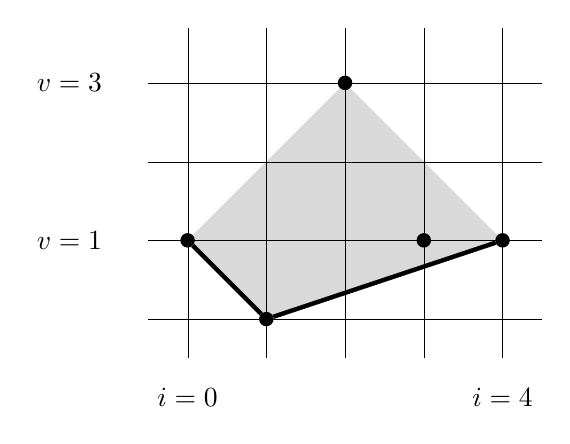
\begin{tikzpicture}[val/.style={circle, fill, draw, inner sep=1.7pt}]
		\fill[fill=gray!30] (0,1) -- (1,0) -- (4,1) -- (2,3) -- cycle;
		\node[val] (C0) at (0,1) {};
		\node[val] (C1) at (1,0) {};
		\node[val] (C2) at (2,3) {};
		\node[val] (C3) at (3,1) {};
		\node[val] (C4) at (4,1) {};
		\draw[ultra thick] (C0) -- (C1) -- (C4);
		\draw[step=1, line width=0.05pt] (-0.5, -0.5) grid (4.5, 3.7);
		\node at (0,-1) {$i=0$};  \node at (4,-1) {$i=4$};
		\node at (-1.5, 1) {$v=1$}; \node at (-1.5, 3) {$v=3$};
	\end{tikzpicture}\end{center}
	Poligon tersebut terdiri atas dua ruas garis dengan kemiringan $-1$ dan $\frac{1}{3}$.
\end{example}

\begin{theorem}\label{prop:Newton-polygon}
	Dengan notasi di atas, untuk setiap $s \in \R$,
	\[ \textbf{NP}(P)\; \text{memuat ruas garis dengan kemiringan $-s$} \iff \exists \lambda \in \overline{K}, \; P(\lambda)=0 \; \wedge \; v(\lambda)=s. \]
	Selain itu, panjang proyeksi pada sumbu $x$ dari ruas garis yang berkemiringan $-s$ sama dengan banyaknya akar di $\overline{K}$ yang memenuhi $v(\lambda)=s$ (dengan memperhitungkan multiplisitas).
\end{theorem}
\begin{proof}
	Tanpa mengurangi keumuman, andaikan $a_0 a_n \neq 0$. Setelah menggeser $\textbf{NP}(P)$ secara vertikal, kita dapat pula mengandaikan $a_n = 1$.	Daftarkan akar-akar $P$, yaitu $\lambda_1, \ldots, \lambda_n \in \overline{K}$ (dengan memperhitungkan multiplisitas), menurut valuasi yang meningkat:
	\[\begin{tikzcd}[column sep=small, row sep=small]
		v(\lambda_1) = \cdots = v(\lambda_{t_1}) \arrow[phantom, r, "=" description] & v_1 \arrow[sloped, phantom, d, "<" description] & (t_1 \;\text{akar}) \\
		v(\lambda_{t_1+1}) = \cdots = v(\lambda_{t_1 + t_2}) \arrow[phantom, r, "=" description] & v_2 \arrow[sloped, phantom, d, "<" description] & (t_2 \;\text{akar}) \\
		\vdots & \vdots & \vdots
	\end{tikzcd}\]
	Maka $v(a_n)=0$, dan untuk setiap $0 \leq k < n$ berlaku
	\[ v(a_{n-k}) = v\left( \sum_{1 \leq i_1 < \cdots < i_k \leq n} \lambda_{i_1} \cdots \lambda_{i_k} \right) \geq \min_{i_1 < \cdots < i_k}\left\{ v(\lambda_{i_1}) + \cdots + v(\lambda_{i_k}) \right\}. \]
	Jadi, untuk $0 \leq k \leq t_1$ berlaku $v(a_{n-k}) \geq k v_1$; selain itu, Lema \ref{prop:ultrametric} mengimplikasikan $v(a_{n-t_1}) = t_1 v_1$, sebab minimum ruas kanan dicapai tepat pada $(i_1, \ldots, i_{t_1}) = (1, \ldots, t_1)$. Jika $t_1=n$, hal ini menunjukkan bahwa $\textbf{NP}(P)$ hanya terdiri atas satu ruas garis dengan kemiringan $-v_1$. Jika $t_1 < n$, dengan cara yang sama diperoleh
	\[ 0 \leq k \leq t_2 \implies v(a_{n-t_1-k}) \geq t_1 v_1 + k v_2, \quad v(a_{n-t_1-t_2}) = t_1 v_1 + t_2 v_2. \]
	Dengan melanjutkan cara ini, dari kanan ke kiri $\textbf{NP}(P)$ dibentuk oleh ruas-ruas garis dengan kemiringan $-v_1 > -v_2 > \cdots$, yang panjang proyeksinya pada sumbu $x$ berturut-turut adalah $t_1, t_2, \ldots$, dan seterusnya.
\end{proof}

Lema K.\ Hensel merupakan contoh penerapan gagasan analisis dalam aljabar dan teori bilangan. Lema ini memiliki berbagai bentuk; di sini hanya satu bentuk yang diperkenalkan.
\begin{theorem}[Lema Hensel]\label{prop:Hensel-lemma}\index{Lema Hensel}
	Misalkan $K$ lengkap terhadap valuasi peringkat $1$ $v$, dan $P \in K^\circ[X]$. Jika $x_0 \in K^\circ$ memenuhi
	\[ v(P(x_0)) > 2v(P'(x_0)), \]
	dengan $P' \in K^\circ[X]$ turunan formal dari $P$ (Proposisi \ref{prop:polynomial-derivation}), maka terdapat $x \in K^\circ$ sedemikian sehingga $P(x) = 0$ dan
	\[ v(x - x_0) \geq v(P(x_0)) - v(P'(x_0)) > v(P'(x_0)). \]
	Pernyataan ketunggalan berikut juga berlaku: jika $x, x' \in K^\circ$ adalah akar-akar $P$, dan $v(x - x_0)$ serta $v(x' - x_0)$ keduanya $> v(P'(x_0))$, maka $x=x'$.
\end{theorem}
\begin{proof}
	Kita akan membangun barisan $x_0, x_1, \ldots$ di $K^\circ$ sedemikian sehingga untuk setiap $i \geq 0$ berlaku
	\begin{equation}\label{eqn:Hensel-sequence} \begin{gathered}
		v(P(x_{i+1})) \geq v(P(x_i)) + \underbracket{v(P(x_0)) - 2 v(P'(x_0))}_{>0}, \\
		v(P'(x_{i+1})) = v(P'(x_0)), \\
		v(x_{i+1} - x_i) \geq v(P(x_i)) - v(P'(x_0)).
	\end{gathered}\end{equation}
	Jika barisan seperti di atas telah diberikan, maka $v(P(x_i))$ meningkat tanpa batas atas, sehingga Proposisi \ref{prop:ultrametric-series} memberikan limit
	\[ x := \lim_{i \to \infty} x_i = x_0 + \sum_{i=0}^\infty (x_{i+1}-x_i)\; \in K^\circ, \qquad P(x)=0. \]
	Selain itu, $v(P(x_i)) \geq v(P(x_0))$ mengimplikasikan $v(x_{i+1} - x_i) \geq v(P(x_0)) - v(P'(x_0))$; dengan mengambil limit diperoleh $v(x - x_0) \geq \inf_{i \geq 0} v(x_{i+1} - x_i) \geq v(P(x_0)) - v(P'(x_0))$. Jadi $x$ memiliki semua sifat yang diinginkan. Selanjutnya kita membangun $(x_i)_{i \geq 0}$ secara rekursif, dimulai dari $x_0$.

	Andaikan $x_0, \ldots, x_i$ telah dibangun dan memenuhi \eqref{eqn:Hensel-sequence}, dengan $i \geq 0$. Berikut akan dijelaskan cara membangun $x_{i+1}$; gagasannya serupa dengan metode Newton. Perkenalkan peubah baru $Y$ dan tuliskan
	\[ P(X+Y) = P_0(X) + P_1(X) Y + P_2(X) Y^2 + \cdots, \quad P_k \in K^\circ[X]. \]
	Jelas bahwa $P_0 = P$ dan $P_1 = P'$. Syarat-syarat di atas mengimplikasikan $P_1(x_i) \neq 0$, sehingga kita dapat mengambil $t := -P(x_i)/P'(x_i)$; unsur ini memenuhi
	\begin{align*}
		v(t) & = v(P(x_i)) - v(P'(x_i)) = v(P(x_i)) - v(P'(x_0)), \\
		2v(t) & = v(P(x_i)) + v(P(x_i)) - 2v(P'(x_0)) \\
		& \geq v(P(x_i)) + v(P(x_0)) - 2v(P'(x_0)) > 0.
	\end{align*}
	Khususnya, $v(t) > 0$, sehingga $x_{i+1} := x_i + t \;\in K^\circ$. Pemilihan $t$ tersebut memberikan
	\begin{gather*}
		P(x_{i+1}) = P(x_i + t) = \sum_{2 \leq k \leq \deg P} P_k(x_i) t^k, \\
		v(P(x_{i+1})) \geq 2v(t) \geq v(P(x_i)) + v(P(x_0)) - 2v(P'(x_0)), \\
		v(x_{i+1} - x_i) = v(t) = v(P(x_i)) - v(P'(x_0)).
	\end{gather*}

	Dengan cara yang sama, dari ekspansi berkoefisien di $K^\circ$, yaitu $P'(X+Y) = P'(X) + P''_1(X) Y + \cdots$, diperoleh
	\[ P'(x_{i+1}) - P'(x_i) \in  t \cdot K^\circ, \quad v(P'(x_{i+1}) - P'(x_i)) \geq v(t). \]
	Namun $v(t) \geq v(P(x_0)) - v(P'(x_0)) > v(P'(x_0))$, sedangkan $v(P'(x_i)) = v(P'(x_0))$; Lema \ref{prop:ultrametric} segera memberikan $v(P'(x_{i+1})) = v(P'(x_i))$. Dengan demikian telah dibangun $x_0, \ldots, x_{i+1}$ yang memenuhi \eqref{eqn:Hensel-sequence}.

	Terakhir, kita buktikan ketunggalan. Perhatikan bahwa $x \in K^\circ$ dan $v(x-x_0) > v(P'(x_0))$ mengimplikasikan bahwa $P'(x) - P'(x_0) \in (x-x_0) K^\circ$ mempunyai valuasi lebih besar daripada $v(P'(x_0))$; maka Lema \ref{prop:ultrametric} memberikan $v(P'(x)) = v(P'(x_0))$. Sekarang ambil dua akar berbeda $x, x' \in K^\circ$ dari $P$. Terdapat $Q \in K^\circ[X]$ sedemikian sehingga $P(X) = (X-x)(X-x') Q(X)$. Oleh karena itu,
	\begin{gather*}
		P'(x) = (x-x')Q(x), \\
		v(P'(x)) \geq v(x-x') \geq \min\left\{ v(x - x_0), v(x' - x_0) \right\}.
	\end{gather*}
	Jika $v(x-x_0), v(x'-x_0) > v(P'(x_0))$, pengamatan tadi menghasilkan $v(P'(x_0)) \geq \cdots > v(P'(x_0))$, suatu kontradiksi.
\end{proof}

Kasus khusus yang paling umum adalah $v(P'(x_0))=0$, sebagai berikut. Tetapkan $\kappa := K^\circ/K^{\circ\circ}$ sebagai medan residu, dan tuliskan $x \mapsto \bar{x}$ untuk homomorfisme hasil bagi $K^\circ \twoheadrightarrow \kappa$. Setelah direduksi $\bmod \; K^{\circ\circ}$, setiap $Q \in K^\circ[X]$ dapat dievaluasi pada $\bar{x}$; hasilnya ditulis $Q(\bar{x})$, dan seterusnya.
\begin{corollary}\label{prop:Hensel-lemma-unique}
	Misalkan $K$ lengkap terhadap valuasi peringkat $1$ $v$, dan $P \in K^\circ[X]$. Jika $\bar{x}_0 \in \kappa$ memenuhi $P(\bar{x}_0) = 0$ dan $P'(\bar{x}_0) \neq 0$, maka terdapat tepat satu $x \in K^\circ$ sedemikian sehingga
	\[ \bar{x} = \bar{x}_0 \;\in \kappa, \qquad P(x)=0. \]
\end{corollary}
\begin{proof}
	Pilih sebarang $x_0 \mapsto \bar{x}_0$; syarat-syaratnya menjadi $v(P(x_0)) > 0$ dan $v(P'(x_0))=0$. Terapkan Teorema \ref{prop:Hensel-lemma}.
\end{proof}

Menyelesaikan persamaan di $\kappa$ jauh lebih mudah daripada di $K$; berikut sebuah contoh penting. Untuk setiap gelanggang komutatif $R$ dan bilangan bulat $m \neq 0$, definisikan grup perkalian $\mu_m(R) := \left\{ x \in R^\times: x^m = 1 \right\}$.

\begin{example}[Representan Teichmüller]\label{eg:Teichmuller-rep}
	Misalkan medan residu $\kappa$ dari $K$ memenuhi $\kappa \simeq \F_q$, dengan $q$ suatu pangkat dari bilangan prima $p$. Untuk bilangan bulat tak nol $m$, kita mempunyai homomorfisme grup
	\begin{align*}
		\mu_m(K) & \longrightarrow \mu_m(\kappa) \\
		x & \longmapsto x \bmod K^{\circ\circ}.
	\end{align*}
	Jika $p \nmid m$, homomorfisme di atas merupakan isomorfisme: perhatikan polinomial $P := X^m - 1 \in K^\circ[X]$. Setiap $\bar{x} \in \kappa^\times$ memenuhi $P'(\bar{x}) = m\bar{x}^{m-1} \neq 0$, sehingga Korolari \ref{prop:Hensel-lemma-unique} menunjukkan bahwa $\mu_m(K) \rightiso \mu_m(\kappa)$. Dalam kasus khusus $m = q-1$, diperoleh isomorfisme grup
	\[ \mu_{q-1}(K) \stackrel{\sim}{\longrightarrow} \mu_{q-1}(\kappa) = \kappa^\times. \]
	Unsur $x \in \mu_{q-1}(K)$ yang bersesuaian dengan $\bar{x} \in \kappa^\times$ disebut representan Teichmüller dari $\bar{x}$ di $K$. Untuk kemudahan, definisikan pula representan Teichmüller dari $0$ sebagai $0 \in K$; dengan demikian diperoleh pembenaman monoid perkalian $\kappa \hookrightarrow K^\circ$.
\end{example}

\begin{theorem}[M.\ Krasner]\label{prop:Krasner-lemma}
	Misalkan $K$ lengkap terhadap valuasi peringkat $1$ $v$. Tetapkan suatu penutupan separabel $K^\mathrm{sep} \subset \overline{K}$ dan ambil $x, y \in K^\mathrm{sep}$. Tuliskan $x = x_1, \ldots, x_n \in K^\mathrm{sep}$ untuk semua akar polinomial minimal $P_x \in K[X]$ dari $x$ (dengan kata lain, semua konjugat $x$). Jika
	\[ v(x-y) > v(x-x_i), \quad i=2, \ldots, n. \]
	maka $K(x) \subset K(y)$. Di sini kita memperluas $v$ ke $K^\mathrm{sep}$ menggunakan Korolari \ref{prop:valuation-ext-complete-alg}.
\end{theorem}
\begin{proof}
	Strateginya adalah membuktikan bahwa $x$ ditetapkan oleh setiap $\sigma \in \Gal(K^\text{sep}|K(y))$, lalu menyimpulkan $x \in K(y)$ dari korespondensi Galois (Teorema \ref{prop:infinite-Galois-corr}). Karena perluasan valuasi bersifat tunggal, untuk setiap $\sigma$ tersebut berlaku $v \circ \sigma = v$, sehingga
	\[ v(y-\sigma(x)) = v(\sigma(y-x)) = v(y-x) > v(x-x_i), \quad i=2, \ldots, n. \]
	Dengan demikian,
	\[ v(x-\sigma(x)) \geq \min\left\{ v(x-y), v(y-\sigma(x)) \right\}  > v(x-x_i), \quad i=2, \ldots, n. \]
	Karena terdapat $1 \leq j \leq n$ sedemikian sehingga $\sigma(x) = x_j$, pertidaksamaan di atas memaksa $j=1$, sehingga $\sigma(x)=x$.
\end{proof}

\begin{corollary}\label{prop:complete-alg-closed}
	Misalkan $|\cdot|$ adalah nilai mutlak pada medan tertutup separabel (atau tertutup aljabar) $K$. Maka pelengkapan terkait $\hat{K}$ juga merupakan medan tertutup separabel (atau tertutup aljabar).
\end{corollary}
Ingat bahwa $K$ disebut tertutup separabel apabila penutup separabelnya di dalam $\overline{K}$ sama dengan $K$ sendiri; jika $\text{char}(K)=0$, hal ini ekuivalen dengan tertutup aljabar.

\begin{proof}
	Jika $|\cdot|$ adalah nilai mutlak Archimedes, Teorema \ref{prop:archimedean-complete-field} mengimplikasikan $\hat{K}=\R$ atau $\CC$; kasus pertama akan memberikan $\Q \subset K \subset \R$, yang mustahil bagi medan tertutup aljabar. Maka selanjutnya kita dapat mengandaikan bahwa $|\cdot|$ non-Archimedes, yang bersesuaian dengan suatu valuasi peringkat $1$ pada $K$. Untuk kasus medan tertutup separabel, ambil $x \in \hat{K}^{\text{sep}}$. Karena $K$ rapat di $\hat{K}$, kita dapat memilih polinomial monik $P \in K[X]$ yang koefisien-koefisiennya cukup dekat dengan koefisien-koefisien $P_x$; dengan demikian $|P(x)|=|P(x)-P_x(x)|$ dapat dibuat sekecil yang diinginkan. Dengan meninjau diskriminan polinomial (Contoh \ref{eg:polynomial-discriminant}), $P$ tidak mempunyai akar ganda sebagaimana $P_x$. Karena itu $P$ terurai menjadi faktor-faktor linear, dan terdapat akar $y \in K$ dengan $|y-x|$ cukup kecil. Teorema \ref{prop:Krasner-lemma} segera memberikan $\hat{K}(x) \subset \hat{K}(y) = \hat{K}$.

	Untuk kasus medan tertutup aljabar, kita boleh mengandaikan $\text{char}(K) = p > 0$. Ambil $x \in \overline{\hat{K}}$ dan tuliskan polinomial minimalnya atas $\hat{K}$ dalam bentuk $P_x(X) = P_x^\flat(X^{p^m})$, dengan $P_x^\flat$ tanpa akar ganda. Jadi $y := x^{p^m} \in \hat{K}^{\text{sep}}$; dari langkah sebelumnya, $\hat{K}^{\text{sep}} = \hat{K}$. Maka terdapat barisan titik $y_1, y_2, \ldots$ di $K$ dengan $|y_k - y| \to 0$. Jelas bahwa $\left| y_k^{p^{-m}} - y^{p^{-m}} \right| \to 0$, sehingga $x = y^{p^{-m}} \in \hat{K}$. Ini membuktikan pernyataan tersebut.
\end{proof}

\section{Vektor Witt}\label{sec:Witt-vector}
Sepanjang bagian ini, tetapkan sebuah bilangan prima $p$.

Pertama-tama kita ingat kembali struktur gelanggang bilangan bulat $p$-adik $\Z_p$. Karena $\Z_p/p\Z_p$ dapat diidentifikasi dengan $\F_p$, kita dapat memilih suatu pemetaan $\tau: \F_p \to \Z_p$ yang memenuhi $\tau(x) \equiv x \pmod {p\Z_p}$; $\tau(x)$ disebut suatu pengangkatan dari $x$. Ambil $\tilde{x} \in \Z_p$, dan tuliskan $x$ untuk citranya di $\F_p$. Maka terdapat $\tilde{x}_1 \in \Z_p$ sedemikian sehingga $\tilde{x} = \tau(x) + p \tilde{x}_1$; karena $p$ bukan pembagi nol, $\tilde{x}_1$ tunggal. Dengan mengulangi proses ini, kita memperoleh $\tilde{x}_1 = \tau(x_1) + p\tilde{x}_2$, dan seterusnya. Dengan demikian diperoleh barisan tunggal $x_0, x_1, \ldots$ di $\F_p$ sedemikian sehingga, untuk $n \geq 0$,
\[ \tilde{x} = \tau(x_0) + \tau(x_1) p + \cdots + \tau(x_n) p^n + \tilde{x}_{n+1} p^{n+1}, \quad \tilde{x}_{n+1} \in \Z_p. \]
Deret tak hingga $\sum_{n=0}^\infty \tau(x_n) p^n$ konvergen ke $\tilde{x}$ di $\Z_p$. Sebaliknya, menurut Proposisi \ref{prop:ultrametric-series}, setiap barisan $\left( x_n \in \F_p \right)_{n \geq 0}$ menentukan $\tilde{x} := \sum_{n=0}^\infty \tau(x_n) p^n \in \Z_p$. Jadi diperoleh bijeksi himpunan
\begin{align*}
	\prod_{n \geq 0} \F_p & \stackrel{1:1}{\longrightarrow} \Z_p \\
	(x_n)_{n \geq 0} & \longmapsto \sum_{n=0}^\infty \tau(x_n) p^n.
\end{align*}
Deskripsi ini memang sederhana, tetapi menyisakan dua pertanyaan:
\begin{compactitem}
	\item Bijeksi tersebut bergantung pada pilihan pengangkatan $x \mapsto \tau(x)$; adakah pilihan yang kanonik dan mudah digunakan?
	\item Bagaimana struktur gelanggang $\Z_p$ tercermin pada $\prod_{n \geq 0} \F_p$?
\end{compactitem}
Untuk pertanyaan pertama, Contoh \ref{eg:Teichmuller-rep} memberikan pemetaan baku $\tau: \F_p \to \Z_p$ yang sekaligus merupakan homomorfisme monoid perkalian. Untuk menjawab pertanyaan kedua secara lengkap, sebaiknya kita memperluas sudut pandang.

\begin{definition}\index{aljabar!sempurna}
	Misalkan $\kappa$ suatu aljabar-$\F_p$ komutatif. Jika $\Frob_p: x \mapsto x^p$ adalah automorfisme dari $\kappa$, maka $\kappa$ disebut \emph{sempurna}.
\end{definition}
Ini merupakan perluasan alami dari kasus medan; lihat Teorema \ref{prop:perfect-field-char}. Definisi \ref{def:Frob-aut} juga melibatkan pemetaan serupa.

\begin{definition}\label{def:p-ring} \index{gelanggang-p-ketat@gelanggang $p$ ketat (strict $p$-ring)}
	Misalkan $A$ suatu gelanggang komutatif, dan diberikan rantai menurun ideal $\mathfrak{a}_1 \supset \mathfrak{a}_2 \supset \cdots$ sedemikian sehingga
	\begin{compactitem}
		\item topologi yang bersesuaian menjadikan $A$ gelanggang topologis Hausdorff yang lengkap (lihat Catatan \ref{rem:ring-completion}), yakni $A \rightiso \varprojlim_n A/\mathfrak{a}_n$;
		\item untuk setiap $n, m$ berlaku $\mathfrak{a}_n \mathfrak{a}_m \subset \mathfrak{a}_{n+m}$;
		\item $p \in \mathfrak{a}_1$, dan gelanggang residu $\kappa := A/\mathfrak{a}_1$ sempurna.
	\end{compactitem}
	Kita menyebut $A$, bersama data-data ini, suatu gelanggang-$p$. Jika selain itu $p$ bukan pembagi nol di $A$ dan $\mathfrak{a}_n = p^n A$, maka $A$ disebut gelanggang-$p$ ketat.
\end{definition}
Sebagai contoh, $\Z_p$ adalah gelanggang-$p$ ketat, sedangkan aljabar-$\F_p$ $\F_p \llbracket t \rrbracket$, dengan $\mathfrak{a}_n := (t^n)$, merupakan gelanggang-$p$ tetapi jelas tidak ketat.

\begin{lemma}\label{prop:aux-p-power}
	Misalkan gelanggang komutatif $A$ memiliki rantai menurun ideal $\mathfrak{a}_1 \supset \mathfrak{a}_2 \supset \cdots$ sedemikian sehingga $\mathfrak{a}_n \mathfrak{a}_m \subset \mathfrak{a}_{n+m}$ dan $p \in \mathfrak{a}_1$. Maka untuk setiap $a,b \in A$ berlaku
	\[ a \equiv b \pmod{\mathfrak{a}_m} \implies a^{p^n} \equiv b^{p^n} \pmod{\mathfrak{a}_{m+n}}. \]
\end{lemma}
Hasil ini dapat dikatakan sebagai poros bagi semua argumen dalam bagian ini; dalam penerapan, kasus yang sering diambil adalah $\mathfrak{a}_n = p^n A$.
\begin{proof}
	Kita segera mereduksi ke kasus $n=1$. Selanjutnya, tetapkan $P(X,Y) := \frac{X^p-Y^p}{X-Y} \in \Z[X,Y]$. Syarat di atas mengimplikasikan $P(a,b) \equiv P(a,a) \equiv pa^{p-1} \pmod{\mathfrak{a}_m}$, sehingga $a^p - b^p = (a-b) P(a,b)$ berada di dalam $\mathfrak{a}_m (pA + \mathfrak{a}_m) \subset \mathfrak{a}_{m+1}$. Selesai.
\end{proof}

\begin{proposition}\label{prop:Teichmuller-lift}\index{pengangkatan Teichmüller}
	Misalkan $A$ suatu gelanggang-$p$ dan $\kappa := A/\mathfrak{a}_1$. Maka terdapat tepat satu pemetaan $\tau: \kappa \to A$ sedemikian sehingga
	\begin{compactitem}
		\item citra $\tau(x)$ di $\kappa$ adalah $x$;
		\item $\tau$ bersifat multiplikatif: $\tau(1)=1$, $\tau(xy)=\tau(x)\tau(y)$.
	\end{compactitem}
	Pemetaan $\tau$ disebut pengangkatan Teichmüller. Jika $A$ merupakan aljabar-$\F_p$, maka $\tau$ juga bersifat aditif: $\tau(x+y)=\tau(x)+\tau(y)$.
\end{proposition}
\begin{proof}
	Karena $\kappa$ sempurna, untuk $x \in \kappa$ dan setiap $n \geq 0$ terdapat akar ke-$p^n$ tunggal $x^{p^{-n}} \in \kappa$; pilih sebarang prapeta $\left[ x^{p^{-n}} \right]$ di $A$. Kita ingin mendefinisikan
	\[ \tau(x) := \lim_{n \to \infty} \left[ x^{p^{-n}} \right]^{p^n}. \]
	Jika $n \geq m$, maka $\left[ x^{p^{-n}} \right]^{p^{n-m}}$ merupakan suatu prapeta dari $x^{p^{-m}}$; tanpa mengurangi keumuman, kita tuliskan prapeta itu sebagai $\left[ x^{p^{-m}} \right]$. Lema \ref{prop:aux-p-power} mengimplikasikan
	\[ \left[ x^{p^{-n}} \right]^{p^n} = \left[ x^{p^{-m}} \right]^{p^m} \;\text{memiliki citra di}\; A/\mathfrak{a}_{m+1}\; \text{yang hanya bergantung pada}\; x^{p^{-m}} \in \kappa \]
	Karena $A$ lengkap, hal ini menunjukkan bahwa limit yang mendefinisikan $\tau$ memang ada dan hanya bergantung pada $x$. Jelas bahwa $\tau(x) \equiv x \pmod{\mathfrak{a}_1}$.

	Sifat $(xy)^{p^{-n}} = x^{p^{-n}} y^{p^{-n}}$ mengimplikasikan kemultiplikatifan $\tau$. Selain itu, setiap pengangkatan multiplikatif $\tau': \kappa \to A$ memenuhi $\tau'( x^{p^{-n}})^{p^n} = \tau'(x)$; dengan mengambil $\left[ \cdots \right] = \tau'(\cdots)$ dalam argumen sebelumnya, diperoleh ketunggalan $\tau=\tau'$. Terakhir, jika $A$ merupakan aljabar-$\F_p$, konstruksi di atas bersama identitas $\tilde{x}^p + \tilde{y}^p = (\tilde{x}+\tilde{y})^p$ di $A$ menjamin keaditifan $\tau$.
\end{proof}

Misalkan $A$ suatu gelanggang-$p$ ketat dan $\kappa := A/pA$. Sekarang metode yang digunakan untuk $\Z_p$ pada awal bagian ini dapat diterapkan tanpa perubahan, sehingga diperoleh bijeksi himpunan yang kanonik
\begin{equation}\label{eqn:Witt-bijection}\begin{aligned}
	\prod_{n \geq 0} \kappa & \stackrel{1:1}{\longrightarrow} A \\
	(x_n)_{n \geq 0} & \longmapsto \sum_{n=0}^\infty \tau\left( x_n^{p^{-n}} \right) p^n.
\end{aligned}\end{equation}
Unsur nol dan unsur satu dari gelanggang $A$ jelas bersesuaian dengan $(0,0,\ldots)$ dan $(1, 0, \ldots)$. Perhatikan bahwa jika $\kappa = \F_p$, selalu berlaku $x^{p^{-n}} = x$. Manfaat cerdik dari penggunaan $x^{p^{-n}}$ akan tampak dalam pembuktian berikutnya.

Kita ingin menyelidiki bagaimana struktur gelanggang $A$ ditarik balik ke $\prod_{n \geq 0} \kappa$. Gelanggang yang bersesuaian akan ditulis $\WittV(\kappa)$ untuk membedakannya dari hasil kali langsung. Sebagai contoh, untuk penjumlahan tuliskan
\[ \sum_{n \geq 0} \tau\left( S_n(x_0, \ldots, y_0, \ldots)^{p^{-n}} \right) p^n = \sum_{n \geq 0} \tau(x_n^{p^{-n}}) p^n + \sum_{n \geq 0} \tau(y_n^{p^{-n}}) p^n, \]
bagaimana kita mendeskripsikan $S_n$? Pertama-tama, dengan mereduksi kedua ruas persamaan di atas modulo $pA$, diperoleh $S_0 = x_0 + y_0 \in \kappa$. Untuk mendeskripsikan $S_1$, kita harus meninjau
\[ \tau(x_0 + y_0) + \tau( S_1^{p^{-1}} )p \equiv \tau(x_0) + \tau(y_0) + \left( \tau(x_1^{p^{-1}}) + \tau(y_1^{p^{-1}}) \right)p \pmod{p^2 A}. \]
Bagaimana menentukan $\tau(x_0) + \tau(y_0) - \tau(x_0+y_0)\; \bmod p^2 A$? Kuncinya adalah mengingat kembali dari pembuktian Proposisi \ref{prop:Teichmuller-lift} bahwa
\begin{equation}\label{eqn:Teich-lifting-power}
	\tau(z) \equiv \left[ z^{p^{-n}} \right]^{p^n} \pmod{ p^{n+1} A}, \quad z \in \kappa,
\end{equation}
dengan $[\cdots]$ sebarang prapeta. Lema \ref{prop:aux-p-power} memberikan $[x^{1/p} + y^{1/p}]^p \equiv \left( [x^{1/p}] + [y^{1/p}] \right)^p \pmod {p^2 A}$. Karena $p \in A$ bukan pembagi nol, dari kekongruenan modulo $p^2 A$ kita memperoleh
\begin{align*}
	S_1^{p^{-1}} & = x_1^{1/p} + y_1^{1/p} + \frac{1}{p} \left( \left[ x_0^{1/p} \right]^p + \left[ y_0^{1/p} \right]^p - \left[ x_0^{1/p} + y_0^{1/p} \right]^p \right) \bmod pA \\
	& = x_1^{1/p} + y_1^{1/p} - \sum_{0 < k < p} \frac{1}{p} \binom{p}{k} \left[ x_0^{1/p} \right]^k \left[ y_0^{1/p} \right]^{p-k} \bmod pA.
\end{align*}
Dengan menerapkan $z \mapsto z^p$ pada kedua ruas dan menggunakan $\left[ z^{1/p} \right]^p \equiv z \pmod {pA}$, diperoleh
\[ S_1 = x_1 + y_1 - \sum_{0 < k < p} \frac{1}{p} \binom{p}{k} x_0^k y_0^{p-k}. \]
Bentuk suku-suku yang lebih tinggi $S_2, S_3, \ldots$ lebih rumit, tetapi algoritmanya jelas. Dari sini mudah dilihat bahwa
\begin{compactitem}
	\item penjumlahan dan perkalian pada gelanggang $A$ tercermin pada $\WittV(\kappa)$ dan diberikan per komponen oleh keluarga polinomial $S_n$, $P_n$;
	\item bentuk keluarga polinomial ini tidak bergantung pada $A$ maupun $\kappa$, dan secara rekursif dapat dituliskan sebagai polinomial berkoefisien bulat.
\end{compactitem}
Hal ini mengisyaratkan bahwa struktur gelanggang-$p$ ketat seharusnya memiliki suatu sifat universal. Karya E.\ Witt \cite{Witt37} menyelesaikan persoalan-persoalan ini dengan gemilang. Namun, untuk membangun $S_n, P_n$, kita harus meninjau kasus komponen $x_i$ yang bernilai dalam gelanggang komutatif umum $R$ dan menyelidiki gelanggang Witt terkait $\WittV(R)$. Jalan memutar ini bukan hanya perlu, melainkan justru merupakan inti karya Witt.

Uraian berikut mengikuti pendekatan \cite[\S 1]{Hess15}; perbedaannya adalah bahwa artikel tersebut menangani semua bilangan prima $p$ sekaligus dan memperoleh gelanggang yang disebut gelanggang Witt besar.

\begin{definition}
	Misalkan $R$ suatu gelanggang komutatif. Definisikan $\WittV(R) := \prod_{i \geq 0} R$, dan untuk setiap $n \geq 0$ definisikan pemetaan
	\begin{align*}
		w_n: \WittV(R) & \longrightarrow R \\
		x = (x_j)_{j \geq 0} & \longmapsto w_n(x_0, \ldots, x_n) = \sum_{i=0}^n x_i^{p^{n-i}} p^i.
	\end{align*}
	Selanjutnya, definisikan $w: \WittV(R) \to \prod_{n \geq 0} R$ dengan $w(x) := (w_0(x), w_1(x), w_2(x), \ldots)$.
\end{definition}
Secara tradisional, $w_n(x)$ disebut komponen bayangan ke-$n$ dari $x$ (bahasa Jerman: \textit{die Geisterkomponente}), sebab dalam persoalan awal kita, $R=\kappa$ selalu merupakan aljabar-$\F_p$, sehingga $w_n(x)$ menyusut menjadi $x_0^{p^n}$; namun kunci untuk membuka rahasia $\WittV(\kappa)$ justru terletak pada ``bayangan'' yang tersisa. Ada pula beberapa pengamatan berikut:
\begin{compactitem}
	\item Untuk setiap homomorfisme gelanggang komutatif $\phi: R \to S$, terdapat pemetaan terkait $\WittV(\phi): \WittV(R) \to \WittV(S)$ yang memetakan $(x_i)_i$ ke $(\phi(x_i))_i$.
	\item Kodomain $\prod_{i \geq 0} R$ dari pemetaan $w$ mempunyai struktur gelanggang hasil kali langsung (Definisi \ref{def:ring-direct-product}), yakni operasi gelanggang dilakukan komponen demi komponen.
	\item Gelanggang $R$ disebut bebas torsi-$p$ jika $pr =0 \iff r=0$ untuk setiap $r \in R$. Di bawah syarat bebas torsi-$p$, $x_0, \ldots, x_n$ dapat dipulihkan berturut-turut dari $w_0, \ldots, w_n$, sehingga $w$ injektif. \index{bebas torsi-$p$ ($p$-torsion free)}
\end{compactitem}

Tugas berikutnya adalah memberikan struktur gelanggang alami pada $\WittV(R)$. Karena sebagai himpunan gelanggang Witt $\WittV(R)$ sama dengan $R \times R \times \cdots$, unsur-unsur $\WittV(R)$ disebut vektor Witt\index{vektor Witt}. Kita memerlukan sebuah lema yang mudah digunakan.
\begin{lemma}[B.\ Dwork]\label{prop:Dwork-Witt}
	Andaikan terdapat homomorfisme gelanggang $\phi_p: R \to R$ sedemikian sehingga $\phi_p(r) \equiv r^p \pmod {pR}$. Maka citra $w$ sama dengan
	\[ \left\{ (r_n)_{n \geq 0} \in \prod_{n \geq 0} R : \quad \forall n \geq 1, \; r_n \equiv \phi_p(r_{n-1}) \pmod {p^n R}  \right\}. \]
\end{lemma}
\begin{proof}
	Karena $\phi_p$ homomorfisme gelanggang, untuk $n \geq 1$ Lema \ref{prop:aux-p-power} memberikan
	\[ \phi_p(w_{n-1}(x)) = \sum_{i < n} \phi_p(x_i)^{p^{n-1-i}} p^i \equiv \sum_{i < n} x_i^{p^{n-i}} p^i \pmod {p^n R}. \]
	Jadi memang $w_n(x) \equiv \phi_p(w_{n-1}(x)) \pmod {p^n R}$. Sebaliknya, diberikan barisan $r_0, r_1, \ldots \in R$ yang memenuhi $r_n \equiv \phi_p(r_{n-1}) \pmod {p^n R}$, kita membangun secara rekursif $x_0 := r_0, \ldots, x_{n-1} \in R$ dan mengandaikan $i < n \implies w_i((x_0, \ldots, x_i)) = r_i$. Maka argumen sebelumnya memberikan
	\[ r_n - \sum_{i < n} x_i^{p^{n-i}} p^i \equiv r_n - \phi_p(w_{n-1}(x)) \equiv 0 \pmod {p^n R}, \]
	sehingga terdapat $x_n \in R$ sedemikian sehingga $r_n = \sum_{i<n} x_i^{p^{n-i}} p^i + x_n p^n$, yakni $r_n = w_n(x_0, \ldots, x_n)$.
\end{proof}
Dengan demikian, di bawah syarat-syarat lema tersebut segera tampak bahwa $\Image(w)$ merupakan subgelanggang dari $\prod_{i \geq 0} R$.

\begin{theorem}\label{prop:Witt-ring}\index{gelanggang Witt}
	Pada semua $\WittV(R)$ terdapat tepat satu keluarga struktur gelanggang komutatif sedemikian sehingga $w: \WittV(R) \to \prod_{n \geq 0} R$ merupakan homomorfisme gelanggang, $(0, 0, \ldots)$ merupakan unsur nol, $(1, 0, \ldots)$ merupakan unsur satu, dan:
	\begin{itemize}
		\item untuk setiap homomorfisme gelanggang $\phi: R \to S$, diagram berikut komutatif di $\cate{CRing}$:
		\[\begin{tikzcd}
		\WittV(R) \arrow[d, "w"'] \arrow[r, "\WittV(\phi)"] & \WittV(S) \arrow[d, "w"] \\
		\prod_{n \geq 0} R \arrow[r, "\prod_n \phi"'] & \prod_{n \geq 0} S
		\end{tikzcd}\]
		\item Terdapat keluarga polinomial yang ditentukan secara tunggal, $S_n \in \Z[X_0, \ldots, Y_0, \ldots]$, $P_n \in \Z[X_0, \ldots, Y_0, \ldots]$, dan $M_n \in \Z[X_0, \ldots, X_n]$, sedemikian sehingga struktur gelanggang $\WittV(R)$ ditentukan oleh
		\begin{align*}
			(x_n)_{n \geq 0} + (y_n)_{n \geq 0} & = (S_n(x_0, \ldots, x_n, y_0, \ldots, y_n))_{n \geq 0}, \\
			(x_n)_{n \geq 0} \cdot (y_n)_{n \geq 0} & = (P_n(x_0, \ldots, x_n, y_0, \ldots, y_n))_{n \geq 0}, \\
			-(x_n)_{n \geq 0} & = (M_n(x_0, \ldots, x_n))_{n \geq 0}
		\end{align*}
		dan polinomial-polinomial ini tidak bergantung pada $R$.
	\end{itemize}
	Dengan demikian, $\WittV(\cdot)$ memberikan suatu funktor dari kategori gelanggang komutatif $\cate{CRing}$ ke dirinya sendiri.
\end{theorem}
\begin{proof}
	Diberikan $(x_i)_i, (y_i)_i \in \WittV(R)$, untuk mendefinisikan operasi gelanggang yang alami di antara keduanya (yakni funktorial dalam $R$), pertama-tama ambil $x_i := X_i$ dan $y_i := Y_i$ sebagai peubah bebas, serta $R := \Z[X_0, \ldots, Y_0, \ldots]$. Menurut sifat universal gelanggang polinomial, terdapat endomorfisme $\phi_p: R \to R$ sedemikian sehingga
	\[ \phi_p(X_n) = X_n^p, \quad \phi_p(Y_n) = Y_n^p, \]
	dan bersama Teorema Kecil Fermat (Catatan \ref{rem:Fermat-little}) diperoleh $\forall r \; \phi_p(r) = r^p \pmod{pR}$. Lema \ref{prop:Dwork-Witt} menjamin bahwa unsur-unsur gelanggang $\prod_{n \geq 0} R$
	\[ w(x) + w(y), \quad w(x)w(y), \quad -w(x) \]
	tetap berada di $\Image(w)$. Karena $R$ bebas torsi-$p$, prapeta-prapeta mereka di bawah $w$ tunggal; masing-masing kita tulis $(S_i)_i, (P_i)_i, (M_i)_i$ (untuk menangani $M_i$, gunakan gelanggang $\Z[X_0, X_1, \ldots]$). Dari pembuktian lema juga diketahui bahwa $S_i, P_i, M_i$ hanya melibatkan peubah $X_0, \ldots, X_i$ dan $Y_0, \ldots, Y_i$. Kita mengklaim bahwa untuk gelanggang umum $R$, polinomial-polinomial berkoefisien bulat ini menjadikan $\WittV(R)$ suatu gelanggang komutatif:
	\begin{gather*}
		(x_i)_i + (y_i)_i = (S_i(x,y))_i, \quad (x_i)_i (y_i)_i = (P_i(x,y))_i, \quad  -(x_i)_i = (M_i(x))_i, \\
		0_{\WittV(R)} = (0,0, \ldots), \quad 1_{\WittV(R)} = (1,0,\ldots).
	\end{gather*}
	Sebagai contoh, untuk penjumlahan gunakan homomorfisme dari $\Z[X_0, \ldots, Y_0, \ldots]$ ke $R$,
	$\begin{tikzcd}[row sep=0pt, column sep=small] X_i \arrow[mapsto, r] & x_i \\ Y_i \arrow[mapsto, r] & y_i \end{tikzcd}$,
	Definisi di atas untuk peubah bebas menunjukkan bahwa diagram
	\[\begin{tikzcd}
		\WittV(R) \times \WittV(R) \arrow[d, "{(S_i)_i}"'] \arrow[r, "{(w,w)}"] & \prod_{i \geq 0} R  \times \prod_{i \geq 0} R \arrow[d, "+"] \\
		\WittV(R) \arrow[r, "w"'] & \prod_{i \geq 0} R
	\end{tikzcd}\]
	komutatif. Jika $R$ bebas torsi-$p$, maka $w$ injektif, dan $w(0_{\WittV(R)}) = (0, \ldots, 0)$; jadi sifat-sifat seperti komutativitas, asosiativitas, dan unsur nol diwarisi dari $\prod_{i \geq 0} R$. Untuk $R$ umum, tetapkan suatu keluarga pembangkit $\mathcal{X} \subset R$ dan bentuk gelanggang polinomial $R' := \Z[\mathcal{X}]$. Terdapat surjeksi terkait $R' \twoheadrightarrow R$ dan $\WittV(R') \twoheadrightarrow \WittV(R)$. Karena $R'$ bebas torsi-$p$, aksioma-aksioma gelanggang untuk $\WittV(R)$ tetap dapat direduksi menjadi pemeriksaan pada $\WittV(R')$.

	Dengan cara yang sama dapat dibuktikan bahwa untuk setiap homomorfisme gelanggang $\phi: R \to S$, pemetaan $\WittV(\phi): \WittV(R) \to \WittV(S)$ merupakan homomorfisme gelanggang. Argumen ini juga menunjukkan ketunggalan struktur gelanggang yang diminta.
\end{proof}

Karena $S_n$, $P_n$, dan $M_n$ hanya melibatkan peubah $X_0, \ldots, X_n$ dan $Y_0, \ldots, Y_n$, kita dapat mendefinisikan gelanggang Witt terpangkas \index[sym1]{Witt@$\WittV(R)$, $\WittV_n(R)$}
\[ \WittV_n(R)  := \left\{ (x_0, \ldots, x_{n-1}) : x_i \in R \right\}. \]
Gelanggang ini tetap memiliki pemetaan $w_i: \WittV_n(R) \to R$ ($0 \leq i < n$), dan terdapat homomorfisme gelanggang alami $\WittV(\cdot) \to \WittV_n(\cdot)$ serta $\WittV_{n+1}(\cdot) \to \WittV_n(\cdot)$ (yakni ``pemangkasan''), dan seterusnya. Pembaca dipersilakan memeriksa bahwa gelanggang $\WittV_1(R)$ sebenarnya sama dengan $R$.

Pada gelanggang Witt terdapat pula beberapa operasi sederhana tetapi amat penting berikut ini.
\begin{enumerate}
	\item Pergeseran (bahasa Jerman: \textit{die Verschiebung}) $V: \WittV(R) \to \WittV(R)$, yang memetakan $(x_0, x_1, \ldots)$ ke $(0, x_0, x_1, \ldots)$. Jelas bahwa $V$ bersifat funktorial: untuk setiap homomorfisme gelanggang $\phi: R \to S$, berlaku $V \circ \WittV(\phi) = \WittV(\phi) \circ V$. Berikut ditunjukkan bahwa $V$ sebenarnya adalah homomorfisme grup aditif; jelas bahwa diagram berikut komutatif:
		\[\begin{tikzcd}
			\WittV(R) \arrow[r, "w"] \arrow[d, "V"'] & \prod_{n \geq 0} R \arrow[d, "{V^w}"] & (y_i)_{i \geq 0} \arrow[phantom, l, "\ni" description] \arrow[mapsto, d] \\
			\WittV(R) \arrow[r, "w"'] & \prod_{n \geq 0} R & (0, py_0, py_1, \ldots) \arrow[phantom, l, "\ni" description]
		\end{tikzcd}\]
		Jelas bahwa $V^w$ merupakan homomorfisme grup aditif. Jika $R$ bebas torsi-$p$, maka $w$ merupakan monomorfisme, sehingga $V$ juga bersifat aditif; untuk $R$ umum, gunakan cara dalam pembuktian Teorema \ref{prop:Witt-ring}.
	\item Homomorfisme Frobenius $F: \WittV(R) \to \WittV(R)$. Homomorfisme ini dicirikan sebagai keluarga homomorfisme yang funktorial dalam $R$ dan membuat diagram berikut komutatif:
		\[\begin{tikzcd}
			\WittV(R) \arrow[r, "w"] \arrow[d, "F"'] & \prod_{n \geq 0} R \arrow[d, "{F^w}"] & (y_i)_{i \geq 0} \arrow[phantom, l, "\ni" description] \arrow[mapsto, d] \\
			\WittV(R) \arrow[r, "w"'] & \prod_{n \geq 0} R & (y_1, y_2, \ldots) \arrow[phantom, l, "\ni" description]
		\end{tikzcd} \]
		Pembuktiannya sama dengan pembuktian Teorema \ref{prop:Witt-ring}. Pertama, tinjau unsur berkomponen peubah bebas $(X_i)_{i \geq 0} \in \WittV(\Z[X_0, \ldots])$, dan perhatikan bahwa gelanggang $\Z[X_0, \ldots]$ dilengkapi endomorfisme $\phi_p: X_i \mapsto X_i^p$ yang memenuhi $\phi_p(x) \equiv x^p \pmod p$. Terapkan Lema \ref{prop:Dwork-Witt} untuk menunjukkan bahwa $F^w(w(X_0, X_1, \ldots)) \in \Image(w)$; prapeta tunggalnya ditulis $(F_i(X_0, X_1, \ldots))_{i \geq 0} \in \WittV(\Z[X_0, \ldots])$. Ini mendefinisikan $F(x_0, x_1, \ldots) = (F_i(x_0, x_1, \ldots))_{i \geq 0}$ untuk setiap gelanggang $R$. Untuk membuktikan bahwa $F$ homomorfisme gelanggang, cukup perhatikan bahwa $F^w$ juga homomorfisme gelanggang, lalu ulangi teknik dalam pembuktian Teorema \ref{prop:Witt-ring}. Funktorialitas dibuktikan dengan cara yang sama.
	\item Pengangkatan Teichmüller $\tau: R \to \WittV(R)$, yang memetakan $x$ ke $(x,0,0, \ldots)$. Pemetaan ini jelas juga funktorial dalam $R$, dan terdapat diagram komutatif
		\[\begin{tikzcd}[column sep=tiny]
			& R \arrow[ld, "\tau"'] \arrow[rd, "\tau^w"] & x \arrow[phantom, l, "\ni" description] \arrow[mapsto, rd] & \\
			\WittV(R) \arrow[rr, "w"'] & & \prod_{n \geq 0} R & (x^{p^i})_{i \geq 0} \arrow[phantom, l, "\ni" description]
		\end{tikzcd}\]
		Jelas bahwa $\tau^w$ merupakan homomorfisme monoid perkalian. Dengan argumen di atas, kita mereduksi ke kasus bebas torsi-$p$ dan memperoleh bahwa $\tau$ juga bersifat multiplikatif, $\tau(xy)=\tau(x)\tau(y)$, serta $\tau(1) = (1,0, \ldots) = 1_{\WittV(R)}$.
\end{enumerate}

Selain itu, $\Ker[ \WittV(\cdot) \twoheadrightarrow \WittV_n(\cdot)] = \Image(V^n)$; khususnya, $\Image(V^n)$ adalah suatu ideal. Pemetaan $V$ juga dapat didefinisikan pada versi terpangkas $\WittV_n(\cdot)$ dan memberikan barisan eksak pendek grup aditif
\begin{equation}\label{eqn:Witt-V}\begin{tikzcd}[row sep=tiny]
	0 \arrow[r] & \WittV_n(\cdot) \arrow[r, "V^r"] & \WittV_{n+r}(\cdot) \arrow[r, "(\text{pemangkasan})^n"] & \WittV_r(\cdot) \arrow[r] & 0 \\
	& (x_0, \ldots, x_{n-1}) \arrow[mapsto, r] & (0, \ldots, 0, x_0, \ldots, x_{n-1}) & & \\
	& & (y_0, \ldots, y_{n+r-1}) \arrow[mapsto, r] & (y_0, \ldots, y_{r-1}) &
\end{tikzcd}\end{equation}
Singkatnya, baik $\WittV(R)$, $\WittV_n(R)$, maupun homomorfisme dan operasi di antara mereka seperti $V$ dan $F$, semuanya funktorial dalam gelanggang $R$. Jika hanya struktur grup aditif dari $\WittV(R)$ dan $\WittV_n(R)$ yang ditinjau, maka yang telah kita bangun sesungguhnya adalah keluarga funktor grup dalam arti Definisi \ref{def:group-functor}, beserta morfisme-morfisme di antara mereka seperti $\WittV(\cdot) \to \WittV_n(\cdot)$, $V$, dan $F$. Hal ini sangat penting bagi penerapan dalam geometri aljabar aritmetika; semuanya merupakan titik awal teori modul Dieudonné.

\begin{lemma}\label{prop:Frob-Witt-char-p}
	Tuliskan $(F(x)_i)_{i \geq 0}$ untuk citra $(x_i)_{i \geq 0} \in \WittV(R)$ di bawah $F$. Maka untuk setiap $n$ berlaku $F(x)_n \equiv x_n^p \pmod{pR}$.
\end{lemma}
\begin{proof}
	Cukup tangani kasus $x_i = X_i$ berupa peubah bebas dan $R=\Z[X_0, \ldots]$. Syarat yang mendefinisikan $F_n \in \Z[X_0, \ldots]$ adalah bahwa untuk $n \geq 0$ berlaku $w_n(F_0, F_1, \ldots) = w_{n+1}(X_0, X_1, \ldots)$, yakni
	\[ \sum_{i=0}^n F_i^{p^{n-i}} p^i = \sum_{i=0}^{n+1} X_i^{p^{n+1-i}} p^i. \]
	Jika $n=0$, ini menunjukkan bahwa $F_0 = X_0^p + pX_1 \equiv X_0^p \pmod {pR}$. Sekarang andaikan $i < n \implies F_i \equiv X_i^p \pmod{pR}$; persamaan di atas menjadi
	\[ F_n p^n = X_{n+1} p^{n+1} + X_n^p p^n + \sum_{i<n} \left( X_i^{p^{n+1-i}} - F_i^{p^{n-i}} \right) p^i. \]
	Lema \ref{prop:aux-p-power} dan hipotesis induksi mengimplikasikan $i < n \implies F_i^{p^{n-i}} \equiv X_i^{p^{n+1-i}} \pmod{p^{n+1-i} R}$, sehingga
	\[ F_n p^n \equiv X_n^p p^n \pmod{p^{n+1} R}. \]
	Karena $R$ bebas torsi-$p$, diperoleh $F_n \equiv X_n^p \pmod{pR}$. Selesai.
\end{proof}

\begin{proposition}\label{prop:FV-VF}
	Untuk setiap gelanggang komutatif $R$, pemetaan-pemetaan di atas memenuhi relasi
	\begin{align*}
		F V(x) & = px, \\
		V (F(x) y) & = x V(y);
	\end{align*}
	jika $R$ merupakan aljabar-$\F_p$, berlaku pula
	\begin{gather*}
		F\left((x_i)_{i \geq 0} \right) = (x_i^p)_{i \geq 0}, \\
		F V (x) = V F (x) = px.
	\end{gather*}
\end{proposition}
\begin{proof}
	Untuk dua persamaan pertama, cukup periksa relasi-relasi terkait bagi $F^w$ dan $V^w$ di $\prod_{n \geq 0} R$. Jika $R$ merupakan aljabar-$\F_p$, Lema \ref{prop:Frob-Witt-char-p} mengimplikasikan $F(x_0, x_1, \ldots) = (x_0^p, x_1^p, \ldots)$; dalam hal ini jelas $VF(x) = FV(x) = (0, x_0^p, x_1^p, \ldots)$. Selesai.
\end{proof}

Persamaan $FV = p$ memberikan $F\left(\Image(V^{n+1})\right) = p \Image(V^n)$, sehingga $F$ menginduksi homomorfisme gelanggang Witt terpangkas $W_{n+1}(R) \xrightarrow{F} W_n(R)$. Singkatnya, kita mempunyai tiga pemetaan alami:
\[\begin{tikzcd}[column sep=large]
	W_n(R) \arrow[r, "V" description] & W_{n+1}(R) \arrow[l, bend right=20, "F"'] \arrow[l, bend left=20, "\text{pemangkasan}"]
\end{tikzcd}, \quad n \in \Z_{\geq 1}. \]
Untuk aljabar-$\F_p$ sempurna, struktur $W(\cdot)$ dan $W_n(\cdot)$ menjadi lebih jelas.

\begin{lemma}\label{prop:Witt-p-strict}
	Misalkan $\kappa$ suatu aljabar-$\F_p$ sempurna. Maka $\WittV(\kappa)$ merupakan gelanggang-$p$ ketat, dan terdapat keluarga isomorfisme alami $\WittV(\kappa)/p^n \WittV(\kappa) \rightiso \WittV_n(\kappa)$ untuk $n \geq 1$. Khususnya, terdapat isomorfisme alami $\WittV(\kappa)/p\WittV(\kappa) \rightiso \kappa$.
\end{lemma}
\begin{proof}
	Karena $\kappa$ merupakan aljabar-$\F_p$ sempurna, Proposisi \ref{prop:FV-VF} memberikan $VF = p = FV$ dan $F \WittV(\kappa) = \WittV(\kappa)$, sehingga
	\[ p^n \WittV(\kappa) = V^n F^n \WittV(\kappa) = V^n \WittV(\kappa) = \Ker \left[ \WittV(\kappa) \to \WittV_n(\kappa) \right], \]
	dan karenanya $\WittV(\kappa)/p^n \WittV(\kappa) \rightiso \WittV_n(\kappa)$; khususnya, $\WittV(\kappa)/p\WittV(\kappa) \rightiso \kappa$. Selain itu, jelas bahwa diagram berikut komutatif:
	\[\begin{tikzcd}
		\WittV(\kappa)/p^{n+1} \WittV(\kappa) \arrow[r, "\sim"] \arrow[d] & \WittV_{n+1}(\kappa) \arrow[d] \\
		\WittV(\kappa)/p^n \WittV(\kappa) \arrow[r, "\sim"'] & \WittV_n(\kappa)
	\end{tikzcd}\]
	dan berdasarkan konstruksinya, $\WittV(\kappa)$ dapat diidentifikasi dengan $\varprojlim_n \WittV_n(\kappa)$. Dengan demikian, $\WittV(\kappa)$ merupakan gelanggang Hausdorff lengkap terhadap topologi $p\WittV(\kappa)$-adik dalam arti Catatan \ref{rem:ring-completion}. Tinggal ditunjukkan bahwa $\WittV(\kappa)$ bebas torsi-$p$. Ini mengikuti dari $p(x_0, \ldots) = FV(x_0, \ldots)= (0, x_0^p, x_1^p, \ldots)$; karena $\kappa$ merupakan aljabar-$\F_p$ sempurna, $p(x_0, \ldots) = 0 \iff \forall i\; x_i=0$.
\end{proof}

Sekarang persoalan yang diajukan pada awal bagian ini dapat diselesaikan dengan mudah. Tetapkan $p\dcate{Perf}$ sebagai kategori aljabar-$\F_p$ sempurna dan $p\dcate{Strict}$ sebagai kategori gelanggang-$p$ ketat; semua morfisme adalah homomorfisme gelanggang. Mengambil gelanggang residu, $A \mapsto \kappa := A/pA$, memberikan funktor $r: p\dcate{Strict} \to p\dcate{Perf}$.

\begin{theorem}\label{prop:Witt-vs-strict}
	Funktor $\kappa \mapsto \WittV(\kappa)$ dan $r$ memberikan ekuivalensi kategori yang saling kuasi-invers:
	$\begin{tikzcd}
		p\dcate{Perf} \arrow[bend left=15, r, "{\WittV(\cdot)}"] & p\dcate{Strict} \arrow[l, bend left=15, "r"]
	\end{tikzcd}$.
\end{theorem}
\begin{proof}
	Lema \ref{prop:Witt-p-strict} menunjukkan bahwa $\WittV(\cdot)$ memang memberikan funktor $p\dcate{Perf} \to p\dcate{Strict}$, dan bahwa $r \circ \WittV \simeq \identity$. Tinggal memberikan isomorfisme funktor $\WittV \circ r \rightiso \identity$. Untuk itu, kita kembali ke pembahasan pada awal bagian ini: misalkan $A$ suatu gelanggang-$p$ ketat, $\kappa := r(A)$ gelanggang residunya, dan $\tau: \kappa \to A$ pengangkatan Teichmüller. Isomorfisme alami yang dicari diambil sebagai
	\begin{align*}
		\WittV(\kappa) & \longrightarrow A \\
		(x_n)_{n \geq 0} & \longmapsto \sum_{n \geq 0} \tau\left( x_n^{p^{-n}} \right) p^n.
	\end{align*}
	Dari pembahasan mengenai \eqref{eqn:Witt-bijection}, kita tahu bahwa pemetaan ini bijektif. Karena $(1, 0, \ldots) \mapsto 1 \in A$ dan $A \rightiso \varprojlim A/p^{n+1}A$, cukup dibuktikan untuk setiap $n \geq 0$ bahwa pemetaan komposit $\WittV(\kappa) \to A \to A/p^{n+1} A$ mempertahankan penjumlahan dan perkalian. Berikut hanya penjumlahan yang ditangani; kasus perkalian serupa. Dari \eqref{eqn:Teich-lifting-power} diperoleh $\tau(x_i^{p^{-i}}) \equiv \tau(x_i^{p^{-n}})^{p^{n-i}} \pmod{p^{n-i+1}A}$ untuk $0 \leq i \leq n$; maka
	\[ \tau\left( x_i^{p^{-i}} \right) p^i \equiv  \tau\left( x_i^{p^{-n}} \right)^{p^{n-i}} p^i  \pmod{p^{n+1} A}. \]
	Perlakukan $y_i$ dengan cara yang sama. Tujuan pembuktian adalah mengidentifikasi citra $(S_i(x_0, \ldots, y_0, \ldots))_{i \geq 0}$ di $A/p^{n+1} A$ dengan
	\begin{gather}\label{eqn:strict-p-ring-sum}
		\sum_{i=0}^n \tau\left( x_i^{p^{-n}} \right)^{p^{n-i}} p^i + \sum_{i=0}^n \tau\left( y_i^{p^{-n}} \right)^{p^{n-i}} p^i \quad \bmod p^{n+1}A.
	\end{gather}
	Dari pencirian struktur gelanggang $\WittV(A)$ terlihat bahwa
	\[ \sum_{i=0}^n S_i\left( \tau(x_0^{p^{-n}}), \ldots \right)^{p^{n-i}} p^i = \sum_{i=0}^n \tau\left( x_i^{p^{-n}} \right)^{p^{n-i}} p^i + \sum_{i=0}^n \tau\left( y_i^{p^{-n}} \right)^{p^{n-i}} p^i. \]
	Untuk sementara, gunakan $[\cdots]$ untuk menyatakan sebarang prapeta di $A$ dari suatu unsur $\kappa$. Penerapan Lema \ref{prop:aux-p-power} menghasilkan
	\[ \sum_{i=0}^n \left[ S_i(x_0^{p^{-n}}, \ldots, y_0^{p^{-n}}, \ldots) \right]^{p^{n-i}} p^i \equiv \eqref{eqn:strict-p-ring-sum} \pmod{p^{n+1}A}; \]
	pilihan prapeta $[\cdots]$ tidak memengaruhi persamaan di atas, sehingga kita dapat mengambilnya sebagai $\tau(\cdots)$. Karena koefisien-koefisiennya bulat, $S_i(x_0^{p^{-n}}, \ldots, y_0^{p^{-n}}) = S_i(x_0, \ldots, y_0, \ldots)^{p^{-n}}$. Bersama kemultiplikatifan $\tau$, ini memberikan
	\[ \sum_{i \geq 0} \tau\left( S_i(x_0, \ldots, y_0, \ldots)^{p^{-i}} \right) p^i \equiv \eqref{eqn:strict-p-ring-sum} \pmod{p^{n+1}A} \]
seperti yang hendak dibuktikan.
\end{proof}
Sebagai kasus khusus, $\WittV(\F_p) \simeq \Z_p$ dan $\WittV(\F_p)/p\WittV(\F_p) \simeq \F_p$. Latihan-latihan akan memberikan pencirian lain bagi $\WittV(\cdot)$.

Terakhir, kita kembali ke valuasi. Tinjau kasus ketika $\kappa$ merupakan medan sempurna berkarakteristik $p$ (Definisi \ref{def:perfect-field}).
\begin{proposition}
	Misalkan $\kappa$ suatu medan sempurna berkarakteristik $p$. Maka $\WittV(\kappa)$ merupakan gelanggang valuasi diskret lengkap, dengan medan pecahan $K := \WittV(\kappa)[\frac{1}{p}]$.
\end{proposition}
\begin{proof}
	Ingat bahwa sifat-sifat (a) --- (c) yang digunakan dalam pembuktian Proposisi \ref{prop:p-adic} juga berlaku bagi $\WittV(\kappa)$. Karena itu, metode yang digunakan di sana untuk $\Z_p$ dapat diterapkan tanpa perubahan guna membuktikan bahwa $\WittV(\kappa)$ merupakan daerah integral dengan medan pecahan $K := \WittV(\kappa)[\frac{1}{p}]$, dan bahwa $v(x) := \sup\{ n \in \Z : x \in p^n \WittV(\kappa) \}$ memberikan valuasi diskret pada $K$ yang menginduksi topologi $p$-adik pada $K^\circ = \WittV(\kappa)$.
\end{proof}

Sekarang $\WittV(\cdot)$ dapat diterapkan untuk mengklasifikasikan perluasan-perluasan medan tertentu yang memenuhi $e(w \mid v)=1$.
\begin{proposition}
	Tinjau suatu perluasan $\lambda | \kappa$ dari medan-medan sempurna berkarakteristik $p$, dan tetapkan $L := \WittV(\lambda)[\frac{1}{p}]$. Maka
	\begin{compactitem}
		\item homomorfisme alami $\WittV(\kappa) \to \WittV(\lambda)$ injektif, dan karenanya menginduksi perluasan medan $L|K$;
		\item valuasi terkait $w \mid v$ memenuhi $e(w \mid v) = 1$.
	\end{compactitem}
	Andaikan lebih lanjut bahwa $n := [\lambda: \kappa]$ berhingga. Maka
	\begin{compactitem}
		\item $\WittV(\lambda)$ merupakan modul $\WittV(\kappa)$ bebas berperingkat $n$, sehingga $[L:K]=n$;
		\item hingga isomorfisme, $L|K$ merupakan satu-satunya perluasan berhingga yang memenuhi $e(w \mid v)=1$ dan mempunyai perluasan medan residu yang isomorfik dengan $\lambda|\kappa$.
	\end{compactitem}
\end{proposition}
\begin{proof}
	Karena $\WittV(\kappa)$ merupakan gelanggang valuasi diskret, jika $\Ker[\WittV(\kappa) \to \WittV(\lambda)]$ tak nol, ideal ini berbentuk $p^m \WittV(\kappa)$; tetapi $\WittV(\lambda)$ bebas torsi-$p$, suatu kontradiksi. Membentuk $\WittV(\kappa)[\frac{1}{p}] \hookrightarrow \WittV(\lambda)[\frac{1}{p}]$ memberikan $L|K$. Kedua grup nilainya dibangkitkan oleh valuasi $p$, sehingga $e(w \mid v) = 1$.

	Misalkan $f_1, \ldots, f_n$ suatu basis dari $\lambda$ atas $\kappa$. Kita mengklaim bahwa $\WittV(\lambda) = \bigoplus_{i=1}^n \WittV(\kappa) \tau(f_i)$. Pertama, jika ada relasi linear tak trivial $\sum_i a_i \tau(f_i) = 0$, setelah menyesuaikan koefisien kita dapat mengandaikan bahwa suatu $a_i \notin p\WittV(\kappa)$; reduksi modulo $p$ segera memberi kontradiksi. Kedua, untuk setiap $x \in \WittV(\lambda)$, tinjau citranya modulo $p$. Kita memperoleh $a_1, \ldots, a_n \in \WittV(\kappa)$ dan $x' \in K^\circ$ sedemikian sehingga $x - \sum_i a_i \tau(f_i)  = px'$. Ulangi proses ini untuk $x', \ldots$ dan gunakan kelengkapan; diperoleh $x \in \sum_{i=1}^n \WittV(\kappa) \tau(f_i)$.

	Terakhir, tetapkan $\kappa$. Jika suatu perluasan berhingga $L|K$ memenuhi $e(w \mid v)=1$, maka $L^{\circ\circ} = pL^\circ$, $L = L^\circ[\frac{1}{p}]$, dan $L^\circ$ juga merupakan gelanggang-$p$ ketat, dengan $L^\circ \hookleftarrow K^\circ$. Tuliskan perluasan medan residu terkait sebagai $\lambda|\kappa$. Teorema \ref{prop:Witt-vs-strict} menghasilkan isomorfisme aljabar-$\WittV(\kappa)$, $L^\circ \simeq \WittV(\lambda)$.
\end{proof}


\begin{Exercises}
	\item Semua filter pada himpunan tak kosong $X$, yang diurutkan secara parsial oleh $\subset$, memiliki unsur-unsur maksimal yang disebut ultrafilter; untuk penerapannya dalam teori himpunan dan teori model, lihat \cite[\S 7]{Je03} dan \cite[\S 5.4]{Feng17}. Buktikan bahwa
		\begin{compactenum}[(i)]
			\item setiap filter $\mathfrak{F}$ termuat dalam suatu ultrafilter;
			\item filter $\mathfrak{F}$ merupakan ultrafilter jika dan hanya jika $\forall A \subset X, \; (A \in \mathfrak{F}) \vee (X \smallsetminus A \in \mathfrak{F})$.
		\end{compactenum}
	\item Jelaskan Proposisi \ref{prop:completion-ring-characterization} menggunakan konsep funktor adjoin dari \S\ref{sec:adjoint-functor}.
	\item Untuk grup abelian terurut total $(\Gamma, \leq)$, definisikan subgrup cembung $\Gamma' \subset \Gamma$ sebagai subgrup yang memenuhi
		\[ 0 \leq \delta \leq \gamma, \; \gamma \in \Gamma' \implies \delta \in \Gamma' \]
		Buktikan bahwa semua subgrup cembung dari $\Gamma$, diurutkan oleh $\subset$, membentuk himpunan terurut total $\Sigma(\Gamma)$.
		\begin{hint}
			Andaikan tidak demikian. Maka terdapat subgrup-subgrup cembung $H, H' \subset \Gamma$ serta unsur-unsur positif $x \in H \smallsetminus H'$ dan $x' \in H' \smallsetminus H$; baik $x' > x$ maupun $x' < x$ bertentangan dengan kecembungan.
		\end{hint}
	\item Definisikan peringkat dari grup abelian terurut total $(\Gamma, \leq)$ sebagai tipe urutan dari $(\Sigma(\Gamma), \subset)$ (lihat \S\ref{sec:order}); jika himpunan terurut total $(\Sigma(\Gamma), \subset)$ isomorfik dengan $\{ 0 \leq \cdots \leq n\}$, peringkat $(\Gamma, \leq)$ juga disebut $n$. Buktikan bahwa jika $(\Gamma, \leq) \hookrightarrow (\R, +)$, maka peringkat $\Gamma$ adalah $\leq 1$; buktikan bahwa $\Gamma$ berperingkat $0$ harus merupakan grup trivial.
	\item Untuk grup abelian terurut total tak nol $(\Gamma, \leq)$, buktikan bahwa sifat-sifat berikut ekuivalen.
		\begin{enumerate}[(i)]
			\item Peringkat $\Gamma$ adalah $1$.
			\item Untuk setiap $\epsilon, \gamma \in \Gamma$ yang memenuhi $\epsilon > 0$ dan $\gamma \geq 0$, terdapat bilangan bulat positif $n$ sedemikian sehingga $n\epsilon > \gamma$.
			\item Terdapat pembenaman grup abelian terurut total $\Gamma \hookrightarrow \R$.
		\end{enumerate} % [Bourbaki, p.112]
		\begin{hint}
			Untuk (i) $\iff$ (ii): bagi setiap unsur positif $\gamma \in \Gamma$, definisikan $H_\gamma := \left\{x \in \Gamma: \exists n \in \Z_{\geq 1}\; |x| \leq n\gamma \right\}$, dengan $|x|=\max\{x,-x\}$. Periksa bahwa $H_\gamma$ adalah subgrup cembung terkecil yang memuat $\gamma$, lalu tunjukkan bahwa (i) dan (ii) masing-masing ekuivalen dengan $\gamma > 0 \implies H_\gamma = \Gamma$. Implikasi (iii) $\implies$ (ii) sudah diketahui; pokoknya adalah membuktikan (ii) $\implies$ (iii). Jika $\Gamma$ mempunyai unsur positif terkecil $\epsilon$, maka $\Gamma = \Z\epsilon \rightiso \Z$. Jika tidak mempunyai unsur positif terkecil, ikuti gagasan potongan Dedekind: pilih $\epsilon > 0$ dan definisikan pembenaman yang mempertahankan urutan $I_\epsilon: \gamma \mapsto \sup S_{< \gamma} \in \R$, dengan $S_{<\gamma} := \left\{ \frac{m}{n} : (n,m) \in \Z_{\geq 1} \times \Z, \; n\gamma > m\epsilon \right\}$. 
		\end{hint}
	\item Diberikan grup abelian terurut total $(\Gamma, \leq)$, definisikan suatu topologi pada $\Gamma \sqcup \{\infty\}$ sedemikian sehingga $V_\alpha := \{\gamma : \gamma > \alpha \}$ terbuka ($\alpha \in \Gamma$). Buktikan bahwa topologi yang diinduksi oleh valuasi $v: A \to \Gamma$ pada $A$ adalah topologi terkasar yang menjadikan $A$ gelanggang topologis dan $v$ kontinu.
	\item Buktikan bahwa $\Z\llbracket X \rrbracket /(X-p) \simeq \Z_p$. \hint{Terdapat homomorfisme surjektif $\Z\llbracket  X\rrbracket \twoheadrightarrow \Z_p$ yang memetakan $X$ ke $p$. Andaikan $\sum_{i \geq 0} a_i X^i \mapsto 0$; uraikan persamaan $(X-p)(\sum_{i \geq 0} b_i X^i) = \sum_{i \geq 0} a_i X^i$ untuk membuktikan bahwa dalam hal ini terdapat solusi $b_0, b_1, \ldots \in \Z
			$.}
	\item Klasifikasikan nilai-nilai mutlak pada medan fungsi rasional $\F_q(t)$ dan peroleh hasil yang serupa dengan Teorema \ref{prop:abs-Q}.
	\item Buktikan rumus hasil kali Artin:
		\[ x \in \Q^\times \implies \prod_{v = \infty \;\text{atau prima}} |x|_v = 1, \]
		dengan paling banyak berhingga banyaknya faktor di ruas kiri yang $\neq 1$. Tetapkan hasil yang bersesuaian untuk medan $\F_q(t)$.
	\item Perumum Definisi \ref{def:strictly-convergent-series} serta Lema \ref{prop:strictly-convergent-series-1}, \ref{prop:strictly-convergent-series-2} ke kasus multipeubah $K\lrangle{t_1, \ldots, t_n}$. Padanan geometrisnya tentu saja polidisk tertutup $\{(t_1, \ldots, t_n) : \forall i\; |t_i| \leq 1 \}$.
	\item Misalkan gelanggang komutatif $R$ dan ideal sejati $\mathfrak{a}$ memenuhi $R \rightiso \varprojlim_{m \geq 1} R/\mathfrak{a}^m$ (yakni $R$ Hausdorff dan lengkap terhadap topologi $\mathfrak{a}$-adik; lihat Catatan \ref{rem:ring-completion}). Dengan meniru cara untuk $K\lrangle{t}$, definisikan
		\[ R\lrangle{t} := \left\{ \sum_{n \geq 0} a_n t^n \in R\llbracket t \rrbracket: \lim_{n \to \infty} a_n = 0 \quad (\mathfrak{a}-\text{adik}) \right\}. \]
		Berikan isomorfisme $R\lrangle{t} \simeq \varprojlim_{m \geq 1} (R/\mathfrak{a}^m)[t]$.
	\item Misalkan $|\cdot|$ suatu nilai mutlak non-Archimedes pada $K$, dan $r \in \R_{>0}$. Buktikan bahwa jika $x,x' \in K$ memenuhi $|x-x'| \leq r$, maka $\{y: |y-x| \leq r \} = \{y: |y-x'| \leq r \}$.
	\item Buktikan bahwa titik tipe V dalam \S\ref{sec:closed-unit-disc} memberikan valuasi peringkat $2$ pada $K\lrangle{t}$.
	\item Buktikan bahwa daerah integral $R$ merupakan gelanggang valuasi diskret jika dan hanya jika $R$ adalah gelanggang ideal utama lokal tetapi bukan medan. Deskripsikan valuasi diskret yang bersesuaian. \index{gelanggang valuasi!diskret (discrete)}
	\item Gunakan poligon Newton dan Teorema \ref{prop:Newton-polygon} untuk membuktikan kembali kasus kriteria Eisenstein (Teorema \ref{prop:Eisenstein-criterion}) pada $\Z_p$.
	\item Buktikan bahwa medan bilangan $p$-adik $\Q_p$ memenuhi $\Aut(\Q_p) = \{\identity\}$.
	\begin{hint}
		Harus dibuktikan bahwa automorfisme mempertahankan valuasi $v_p$. Gunakan Lema Hensel untuk menunjukkan bahwa $a \in \Z_p^\times$ jika dan hanya jika, untuk setiap $m$ yang relatif prima terhadap $p(p-1)$, terdapat $x \in \Z_p$ yang memenuhi $X^m=a$.
	\end{hint}
	\item Misalkan $L|K$ suatu perluasan inseparabel murni. Buktikan bahwa valuasi peringkat $1$ $v$ pada $K$ mempunyai tepat satu perluasan ke $L$.
	\item Berikan contoh yang menunjukkan bahwa Korolari \ref{prop:fundamental-eq} dapat berupa pertidaksamaan ketat dalam kasus tak separabel.
	\item Misalkan $p$ bilangan prima dan $a \in \Z_p^\times$; tuliskan $\bar{a}$ untuk citranya di $\Z_p/p\Z_p = \F_p$. Gunakan Teorema \ref{prop:Hensel-lemma} untuk membuktikan hasil-hasil berikut:
		\begin{enumerate}[(i)]
			\item Jika $p > 2$, persamaan $X^2=a$ mempunyai solusi di $\Z_p$ jika dan hanya jika $X^2=\bar{a}$ mempunyai solusi di $\F_p$;
			\item Jika $p=2$, persamaan $X^2=a$ mempunyai solusi di $\Z_p$ jika dan hanya jika $a \equiv 1 \pmod 8$;
			\item Selidiki lebih lanjut syarat perlu dan cukup agar, untuk $a \in \Q_p$, persamaan $X^2=a$ mempunyai solusi di $\Q_p$.
		\end{enumerate}
	\item Buktikan bahwa $|\Q_p| = |\Z_p| = 2^{\aleph_0}$. \begin{hint}Gunakan vektor Witt dan Korolari \ref{prop:cardinal-max}.\end{hint}
	\item Buktikan bahwa penutup aljabar $\Q_p$, sebagai medan, isomorfik dengan $\CC$. \begin{hint}Gunakan Korolari \ref{prop:ACF-categoricity}.\end{hint}
	\item Tuliskan $p\dcate{Ring}$ untuk kategori gelanggang-$p$; mengambil gelanggang residu memberikan funktor $p\dcate{Ring} \xrightarrow{r} p\dcate{Perf}$. Buktikan bahwa $p\dcate{Perf} \xrightarrow{\WittV} p\dcate{Strict} \subset p\dcate{Ring}$ merupakan funktor adjoin kiri dari $r$.
%	\item Tetapkan bilangan prima $p$; di gelanggang terkait $\WittV(\Z)$, buktikan bahwa $[p]^2 \in p\WittV(\Z)$.
\end{Exercises}
